\documentclass[bachelor]{iisthesis}
%           or master (bachelor or master is required)

% These two packages are highly recommended:
\usepackage[T1]{fontenc} % make non-ASCII characters cut&pastable in PDF
\usepackage{lmodern}     % easiest way to get outline fonts with T1 encoding

% \usepackage[ngerman]{babel}     % if the thesis is written in German
\usepackage{listings}
\usepackage{caption}
\usepackage{amssymb}
\usepackage{amsmath}
\usepackage{tabularx}
% allow multiline footnote
\usepackage[hang]{footmisc}
\setlength\footnotemargin{10pt}

\title{Robot Simulation and Motion Planning}
\author{Martin Griesser}
\supervisor{Emre Ugur, PhD\\Univ.-Prof. Dr. Justus Piater, PhD}

\definecolor{myblue}{rgb}{0.0,0.0,0.5}
\definecolor{mygreen}{rgb}{0,0.5,0.0}
\definecolor{myorange}{rgb}{1.0,0.4,0}

% code format settings
\lstset{
basicstyle=\footnotesize\sffamily\color{black},
commentstyle=\color{mygreen}\itshape,
frame=single,
emph={uint},
emphstyle=\color{myblue},
keywordstyle=\color{myblue}\bfseries,
showspaces=false,
showstringspaces=false,
stringstyle=\color{myorange},
tabsize=2
}

\lstdefinestyle{customxml}{
language=XML
}

\lstdefinestyle{customc}{
basicstyle=\footnotesize\sffamily\color{black},
commentstyle=\color{mygreen}\itshape,
emph={uint},
emphstyle=\color{myblue},
numbers=left,
numbersep=5pt,
numberstyle=\tiny\color{myblue},
keywordstyle=\color{myblue}\bfseries,
showspaces=false,
showstringspaces=false,
stringstyle=\color{myorange},
tabsize=2,
language=C++
}

\begin{document}
\maketitle

\chapternn{Abstract}
The first part of this thesis describes the design and implementation of a custom simulation solution for the robot setup in the IIS Lab. It describes the necessary modelling steps for the resulting simulation models and the implementation of a proper control interface based on the Robot Operating System (ROS). The resulting solution provides the same control interface as the real robot and can therefore be used to test high-level control code on the simulator before utilizing it on the real robot. Therefore it was necessary to determine the volumetric, kinematic and dynamic properties of the involved robot components and their exact placement relative to each other. The second part describes the integration of the motion planning framework MoveIt into the existing setup. The aim of this framework is to plan and execute complex robot motions without colliding with the environment. The proper functioning of the planning tools and the simulator is then shown on the example of a benchmark pick and place task that is planned and executed on the simulator and the real robot as well.


\chapternn{Acknowledgements}
First I want to thank my supervisor Emre Ugur who always had an open ear for my questions and greatly supported this project with his ideas. I also want to thank Alex Rietzler for providing technical assistance and giving useful feedback. 

Simon Hangl (Kukie Schnittstelle)
Simon Haller (Technische Hilfestellung, System, Git)
All other members of the IIS team that frequently provided very useful feedback.

\tableofcontents
\listoffigures
\listoftables
%\listoflistings

\uibkdeclaration
\label{chap:declare}

% Introduction
%!TEX root = thesis.tex

\chapter{Introduction}

Operating a robot and developing high level control code for it is a cumbersome task. Very often various groups of developers are working simultaneously on different parts of the software. But in most cases there is only one device that can be used for testing and so only one can run his/her code at a time. The others have to wait until they get access to the robot. Moreover, tests on real robots always come with a high level of risk. Incorrect algorithms can lead very fast to damages on robot components or their environment and entail costly repairs. In the worst case even people can get hurt by uncontrolled robot motions.

The solution to those problems is the usage of a simulator that mimics the robot components and their behavior as accurate as possible. It has to provide the same control interface so that each part of the software can get tested on the simulator before it gets utilized on the real robot. Those considerations motivated the first part of this thesis -- the realistic replication of the IIS-Lab robot setup on a suitable simulation platform. This involves the creation of an exact model of the robot setup, containing the various robot components and their environment. The necessary steps are explained in Chapter \ref{chap:simulation}.

The second part of the thesis is about motion planning. Moving the robot hand cannot follow any arbitrary trajectory towards a target pose. During that motion it might collide with itself or any other obstacle within it's environment. That means those trajectories have to be planned carefully to avoid accidental collisions and to generate smooth and well controlled robot motions. This also involves to create and maintain an internal representation of the robot and it's environment, a step that is common to the simulation part of the thesis. Chapter \ref{chap:moveit} shows the configuration and integration of the motion planning framework MoveIt into the IIS-Lab robot setup along with some usage examples.

Chapter \ref{chap:pick_place} focuses on MoveIt's grasping functionality. It shows, how a reference `Pick and Place' task can be planned with the planning tools  and executed on the simulator and the real robot as well.

\section{IIS-Lab Robot Setup}
\begin{figure}[ht]
	\centering
  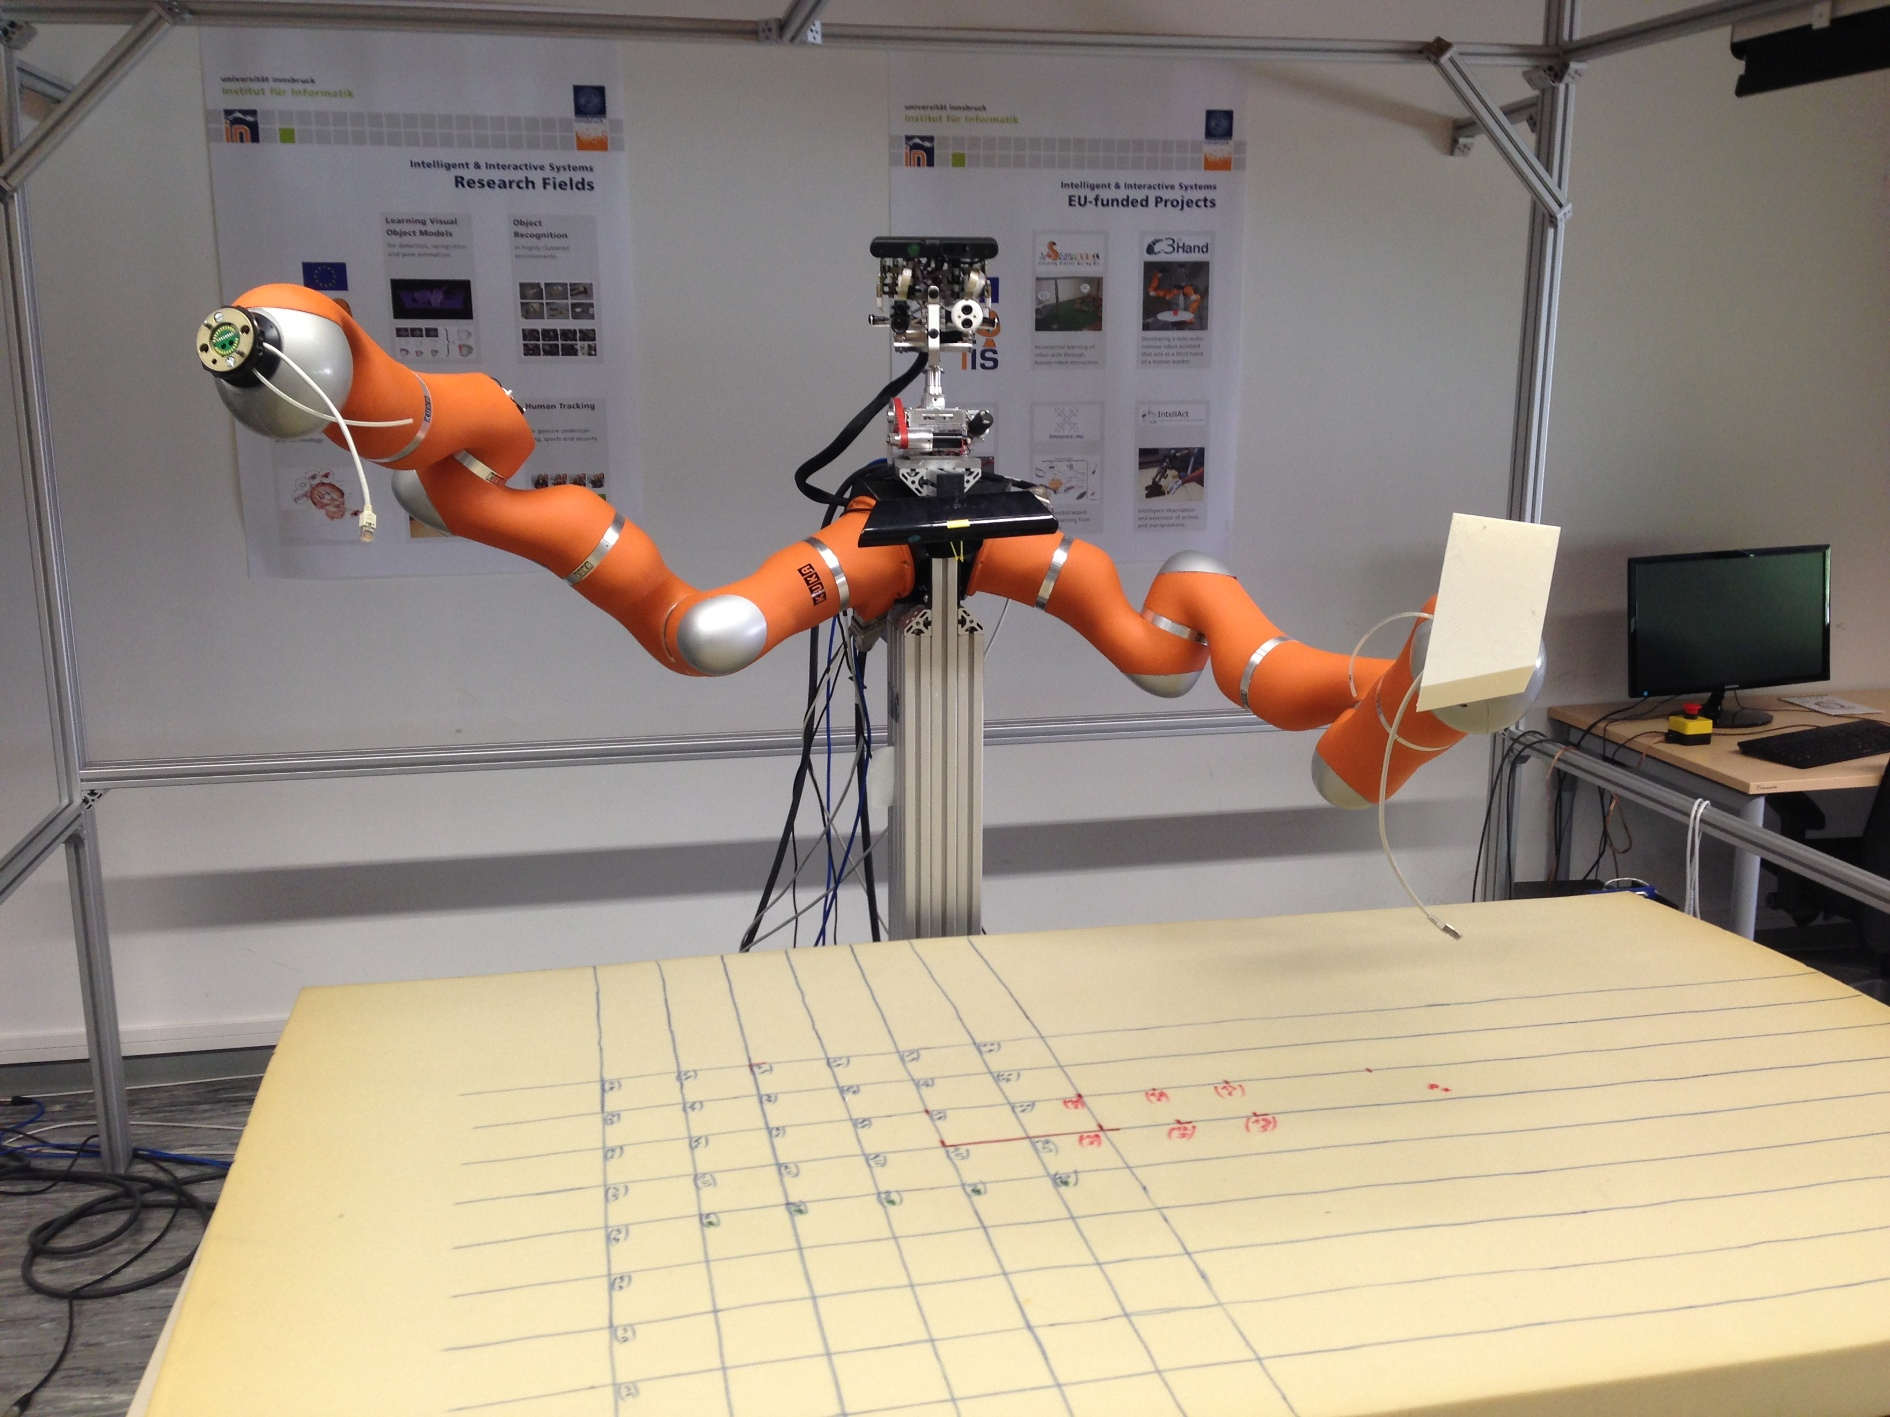
\includegraphics[width=0.75\textwidth]{images/robot_setup.jpg}
	\caption{Current setup in the IIS-Lab}
	\label{fig:iis_setup}
\end{figure}

The robot setting, that was considered in this thesis can be seen in Figure \ref{fig:iis_setup}
The main part of the robot setup in the IIS-Lab consists of an aluminium torso with two mounted KUKA light weight robot arms. Those arms have 7 degrees of freedom (DOF) each one can carry up to 7kg of payload. Additionally a Schunk SDH gripper can be mounted on each arm.

\begin{itemize}
	\item \textbf{KUKA LWR 4+ arm}\\
		Description of the arm(7 DOF, max. 7kg payload, 16kg weight, very flexible,...
	\item \textbf{Schunk SDH gripper}\\
		Description of the gripper(3-finger-gripper, different grasp types, as powerful as human hand, very sensitive)
	\item \textbf{Kinect camera}\\
		Description of Kinect(RGB camera, Depth sensor, 3d data under any light conditions)
\end{itemize}


\section{The Robot Operating System(ROS)}

The implementation of the project requirements is based on ROS. Therefore a brief introduction about the basic concepts\footnote{http://wiki.ros.org/ROS/Concepts} shall be given here. The explained terminology will be used throughout this thesis. As stated in \cite{quigley2009}, ROS is not an operating system in the classical sense. It runs on top of a host operating system (usually linux) and can be seen as an additional communication layer, providing various mechanisms for inter process communication. A ROS system consists of a number of \emph{nodes}. Each node is an independent computation unit that runs in it's own process, adding some clearly defined functionality to the overall system. For example one node can be responsible for planning, another one for perception and a third one for controlling the hardware. Nodes communicate to each other by passing \emph{messages}, using the ROS communication infrastructure. Messages are strictly typed data structures, defined in a special message composition format\footnote{http://wiki.ros.org/msg}. They can be composed of primitive types like float, integer or string, but also of other message types. Therefore it is possible to create arbitrary complex messages for each use case. Messages are published to \emph{topics}. A topic is a strongly typed message bus, addressed by it's \emph{topic name}. Arbitrary nodes can connect to a topic in parallel, as long as they use the correct message type. Each node can publish and subscribe to a number of topics. It is also possible that various nodes publish to the same topic. 

Topic names are strings, used to identify topics. They can be organized into \emph{namespaces} to build a tree hierarchy comparable to the directory structure in a file system. This is very important, as for example the simulator should use similar topic names as the real robot. The namespace concept allows both instances to use identical names but each one in it's own namespace. The following samples represent valid topic names:
\begin{itemize}
\item \texttt{/} (this is the root namespace)
\item \texttt{/topic}
\item \texttt{/component/topic}
\item \texttt{/namespace/component/topic}
\end{itemize}

The communication via ROS topics is asynchronous - involved nodes may even not be aware of each others existence. Synchronous message exchange between nodes happens via ROS \emph{services}. In contrast to topics, a service with a given name can only be offered by one single node. Services are addressed, using the same naming strategy as topics. The service message is composed of a request and a response part. A client node that sends a service request will block, until the advertising node has handled the request and delivers a response. The concept of ROS topics and services is shown in Figure \ref{fig:ros_concept}
\begin{figure}[h]
	\centering
  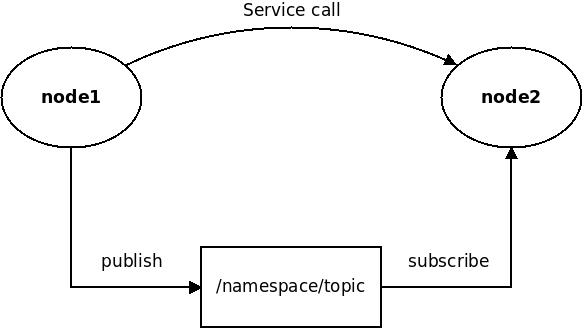
\includegraphics[width=0.5\textwidth]{images/ros_concept.jpg}
	\caption{ROS nodes, topics and services}
	\label{fig:ros_concept}
\end{figure}

The nodes of a ROS system can be distributed over various different machines. One of them has to be the dedicated \emph{ROS master}. The master is responsible to handle topic and service registrations and holds information about the involved ROS nodes. Other machines connect to the master via network. The ROS master also provides a centralized \emph{parameter server}. This is a shared dictionary that can be used to store and retrieve configuration data and other shared parameters. Nodes can access the parameter server at runtime and read or modify it's content. \\

A system usually consists of a large number of nodes that have to be configured and started. This can be done, using so called \emph{launch files}. Those are simple textfiles, holding startup information and configuration details for one or more nodes in an XML like syntax. Using the \emph{roslaunch} command line tool, a whole system of nodes can be configured and launched at once. \\

ROS is a modular software system organized into \emph{packages}. Each package adds clearly defined functionality and can be reused in other systems. Packages can be installed on demand and they may also depend on the functionality of other packages. A package might contain one or more ROS nodes or even only configuration data. Additional packages can be downloaded and installed, using a package manager tool.
Custom functionality is added to a ROS system by creating a new package and developing the required piece of software.

\section{Project Targets}
Both objectives

	\begin{itemize}
	
		\item \textbf{Simulation}\\
			Realistic replication of the robot setup on a suitable simulation platform
			Generation of realistic sensor data
			Visualization of collisions
			Implementation of a ROS interface, corresponding to that one of the real robot
		\item \textbf{Motion Planning}\\
			Configuration and integration of a motion planning framework
			Implementation of a benchmark pick and place task, executable on simulator and
			real robot
			Provide an easy to use interface to the planner
			Analyse the quality of the various planning algorithms
			
	\end{itemize}
% Simulation
%!TEX root = thesis.tex

\chapter{Robot simulation}
\label{chap:simulation}

This chapter focuses on the simulation part of the thesis. The objective is the creation of a simulation model, particularly designed for the IIS lab robot setup. This model needs to reflect the properties of the robot arms and the grippers as good as possible and provide physically similar behaviour. Certainly the simulated components have to provide the same control interface as their real counterparts, allowing to test and optimize control code on the simulator before utilizing it on the real robot. Preferably the control code does not differentiate between the two runtime environments. The requirements to such a solution can be summarized as follows: 

\begin{itemize}

\item
The simulator needs to be able to generate realistic sensor and feedback data that can be used by the control software. This includes forces and torques that are measured within joints and tactile sensors, the current state of the various robot joints (position, velocity, effort) and also RGB and depth images, that are usually produced by Kinect cameras.

\item
The simulation solution has to provide exactly the same ROS control interface as the real robot. This interface essentially consists of a number of ROS topics, that can be used to send control commands to the various different robot components or to read actual joint states and sensor data.
 
\item
The utilized simulation platform has to provide a graphical user interface that allows to visualize the motions of the robot and its interaction with the environment. Possibly accidental collisions of  robot parts have to be registered and should also be visualized.

\item
In order to be used by as many people as possible, it is very important that the solution is really easy to use and does not require a long training. Therefore we put particular focus on usability and documentation.

\end{itemize}

The following sections explain the realization of this simulation solution step by step. The introduction section gives an overview about dynamic simulations and the requirements for the utilized simulation platform. After that the chosen simulation platform V-Rep is introduced and general information about the concepts and used terminology is given. Subsequent sections focus on the necessary steps to achieve the final solution, namely modelling required robot components, assembling and configuring the simulation scene and the implementation of the ROS control interface.

\section{Introduction}

Realistic simulation requires models that exactly describe the physical properties of the involved objects. A robot is formed from rigid elements called \emph{links}, connected by \emph{joints}. A link is a three-dimensional body with a specific mass and moment of inertia. The texture of its surface depends on the utilized material. Joints are the flexible connections between the links. They are usually actuated by motors with a certain strength. Properties like the velocity of the robot's motions or the maximum possible payload it is able to bear depend on the strength of its motors. The sum of those physical parameters describes the dynamic properties of the robot. \\

The robot is used to perform motions and interact with objects within its environment. If the robot arm collides with an object it produces a collision reaction. The nature of this collision reaction depends on the physical parameters of the robot and the involved object. If the object is immovable, the robot motion will be stopped at a certain point. If the robot tries to grasp and lift a heavy object, it might slip through its fingers because the surface of the object may be to smooth and the gripper is not able to apply enough force to hold the object. \\

The required solution should be able to provide a realistic simulation of such dynamic interactions and reflect the physical behaviour of the robot as good as possible. Therefore the utilized simulation platform has to make use of a \emph{physics engine}. A physics engine is a software component, that is capable of computing parameters of physical processes based on the dynamic properties of the involved objects. Examples of such engines are the Open Dynamics Engine\footnote{http://www.ode.org} (ODE) and Bullet physics\footnote{http://bulletphysics.org}. We selected the simulation platform by taking the following criteria into account:

\begin{itemize}
\item
Which physics engine is used or is it possible to choose among various engines?
\item
Usability and stability
\item
Expandability
\item
Availability of required model components (arm model, gripper,\ldots)
\item
Quality of the documentation
\item
Licence issues
\end{itemize}

Candidates that have been taken into account were the Gazebo\footnote{http://gazebosim.org/} simulator and V-Rep\footnote{http://www.coppeliarobotics.com}. We finally decided to implement our project based on the V-Rep simulation platform because during initial tests it seemed to be much more stable than Gazebo and the user interface is very intuitive. Another important point was that V-Rep ships with a fully functional model of the Kuka LWR4+ robot arm.

\section{The Virtual Robot Experimentation Platform(V-Rep)}

This section gives an overview of the utilized simulation platform. V-Rep is a robot simulator, developed and maintained by Coppelia Robotics. The current version (V3.1.2) allows to choose among three configurable physics engines, namely ODE, Bullet and Vortex (only trial version) for simulating dynamic processes. The simulation environment is modelled, using the included scene editor. The distribution contains a large number of predefined models for different robot types. Additional modules provide functionalities related to collision visualization (\emph{collision detection module}) and inverse kinematics calculation (\emph{IK calculation module}). The behaviour of the simulator is highly customizable and its functionality can be extended via plugins. A plugin is a software library that is written in C++ and interacts with the simulator by using the provided programming API. V-Rep also allows to add embedded scripts to specific simulations. Those scripts need to be written in the scripting language LUA\footnote{http://www.lua.org}. V-Rep is no open source software but it provides a free licence for educational units and can therefore be used for research purposes. \cite{freese2013} gives a detailed insight into the V-Rep simulation platform.

%That editor can also be used to edit and simplify meshes. This is very important because for simulating dynamic processes only simple shapes with a low amount of vertices, edges and faces should be used to reduce complexity. The contained model browser provides a rich set of different robot models, static objects and various sensors, ready to use. A powerful feature are V-Rep's so called \emph{calculation modules}. They can be configured to provide additional calculation functionalities on groups of scene objects. The \emph{collision detection module} is capable of detecting and visualizing all kinds of collisions within the simulation scene. The \emph{inverse kinematics calculation module} allows to solve inverse kinematics problems for manipulators. The behaviour of the simulator is highly customizable via a rich programming API for C++ as well as the scripting language LUA\footnote{http://www.lua.org}. V-Rep is no open source software but it provides a free licence for educational units and can therefore be used for research purposes. \cite{freese2013} gives a more detailed insight into V-Rep's concepts .

\section{Dynamic simulations in V-REP}
\label{sec:vrep_intro}

For a better understanding of the modelling process it is necessary to explain a few fundamental concepts about designing simulations in V-Rep. This section covers the aspects that are important for the underlying project along with the used terminology. A detailed explanation can be found in the official V-Rep documentation\footnote{http://www.coppeliarobotics/helpFiles}. \\

Simulations in V-Rep are organized into \emph{scenes}. A scene represents the simulated world which is composed from a number of elements like three dimensional bodies, joints, sensors or cameras that are combined in a tree structure and arranged within the environment. This tree structure forms the \emph{scene hierarchy}. The elements within that hierarchy are called \emph{scene objects}. The scene hierarchy can be modified in the \emph{scene hierarchy view}, located on the left hand side of the scene editor. V-Rep provides various types of scene objects, but only those, which are important for the implementation will be explained here.

\begin{itemize}
\item \textbf{Shape} \\
Rigid objects like robot links or parts of the furniture are represented as shapes. V-Rep distinguishes between primitive shapes (cylinder, cuboid, sphere, plane and disk) and complex shapes (triangle meshes). Various shapes can be combined to groups and therefore treated as one single object. Shapes can be defined to be \emph{static} or \emph{non-static}. The position of a static object is fixed relative to its parent node within the scene hierarchy. Non-static objects underlie gravity and will fall down if they are not constrained by a joint or a rigid connection. It is also necessary to distinguish between \emph{respondable} and \emph{non-respondable} shapes. Respondable shapes are handled by the physics engine and create collision reactions when colliding with other respondable objects during simulation. Therefore their physical attributes like mass, moment of inertia and material settings need to be clearly defined. Non-responable shapes are visible in the scene but they do not create collision reactions. Shapes allow to set additional attributes that specify special properties, used by other modules of the simulator. The \emph{collidable} attribute states that the shape is considered by the collision detection module. The \emph{renderable} attribute marks a shape to be recognized by a vision sensor.

\item \textbf{Joint} \\
A joint is a flexible connection between two rigid parts of a robot. All the joints that were used within this project are \emph{revolute} joints which allow the rotation on a single-axis. Those joints are actuated by a motor. The motor settings include maximum force or torque and velocity limits. V-Rep supports joint control in three different modes:
\begin{itemize}

\item \textbf{Torque/force mode} \\
The behaviour of a joint in \emph{torque/force} mode is simulated by the physics engine, based on the specified motor limits. The joint is operated by a simulated controller that allows to set a target position. The controller then actuates the joint towards the commanded target position. This is the most realistic control mode as the dynamic parameters of the joint motor and the connected bodies are taken into account.

\item \textbf{Inverse kinematics mode} \\
A joint in \emph{inverse kinematics mode} is controlled by V-Rep's IK calculation module. The configuration option \emph{hybrid operation} specifies, that the dynamic parameters of the joint are also taken into account.

\item \textbf{Dependent mode} \\
Operating a joint in \emph{dependent mode} means that its position depends on the position of another joint within the scene. This dependency is formulated as \emph{dependency equation} which calculates a target position based on the current position of the connected joint.

\end{itemize}
The configuration of the angular joint limits is defined based on a minimum position and the maximum possible opening angle. 

\item \textbf{Vision sensor} \\
A vision sensor is a simulated image capturing device. Each vision sensor captures images depending on its location within the scene and the configured opening angle and resolution. It is able to produce sequences of RGB and depth images.

\item \textbf{Force sensor} \\
A force sensor in V-Rep is used to rigidly connect two non-static, respondable shapes. The force sensor then measures the linear forces and and angular torques that act upon this connection. It is also possible to define a maximum force the connection is able to bear. When this maximum value is exceeded, the connection will break.

\item \textbf{Dummy} \\
Dummies are the simplest scene objects but they provide important functionality for the various modules of V-Rep. Dummies are used to explicitly define the origin of a specific reference frame, e.g. the world reference frame or the base of a robot arm. Other scene objects can then be configured to be child objects of such dummies within the scene hierarchy. Their relative placement can then be adjusted with respect to that reference frame. Two dummies can also be linked as \emph{tip-target pairs} to be used by the IK calculation module. This functionality is explained in section \ref{sec:config_ik}.

\end{itemize}

Groups of scene objects can be organized in \emph{collections} and treated as one single entity. Collections play an important role in the collision detection module. Let $\mathcal{A}$ and $\mathcal{B}$ be two distinctive collections of collidable shapes. The collision detection module allows to explicitly check collection $\mathcal{A}$ for collisions against collection $\mathcal{B}$. Collections also allow to override the collidable or renderable settings of all contained shapes. The configuration of the collision detection module is explained in section \ref{sec:config_col}. \\

Scene objects can be loosely arranged within the scene hierarchy or be part of a \emph{model}. A model is a subtree of elements within this hierarchy that logically belong together, as they form a specific object like a robot arm or a table. The root element of this model tree is called the \emph{model base}. Models can be saved in model files and therefore be reused in various different scenes. Robot models are composed from rigid bodies called \emph{links}, connected by joints that allow to actuate the flexible parts of the simulated robot component. Each link is usually represented by two different shapes. The first one forms the visual geometry and is usually a non-respondable, complex shape. The second shape forms the collision geometry which has to be a simplified approximation of the visual geometry, composed from groups of primitive shapes. That shape states the respondable part of the robot link as it is seen by the physics engine and needs therefore appropriate configuration of the dynamic parameters. That part is usually invisible but very important as it applies realistic behaviour to the model and allows it to interact with other respondable objects within the scene. Without respondable parts, the model would just move through other bodies as only respondable shapes are able to produce collision reactions. \\

This separation into visual and respondable parts is necessary because V-Rep and the utilized physics engines are not able to use arbitrarily complex shapes for dynamics calculations. Utilized meshes have to fulfil at least the \emph{convex} criteria\footnote{A line between any two vertices of the mesh lies completely within the mesh boundaries}, but the V-Rep documentation recommends to use groups of primitive shapes for the collision geometry to increase the simulation performance. The V-Rep scene editor provides a special \emph{shape edit mode} that allows to edit and simplify meshes and to extract different types of primitive shapes from a selection of vertices. The shape edit mode can be entered by selecting the desired shape and then click the item \texttt{Tools -> shape edition} from the menu bar or the corresponding tool bar button.

\begin{figure}[ht]
	\centering
  	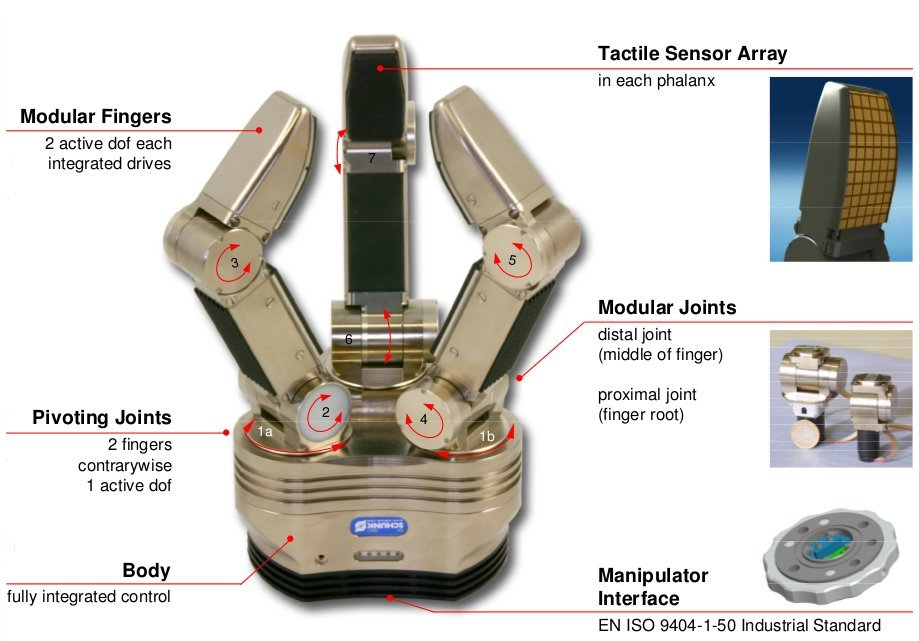
\includegraphics[width=1.0\textwidth]{images/sdh_sheet.jpg}
	\caption{Schunk SDH-2 gripper}
	{\scriptsize Image source: \cite{schunk2010}}
	\label{fig:sdh_sheet}
\end{figure}

\section{Designing the simulation scene}

This section explains in detail the structure of the simulation scene and the contained models. The setup contains three types of robot components - the Kuka LWR4+ robot arm, the Schunk SDH-2 gripper and the Kinect camera. For each one of them, a simulation model was required in order to be able to build up the scene. V-Rep ships with a realistic and fully functional model for the Kuka arm and the Kinect camera. But as there was no model for the Schunk SDH-2 robot hand available, we had to create it from scratch. The necessary steps of this modelling process are explained in the next section.

\subsection{Modelling the Schunk SDH-2 gripper}

Figure \ref{fig:sdh_sheet} shows the Schunk SDH-2 hand. The gripper has 3 fingers, each one containing two modular joints. The joints located closer to the wrist are called the \emph{proximal} finger joints whereas the joints, actuating the finger tips are called the \emph{distal} finger joints. The joints 1a and 1b in figure \ref{fig:sdh_sheet} can be rotated along their vertical axis though their rotation angles are codependent. That means if one finger rotates to the left, the other one is rotated to the right by the same angle, actually adding one additional degree of freedom. Those two joints are called the \emph{pivoting} joints. \\

\begin{figure}[t]
	\centering
  	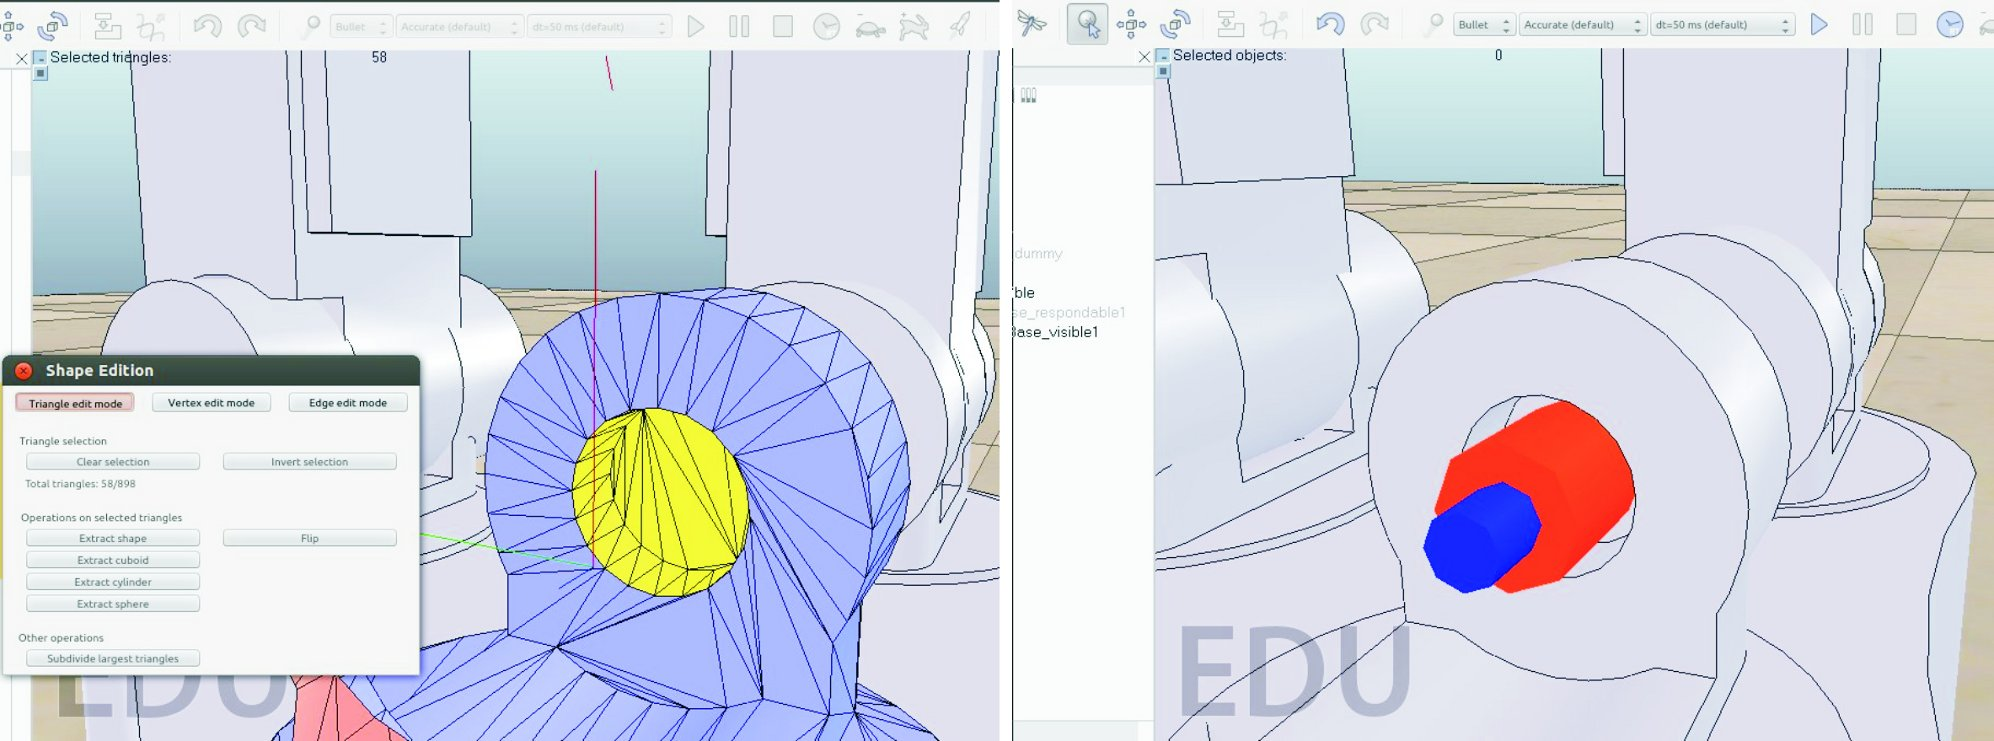
\includegraphics[width=1.0\textwidth]{images/place_joint.jpg}
	\caption{Placing a joint within the model}
	\label{fig:place_jnt}
\end{figure}

The visual part of the hand model basically consists of 4 different shapes - the gripper body, finger knuckles, finger links and finger tips. Suitable meshes were taken from the \path{schunk_description}\footnote{http://wiki.ros.org/schunk\_description} ROS package and imported into the V-Rep editor. They have then been arranged according to the technical description in \citep{schunk2010}. The next step was to connect those parts by the corresponding joints. \\

The correct placement of those joints is very important to achieve the desired transformations of the actuated parts when changing the joint angles. Therefore it was necessary to determine the correct position and orientation for each single joint within the model. Each flexible part of the gripper has cylinder shaped holes at the locations where the parts are connected by joints. Those holes also exist in the utilized meshes and they were used to extract the correct joint placement locations. This was achieved by selecting the vertices within the mesh that form the area, where a specific joint had to fit. From that selection a cylinder was extracted, using the corresponding editor functionality. The origin of that cylinder's reference frame which is located in the cylinder center stated the exact place location for the corresponding joint. After creating a new joint on that location, the extracted cylinder could be removed again. Those steps had to be repeated for all 8 gripper joints. This placement process is visualized in figure \ref{fig:place_jnt}. The left image shows the extraction of the target area. On the right image, the joint is already placed on its appropriate location.
\begin{figure}[h]
	\centering
  	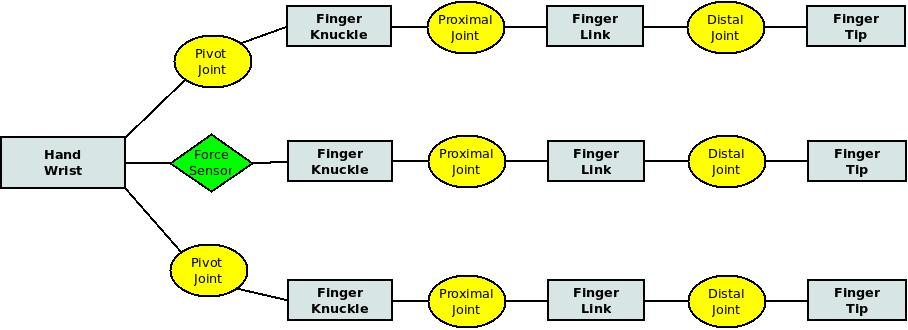
\includegraphics[width=1.0\textwidth]{images/hand_tree.jpg}
	\caption{Kinematic chain of the Schunk gripper}
	\label{fig:hand_tree}
\end{figure}\\

After placing all the joints and links within the scene, the model tree was adjusted to form the kinematic chain of the hand as can be seen in figure \ref{fig:hand_tree}. The dynamic parameters of the joints were set according to the technical description in \citep{schunk2010}. The configured values are listed in table \ref{tbl:tech_data}. As the positions of the pivoting joints are connected to each other, the configuration of the second finger's pivoting joint had to be set sightly different. To achieve this mirroring behaviour the joint is operated in the dependent mode and its dependency equation $f$ is defined as $f(x) = -x$ where $x$ is the position of the first finger's pivoting joint.
\begin{table}[h]
  \centering
  \begin{tabular}[h]{|l|c|c|c|c|} \hline
	\textbf{Joint type} & \textbf{pos. min.} & \textbf{pos. max.} & \textbf{max. effort} & \textbf{max. velocity} \\ \hline
	Pivoting joints & $0^{\circ}$ & $90^{\circ}$ & $5.0 Nm$ & $210^{\circ}/s$ \\
	Proximal joints & $-90^{\circ}$ & $90^{\circ}$ & $2.1 Nm$ & $210^{\circ}/s$ \\
	Distal joints & $-90^{\circ}$ & $90^{\circ}$ & $1.4 Nm$ & $210^{\circ}/s$ \\ \hline
  \end{tabular}
  \caption{Joint dynamic parameters}
  \label{tbl:tech_data}
\end{table} \\

The visual part of the gripper model was formed by the utilized meshes. The next step in the design process was to define the collision geometry that was used to model the underlying physics. We decided to do that by approximating the original shape by groups of primitive shapes. This was achieved by executing the following steps for each part of the model:
\begin{itemize}
\item
The shape edit mode was used to locate and select parts of the mesh that could be approximated by either a cuboid or a cylinder. The extraction was done by selecting groups of suitable vertices with the mouse while holding the \texttt{shift} button.
\item
Those parts were then extracted as primitive shape by using the corresponding editor functionality.
The extraction process is visualized in figure \ref{fig:ex_pure_shape}.
\item
Those steps had to be repeated until the most important parts of the shape were extracted that way. After that all extracted shapes were grouped into one single shape.
\item
The respondable flag was activated for the resulting shape and the dynamic parameters were adjusted accordingly. The mass values and the inertial matrix have been provided by Alex Rietzler who had already evaluated those values for his own project. The material settings were left at the default value which is the predefined \emph{highFrictionMaterial}. This material has a friction coefficient of 1.0 which is the maximum possible value but it uses no linear or angular damping.
\item
For the name of the extracted shape the same value was used as for its visual counterpart but the \path{_respondable} suffix was appended. The suffix allows to easily identify the respondable model parts within the scene hierarchy. 

\item
The extracted shapes were then removed from the active visibility layer because they are just used for dynamics calculations.
\end{itemize}

\begin{figure}
	\centering
  	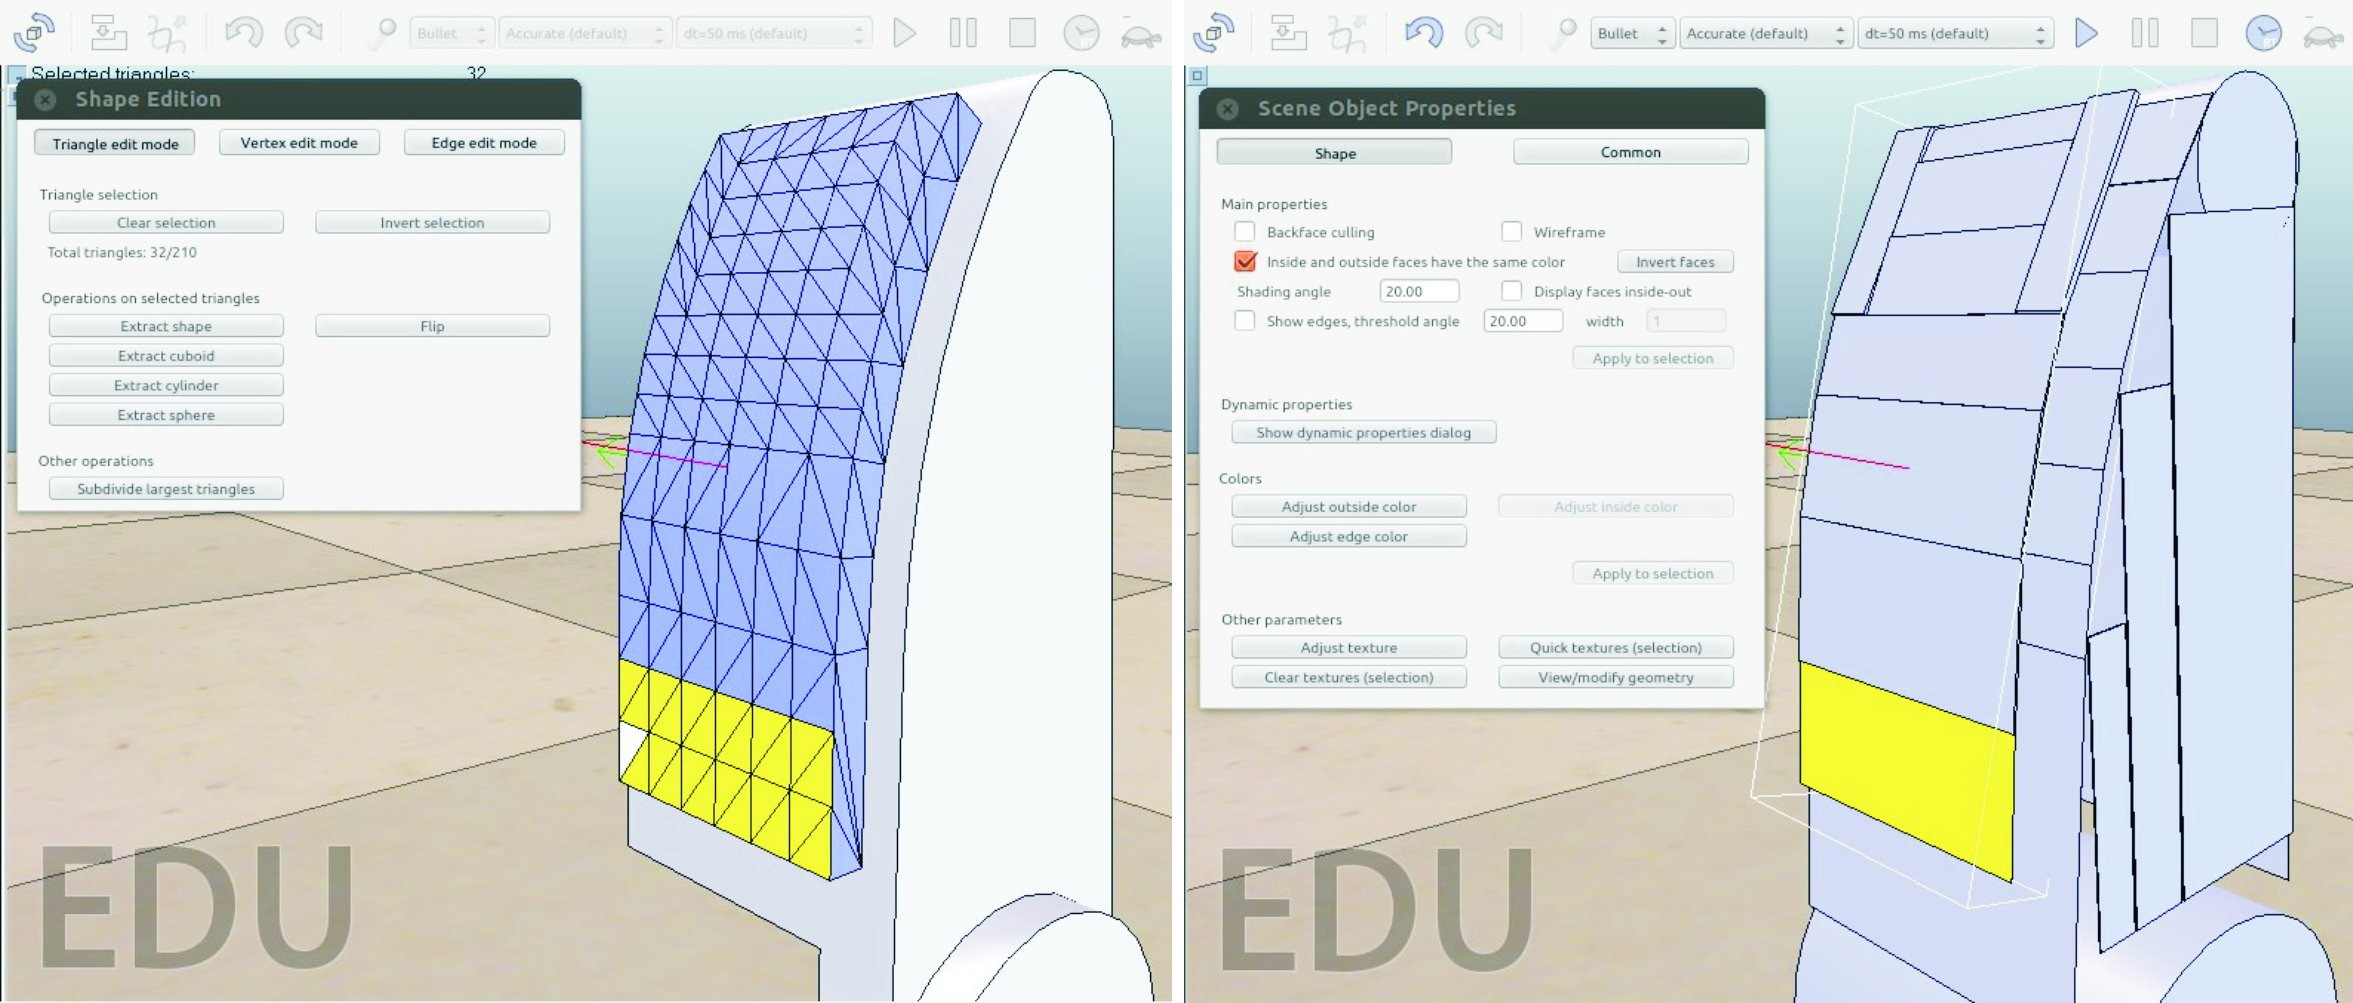
\includegraphics[width=1.0\textwidth]{images/extract_pure_shapes.jpg}
	\caption{Process of approximating the original mesh with pure shapes}
	\label{fig:ex_pure_shape}
\end{figure}

The last step of the modelling process was the adjustment of the model tree. This adjustment was done by rearranging the nodes within the scene hierarchy view. Root element of the hand model is the respondable part of the gripper body which was also defined to be the dedicated model base. At this point it is very important to follow the V-Rep guidelines for designing dynamic simulations because if the hierarchy is wrong, the model will simply fall apart when starting the simulation (detailed information about that topic can be found in the corresponding chapter\footnote{http://www.coppeliarobotics.com/helpFiles/en/designingDynamicSimulations.htm} of the V-Rep dodumentation). Each non-static and respondable shape needs to be connected to its parent by a joint or a force sensor. The visual part of the link is always a child object of its corresponding respondable. That way, the kinematic chain of the gripper was formed. The resulting model tree is shown in figure \ref{fig:gripper_tree}.
\begin{figure}[ht]
	\centering
  	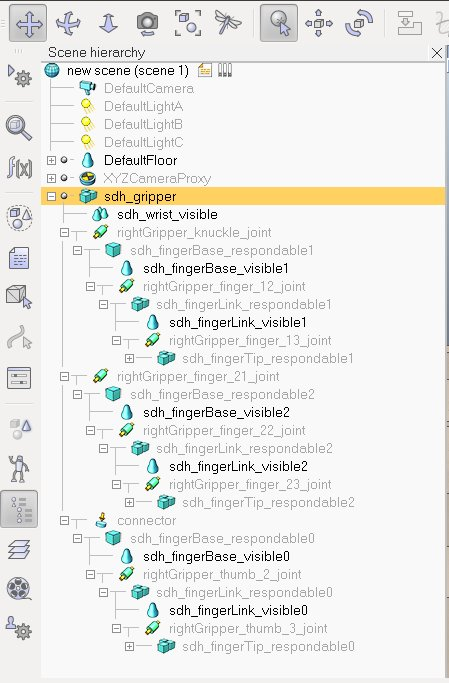
\includegraphics[width=0.4\textwidth]{images/gripper_tree.jpg}
	\caption{Gripper model tree}
	\label{fig:gripper_tree}
\end{figure}

\subsection{Assembling the scene}

\begin{figure}[hbt]
	\centering
  	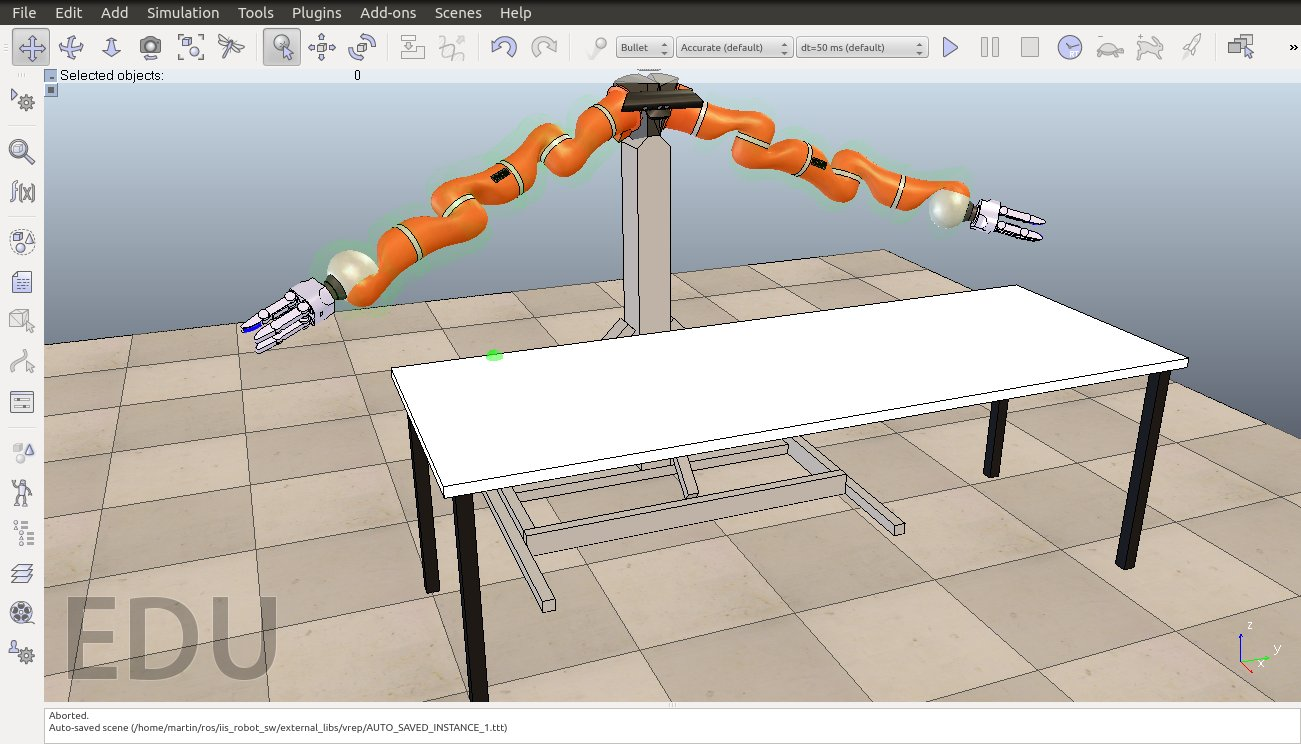
\includegraphics[width=0.8\textwidth]{images/simulation_scene.jpg}
	\caption{Structure of the V-Rep simulation scene}
	\label{fig:sim_scene}
\end{figure}

After finishing the gripper modelling process, each necessary component was available to build up the simulation scene as can be seen in figure \ref{fig:sim_scene}. The final scene consists of a model of the robot's torso, two Kuka LWR4+ arm models with attached grippers and a model of the table in front of the robot. The origin of the world reference frame is located on the upper left side of the table, indicated by a slightly green shimmering sphere. A dummy object called \path{ref_frame_origin} was placed at that location. Each position for the simulation is defined relative to this dummy element. If it is necessary to change the origin of the world reference frame, this can simply be achieved by just adjusting the position and orientation that dummy. The positions and orientations of the torso, the table and the two arms were set relative to the world reference frame. The grippers were placed on the tip of each arm. Within the scene hierarchy they are child elements of the last node in the corresponding arm tree. The correct rotation and offset was measured on the real counterpart and then adjusted accordingly. \\

The plate and the legs of the table were modelled as group of primitive cuboids. The table shape is respondable to ensure that it will produce a collision reaction if a robot component collides with it. But as it is a static object its position will not be influenced by such a collision because it is fixed within the scene. The material setting is set to the default \emph{highFrictionMaterial}. \\

The utilized Kinect camera model was contained in the V-Rep distribution and just had to be inserted into the scene. Position and orientation of the Kinect camera with respect to the robot base was measured in the real world and adjusted accordingly in the simulator. Figure \ref{fig:sim_scene_tree} shows a part of the resulting scene tree for the final simulation scene. 

\begin{figure}[h]
	\centering
  	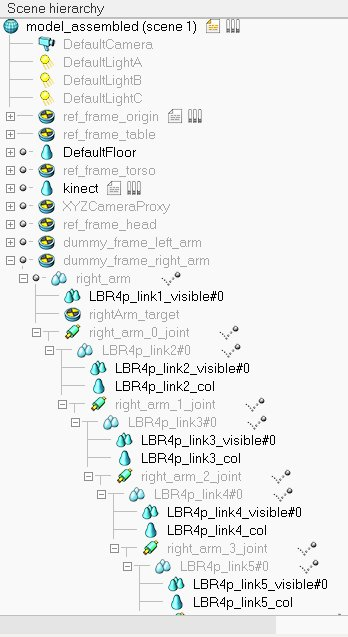
\includegraphics[width=0.4\textwidth]{images/scene_tree.jpg}
	\caption{Simulation scene hierarchy}
	\label{fig:sim_scene_tree}
\end{figure}

\subsection{Configuring the collision detection module}
\label{sec:config_col}

The final solution needs to be able to detect and visualize collisions of the simulated robot with itself or its environment. This section describes the utilized simulator functionality along with the necessary steps to achieve the desired behaviour. \\

V-Rep's \emph{collision detection module}\footnote{http://www.coppeliarobotics.com/helpFiles/en/collisionDetection.htm} is capable of detecting and visualizing collisions between (collections of) shapes. The shapes used for this collision detection can be any shapes within the scene as long as they are defined to be \emph{collidable}. It is important to note that the collision detection module only \textit{detects} collisions by checking for interferences between meshes. Handling \emph{collision reactions} is the responsibility of the  physics engine. Configuration of the collision detection module is done by registering one or more \emph{collision objects}. Each collision object consists of a \emph{collider} and a \emph{collidee}. The collider can be for example the robot arm and the collidee a collection of objects, the arm is not allowed to collide with. Both of them can be single shapes or collections of shapes. The big advantage in using collections is that they allow to exactly describe which shapes should be checked against which other ones. It is also possible to configure a collection to overwrite the collidable attributes of the contained shapes. That means a whole collection can be marked to be collidable even though the contained shapes are not. The collidee settings also offer the option \emph{all other collidable objects in the scene}. In that case, the collider is checked against all collidable shapes in the scene that are not part of the collider itself. Detected collisions are visualized by applying different colouring either to the collider or to the collidee. Each collision object needs to be \emph{handled}, which means the collision detection module has to be triggered to check for collisions and visualize them as defined for the specific collision object. This can happen automatically in each simulation step or it can be triggered manually by using the corresponding API function. The desired behaviour is defined by a configuration option called \emph{Explicit handling} in the collision object properties. \\

\begin{figure}[h]
	\centering
  	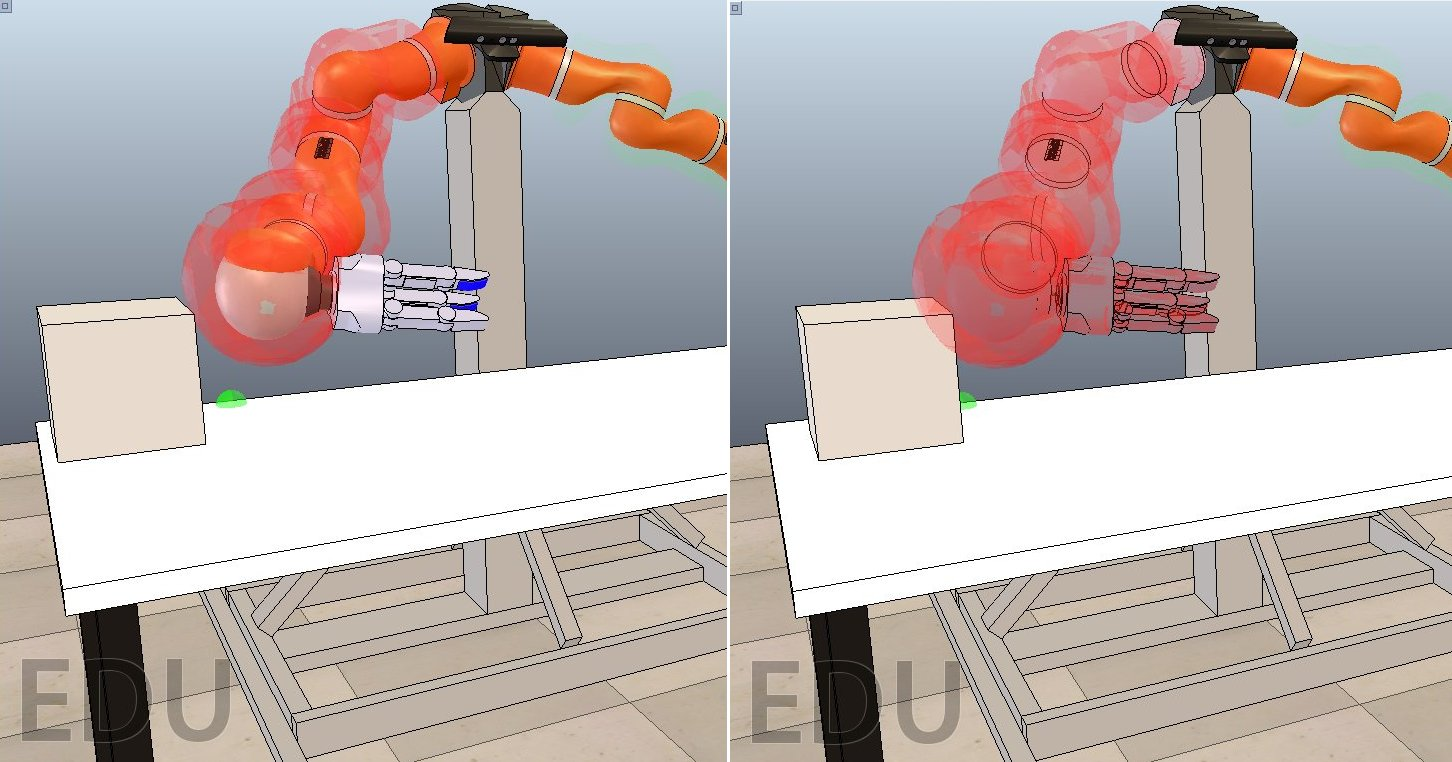
\includegraphics[width=0.8\textwidth]{images/collision.jpg}
	\caption{Collision detection and visualization}
	\label{fig:collision}
\end{figure}

One of the aims of the solution is to allow to check actions in the simulator before executing them on the real robot. Therefore the simulator needs to be able to detect and visualize collisions that possibly happen during those actions. Moreover it would be a convenient feature to have a proximity warning if parts of the robot come dangerously close to an obstacle during movement. To achieve that goal, we decided to create an enlarged version of the robot arm geometry which we called the \emph{collision shield} and do additional collision checking. These considerations lead to the two different types of possible collisions which we called \emph{soft collisions} and \emph{hard collisions}. Soft collisions are collisions, detected on the collision shield of the model. They just indicate a warning that the robot comes very close to an object it is not allowed to touch. \emph{Hard collisions} describe a direct hit of a robot part on another object. This would be also a collision in the real world. The final solution is able to distinguish between those two types as can be seen in figure \ref{fig:collision}. The left image shows a soft collision, the right image indicates a hard collision.\\

The first step during realization was to model the collision shield. Therefore it was necessary to create an additional shape for each single link of the robot arm that is slightly larger than the original one. The images in figure \ref{fig:shield_steps} show snapshots of this modelling process. For all links within the arm models the following steps had to be performed:

\begin{itemize}
\item
Create a copy of the shape that forms the visible part of the robot link
\item
Morph the copied object into a group of convex shapes to reduce complexity. This can be done by using the corresponding shape editor functionality (figure \ref{fig:shield_steps}a).
\item
Ungroup the resulting group of shapes and merge them into one single shape (figure \ref{fig:shield_steps}b).
\item
Grow the bounding box of the resulting shape, but only in x and y direction. The resulting mesh should be 10cm larger but keep the same height (figure \ref{fig:shield_steps}c).
\item
Adjust the outside color to make it green and nearly transparent. The collision shield should be visible but not occlude the original model (figure \ref{fig:shield_steps}d).
\item
Apply a meaningful name to the newly created shape to be be able to easily identify it within the model hierarchy. Here the name of the original shape with the \path{_col} suffix was used.
\item
Place the new shape as child element of the corresponding respondable shape within the model tree to ensure that the shield element correctly moves when actuating the arm model.
\item
Adjust the shape object properties. Define the new shape to be \emph{static} and \emph{non-respondable} because it is not intended to produce any collision reactions.
\item
Disable the \emph{collidable} flag on the shape. This behaviour will be overridden in the collection
settings later on when configuring the collision detection module.
\end{itemize}

\begin{figure}[h]
	\centering
  	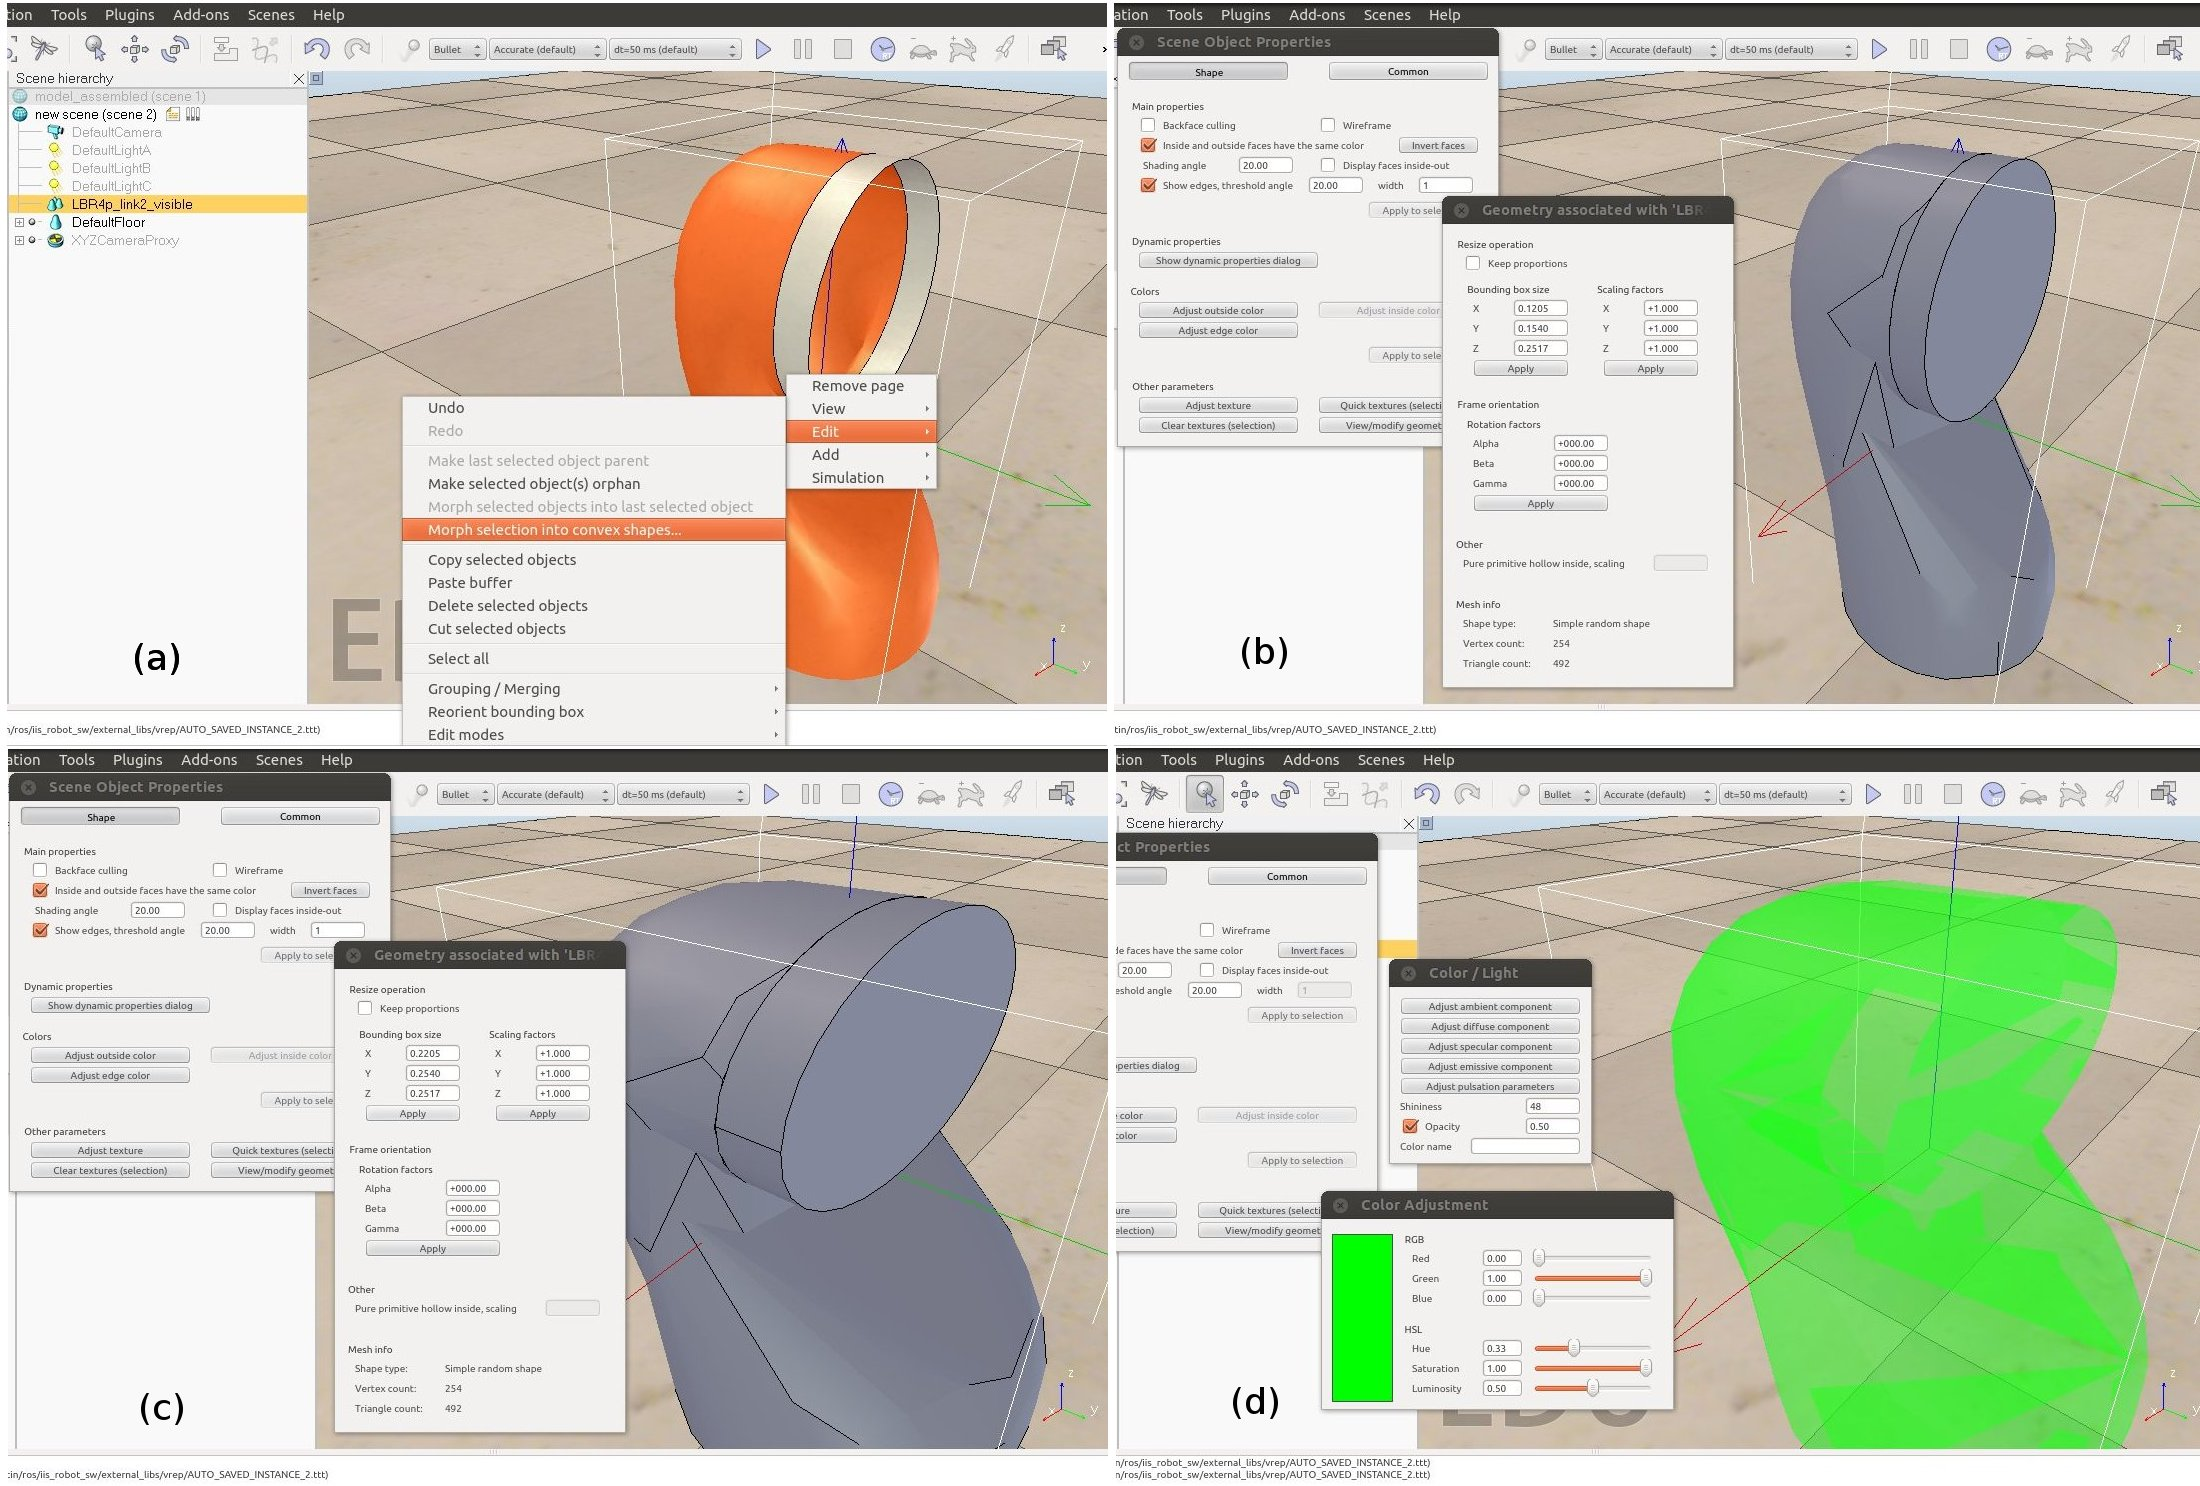
\includegraphics[width=1.0\textwidth]{images/shield_steps.jpg}
	\caption{Modelling steps for the second arm link}
	\label{fig:shield_steps}
\end{figure}

\begin{table}
  \centering
  \begin{tabular}[h]{|l|l|l|} \hline
	\textbf{Collision object} & \textbf{Collider} & \textbf{Collidee} \\ \hline
	left\_arm & leftArm & all other entities \\
	right\_arm & rightArm & all other entities \\
	left\_armShield & leftArmShield & exLeftArmShield \\
	right\_armShield & rightArmShield & exRightArmShield \\ \hline
  \end{tabular}
  \caption{Configured collision objects}
  \label{fig:col_groups}
\end{table}

\begin{table}
  \centering
  \begin{tabular}[h]{|l|l|} \hline
	\textbf{Collection} & \textbf{Definition} \\ \hline
	leftArm & $\{~s~|~s\in\textit{subtree of left arm}~\}$ \\
	leftArmShield & $\{~t~|~t\in\textit{element of left collision shield}~\}$ \\
	exLeftArmShield & $\{~u~|~u\in\textit{scene and}~u~\notin\textit{subtree of left arm}~\}$ \\
	rightArm & $\{~v~|~v\in\textit{subtree of left arm}~\}$ \\
	rightArmShield & $\{~w~|~w\in\textit{element of left collision shield}~\}$ \\
	exRightArmShield & $\{~x~|~x\in\textit{scene and}~x~\notin\textit{subtree of right arm}~\}$ \\ \hline
  \end{tabular}
  \caption{Collection definitions}
  \label{fig:col_defs}
\end{table}

The next step was to define the required collision objects in the configuration of the collision detection module. The collision objects were created as listed in table \ref{fig:col_groups}. The collection definitions that were used for the collider and collidee settings can be seen in table \ref{fig:col_defs}.
Each arm requires two collision objects - one for hard collisions and another one for soft collisions. The responsibility of the collision objects named \path{left_arm} and \path{right_arm} is to check for hard collisions. The colliders (collections named \path{leftArm} and \path{rightArm}) are checked for collisions against \emph{all other collidable objects in the scene}. This setting is only possible because the collidable flag is disabled within the scene object settings of the collision shield elements as mentioned above. That means that they are excluded from collision checking by default. The collision objects, named \path{left_armShield} and \path{right_armShield} are responsible to check for soft collisions. The colliders (collections \path{leftArmShield} and \path{rightArmShield}) contain only the collision shield elements of the corresponding arm models. As those elements were defined without the \emph{collidable} flag, the option \emph{Collection overrides collidable properties} was selected in the collection settings to explicitly enforce collision checking when using those collections. The collections, defining the collidees (\path{exLeftArmShield} and \path{exRightArmShield}) include all other objects in the scene \emph{except} those, contained in the left/right arm's subtree. This exclusion is necessary because otherwise those collision objects would also detect collisions between the shield elements and the other arm links.\\

All collision objects are defined not to be handled explicitly. It is necessary to first check for direct hits before looking for shield hits because a direct hit always implies a shield hit. Therefore the collision objects have to be handled sequentially and for soft collisions is only checked if no hard collision was detected before. Handling those collision objects happens from code and will be explained later on in the section about control interface implementation.

\subsection{Configuring the IK calculation module}
\label{sec:config_ik}

The ROS control interface requires the robot arm to be controllable in joint space and in Cartesian space, depending on the selected control mode. Joint space targets are relatively easy to handle as that only means to set the target position of each single arm joint. Setting targets in Cartesian space requires to solve the \emph{inverse kinematics} (IK) problem which is defined by \citep{craig2005} as the problem of finding a possible joint configuration for the robot to achieve a desired end effector position and orientation. This section describes the IK functionality provided by the V-Rep simulator along with necessary configuration steps.\\

The \emph{inverse kinematics calculation module}\footnote{http://www.coppeliarobotics.com/helpFiles/en/inverseKinematicsModule.htm} allows to define and register \emph{IK groups}. An IK group is capable of solving IK problems for a simulated manipulator like our robot arm. It consists of one or more so called \emph{IK elements} and configuration settings for the utilized IK calculation method. IK elements are used to define the kinematic chain, constraints and desired precision settings. The kinematic chain is specified by configuring the dedicated \emph{base} link and the \emph{tip}. The tip is a dummy object, indicating the end effector reference frame. It needs to be linked to a \emph{target} dummy, forming a \emph{IK, tip-target} connection which is done by selecting the appropriate link type within the dummy object settings. The IK goal pose is set by placing that target dummy at the desired location. IK elements can be configured to enforce position constraints and/or orientation constraints for each single axis. The precision settings define the maximum allowed deviation (linear and angular) between desired and achieved end effector position to consider a solution to be correct. \\

\begin{figure}[htb]
	\centering
  	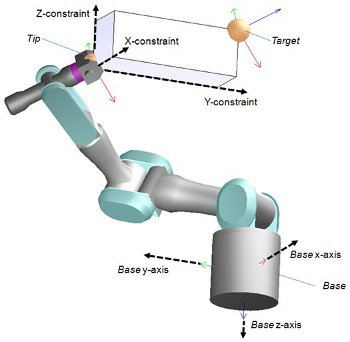
\includegraphics[width=0.5\textwidth]{images/ik_vrep.jpg}
	\caption{IK calculation module concept}
	{\scriptsize Image source: http://www.coppeliarobotics.com/helpFiles/en/solvingIkAndFk.htm}
	\label{fig:ik_vrep}
\end{figure}

The IK calculation module allows to define various IK groups for each robot component with differing configurations. Along with the IK elements, the IK group settings include the desired calculation method and the maximum amount of calculation iterations to use. Available IK calculation methods are \emph{pseudo inverse} (PI) and \emph{damped least squares} (DLS). As stated by \cite{buss2004}, the PI method is usually faster than DLS. The tradeoff is that PI tends to be unstable in configurations where the target position is unreachable. That fact leads to a jittery behaviour of the manipulator. The DLS method provides higher stability in such situations but requires more calculation time and is therefore slower. \\

A target pose in Cartesian space is set by adjusting the position and orientation of the IK target dummy. Then it is necessary to \emph{handle} one more of the responsible IK groups which follows the same approach that is used for the collision objects described above. The IK calculation module tries to adjust the joint configurations of the corresponding manipulator until the tip pose matches the target pose, respecting joint limits and configured constraints. Figure \ref{fig:ik_vrep} shows a schematic description of that concept. The joints within the kinematic chain need to be operated in \emph{inverse kinematics mode}, otherwise they can not be controlled by the IK calculation module. This can be specified within the joint settings. \\

\begin{table}[h]
  \centering
  \begin{tabular}[h]{|l|c|c|c|} \hline
	\textbf{IK group} & \textbf{Method} & \textbf{Iterations} & \textbf{Prec. lin/ang} \\ \hline
	left\_arm & PI & 9 & 0.001 / 0.1  \\
	left\_arm1 & PI & 3 & 0.002 / 0.2  \\
	left\_arm2 & DLS & 3 & 0.002 / 0.1  \\
	right\_arm & PI & 9 & 0.001 / 0.1  \\
	right\_arm1 & PI & 3 & 0.002 / 0.2  \\
	right\_arm2 & DLS & 3 & 0.002 / 0.1  \\ \hline
  \end{tabular}
  \caption{IK group definitions}
  \label{fig:ik_defs}
\end{table}

Three IK groups have been created for each arm contained in our simulation scene. The configuration settings are listed in figure \ref{fig:ik_defs}. They were chosen, following the guidelines in the V-Rep documentation. The precision settings specify the tolerance values that have to be enforced by the corresponding IK group. The first two groups use the faster PI calculation method. The first one allows a higher amount of maximum iterations while demanding stricter precision settings than the second one. The third one is designed to increase stability especially for positions close to singularities. Therefore the DLS method was chosen with an increased position tolerance value. That configuration is slower because of the DSL calculation method and therefore it is only used if the other groups failed to find a solution. The IK groups are handled sequentially until one of them is able to solve the problem. This process is explained in the ROS control interface section later on.

\section{Implementing the ROS control interface}

\begin{figure}[htb]
	\centering
  	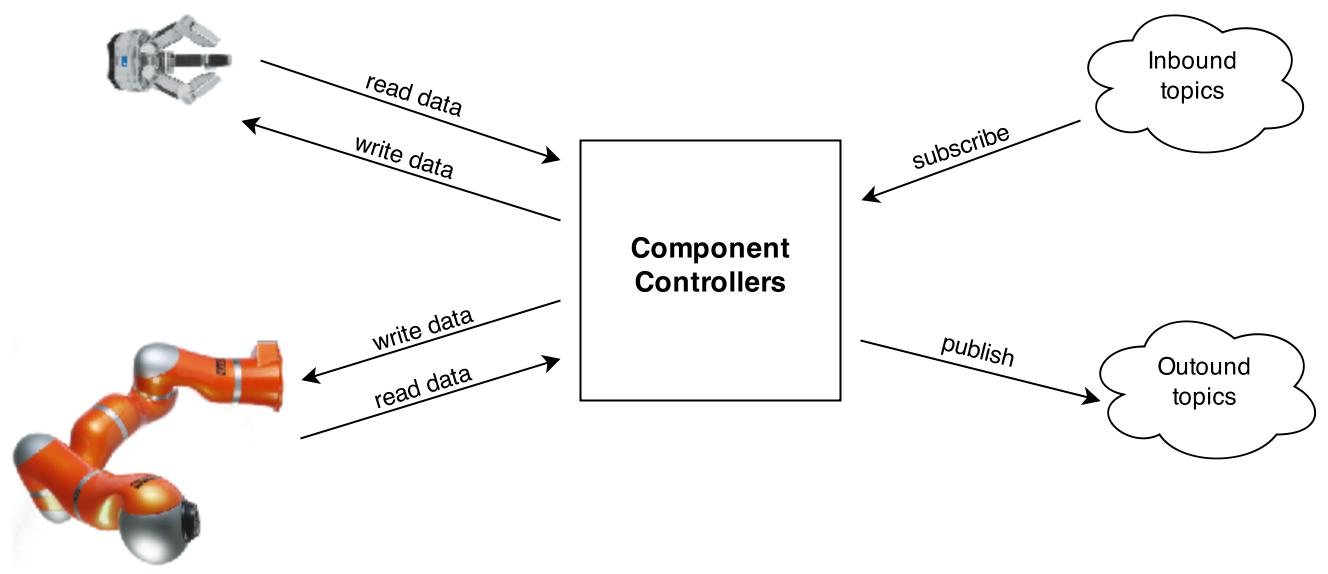
\includegraphics[width=0.8\textwidth]{images/control_flow.jpg}
	\caption{Control flow structure}
	\label{fig:control_flow}
\end{figure}

In the real world, the Schunk hand and the Kuka arm have their own, clearly defined ROS control interfaces. Those interfaces are composed from sets of inbound and outbound ROS topics that allow to send commands and to retrieve state data. The ROS topics are usually provided by a controller that writes commanded values to the hardware and reads the current state. The structure of this control flow is visualized in figure \ref{fig:control_flow}. The simulation models need to provide exactly the same ROS interface as their real counterparts, using the same topic names and message types. The existing ROS interface that is part of the V-Rep distribution is not suitable as it only provides a very general approach for controlling joint values and reading state data so it was necessary to create a custom solution that provides proper interfaces for the arm and hand models. \\

The V-Rep simulator provides various extension points, allowing to add custom functionality. We implemented the final solution as a simulator plugin, written in C++ and using V-Rep's \emph{regular API}\footnote{http://www.coppeliarobotics.com/helpFiles/en/apiOverview.htm}. A plugin is a software library that gets automatically loaded on V-Rep startup and interacts with the simulator via the provided API functions. The plugin architecture is described in section \ref{sec:plugin_arch}. As the robot setup in the IIS-Lab is frequently extended we put particular focus on the extendability of the plugin design. During project implementation, the IIS group acquired a new robot head that is also controllable via ROS. The provided solution can easily be extended to be able to handle simulation models for such new robot components. \\

One problem that arose during the implementation process was, how to identify simulation models that should be controlled by the plugin. V-Rep is a simulation environment that allows to load and simulate different environments and therefore the plugin functionality should not be tied to one specific scene. The current simulation scene contains the models of two Kuka arms and two Schunk grippers but the intended solution should be customizable. Maybe there should be another scene that only contains one arm model and no grippers at all. This requires the plugin to be able to detect known models in arbitrary simulation scenes and then provide the proper control interfaces. Section \ref{sec:comp_id} explains in detail how this problem was solved along with the utilized V-Rep functionality. \\

\subsection{Plugin architecture}
\label{sec:plugin_arch}

This section describes the architecture of the implemented simulator plugin along with the most important parts of the software. The source code can be found in the \path{iis_simulation} package that is part of the \path{iis_robot_sw} repository.\\

A plugin is a compiled library file that needs to be placed in the V-Rep working directory and follow the V-Rep specific naming conventions. On startup, V-Rep looks for library files, prefixed with \path{libv_repExt}. Matching files are automatically loaded. A plugin runs in the main simulation thread - that means it has to be programmed really carefully to avoid performance leaks during simulation. The plugin code is organized as can be seen in the UML diagram in figure \ref{fig:plugin_uml}. The major parts of the system are described in the subsequent paragraphs.

\begin{figure}
	\centering
  	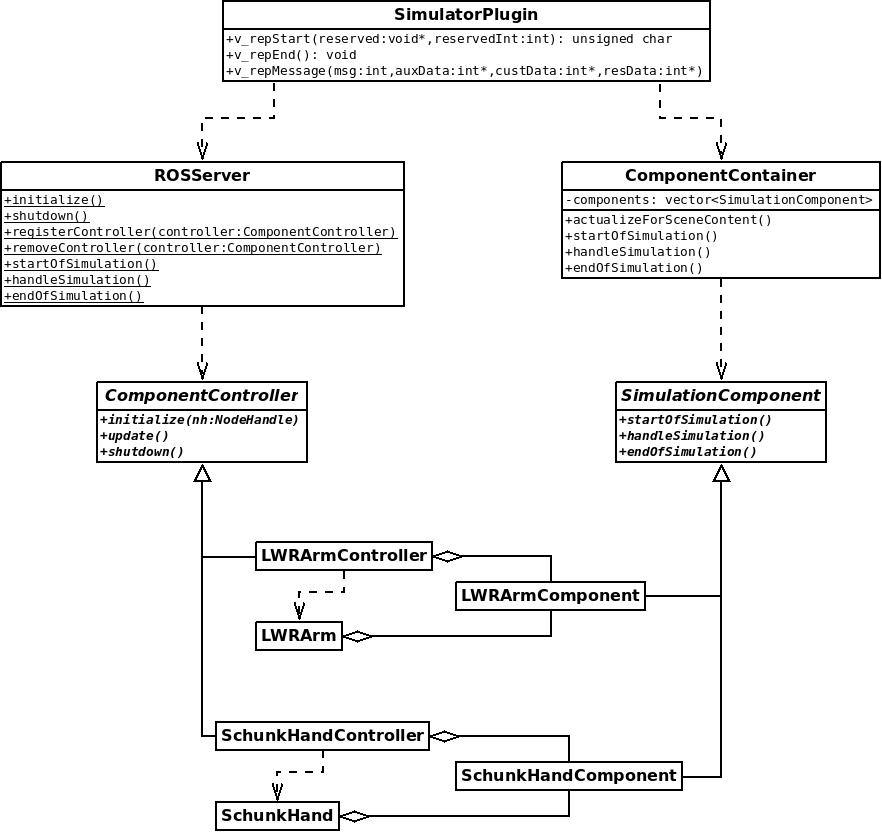
\includegraphics[width=0.8\textwidth]{images/SimulatorPluginUML.jpg}
	\caption{Simulator plugin architecture}
	\label{fig:plugin_uml}
\end{figure}

\paragraph{SimulationComponent}

We us the term \emph{simulation component} to describe a simulation model for a specific robot component that has to be handled by the plugin. Each simulation component provides its own clearly defined control interface. A simulation scene can contain multiple simulation components from various types. The \path{SimulationComponent} class is the abstract base class for all those simulation components. Currently there are existing two concrete implementations -- the \path{LWRArmComponent} and the \path{SchunkHandComponent}. If the scenario should be extended and new components have to be introduced, it is necessary to create a new subclass of \path{SimulationComponent} and provide implementations for the abstract methods. The methods \path{startOfSimulation()} and \path{endOfSimulation()} are called when a simulation is started/ended. The method \path{handleSimulation()} is invoked on each simulation step and can be used for example to handle IK groups or registered collision objects.

\paragraph{ComponentContainer}

This class represents the set of all identified simulation components within the current scene. On V-Rep startup an instance of \path{ComponentContainer} is created. When the plugin recognizes that the content of the current simulation scene has changed, the method \path{actualizeForSceneContent} of the \path{ComponentContainer} gets triggered. This method then performs the following steps:
\begin{itemize}

\item
It validates all currently registered \path{SimulationComponent} instances if they are still valid and present in the scene.
\item
It traverses the whole scene hierarchy to identify newly created components
\item
If a new component is identified, a corresponding concrete instance of \path{SimulationComponent} is created and added to the container.

\end{itemize}
  
During a running simulation, the \path{ComponentContainer} gets notified about each single simulation step. It then simply propagates that event to all registered \path{SimulationComponent} instances by invoking their \path{handleSimulation} methods. Those can then perform all necessary steps like triggering collision checking or handling IK groups.

\paragraph{ComponentController}

This is the abstract base class for all controllers. A controller actually represents the ROS interface of a specific simulation component, maintaining all the inbound and outbound topics used to control the simulated hardware. It is responsible for delegating commanded values to the underlying component as well as reading and publishing state data. Concrete implementations are the \path{LWRArmController} and the \path{SchunkHandController}. A \path{ComponentController} needs to be registered at the \path{ROSServer} and gets initialized on simulation start. Concrete implementations can use the provided \path{NodeHandle} to create all the necessary publishers and subscribers. The \path{update} method is called by the \path{ROSServer} on each simulation step and forces the controller to publish all the required data. The \path{shutdown} method is called by the \path{ROSServer} on simulation end, forcing the controller to shutdown all publishers and subscribers.
  
\paragraph{ROSServer}

The \path{ROSServer} is a static class that encapsulates all ROS related functionality. It tries to initialize ROS on plugin startup, forcing a shutdown, if the connection to the master cannot be established. Otherwise it creates and maintains a ROS \path{NodeHandle} for the \path{simulation} namespace. Each \path{SimulationComponent} can register \path{ComponentController} instances at the \path{ROSServer}. On simulation start it initializes all registered controllers with the maintained \path{NodeHandle}. The \path{ROSServer} gets also notified about each simulation step and forces the controllers to handle the received commands and publish all the necessary data. On simulation end it triggers the shutdown of all registered controllers.

\paragraph{SimulatorPlugin}

The \path{SimulatorPlugin} states the connection between the simulator and the other parts of the software. V-Rep communicates with a plugin, using a clearly defined interface that consists of 3 function definitions:

\begin{itemize}

\item \texttt{unsigned char v\_repStart(void* reserved,int reservedInt)} \\
This function is called on V-Rep startup and is used to perform necessary initialization steps. A return value of zero indicates that the initialization process failed and the plugin gets unloaded immediately.
Our implementation calls the \path{initialize()} method of the \path{ROSServer} class. If that initialization fails, the plugin is not able to work.

\item \texttt{void v\_repEnd()} \\
This function is called before V-Rep shutdown. Our solution performs necessary cleanup steps and frees all allocated memory.

\item \texttt{void* v\_repMessage(int msg, int* auxData, void* custData, int* resData)} \\
This function is called very often during the whole V-Rep lifecycle and is therefore very performance critical. Via this function the plugin gets notified about simulator events like start/end of simulation, simulation step, scene content change, scene switch and more. The event type is specified by the provided \path{msg} parameter. Our \path{SimulatorPlugin} then just passes those events to the software components that are responsible to handle the specific action by invoking the corresponding methods. For example simulation related events like start/end of simulation and simulation step are propagated to the \path{ROSServer} and the \path{ComponentContainer}. Table \ref{tbl:sim_msg} lists the messages that are handled by our implementation.

\begin{table}[ht]
  \centering
  \begin{tabular}{|l|l|} \hline
	\textbf{Message} & \textbf{Description} \\ \hline
	\path{sim_message_eventcallback_instancepass} & Indicates a scene content change \\
	\path{sim_message_eventcallback_moduleopen} & The simulation is about to start \\
	\path{sim_message_eventcallback_modulehandle} & Indicates a simulation step \\
	\path{sim_message_eventcallback_moduleclose} & End of simulation  \\ \hline
  \end{tabular}
  \caption{Simulator messages}
  \label{tbl:sim_msg}
\end{table}

\end{itemize}

Each simulation step is handled by the \path{SimulatorPlugin} as shown in figure \ref{fig:handle_sim}. The plugin receives the \path{sim_message_eventcallback_modulehandle} message from the simulator. It first asks the \path{ComponentContainer} to handle the simulation step which propagates that event to all registered \path{SimulationComponent} instances. After that, the \path{SimulatorPlugin} invokes the \path{handleSimulation} method of the \path{ROSServer}. The server then handles ROS related callbacks and forces the registered controllers to publish their state data.

\begin{figure}[ht]
	\centering
  	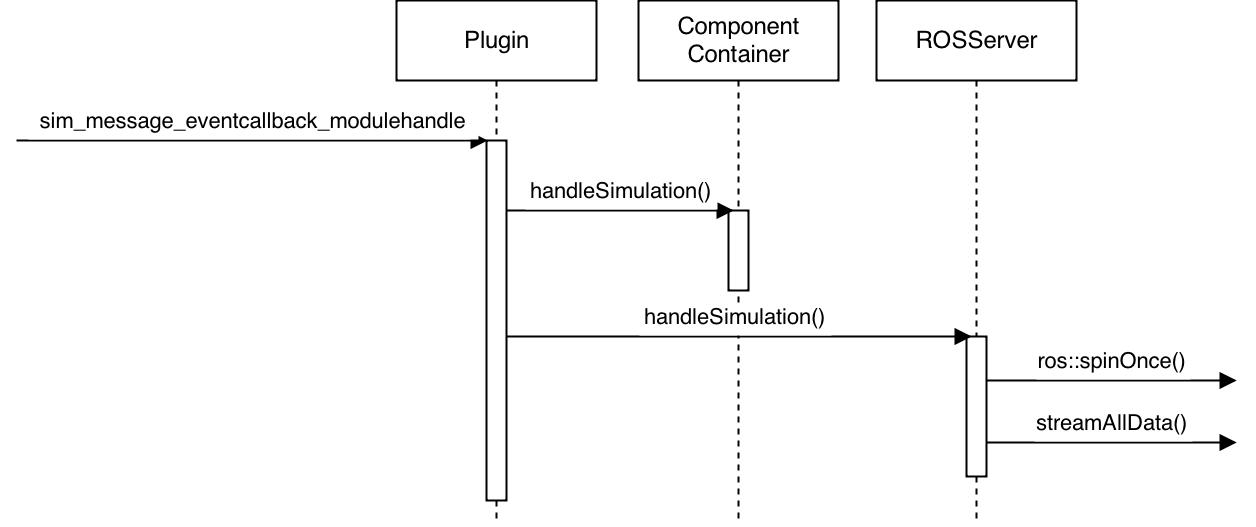
\includegraphics[width=1.0\textwidth]{images/handle_sim.jpg}
	\caption{Handling a simulation step}
	\label{fig:handle_sim}
\end{figure}

\subsection{Identifying simulation components}
\label{sec:comp_id}

\begin{figure}[h]
	\centering
  	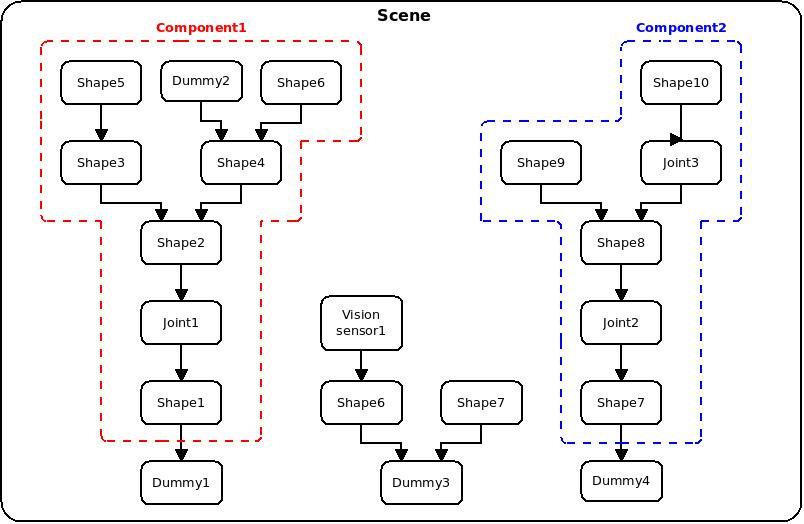
\includegraphics[width=0.8\textwidth]{images/scene_hierarchy.jpg}
	\caption{Sample scene hierarchy}
	\label{fig:scene_tree}
\end{figure}

The plugin functionality should not be tied to a specific simulation scene but to specific ``known'' models of robot components. For example adding a Kuka arm model to an arbitrary scene should force the plugin to create a corresponding controller that provides the proper ROS control topics. As visualized in figure \ref{fig:scene_tree}, each simulation scene is a hierarchy of different types of scene objects like joints, shapes, dummies or sensors. Those elements can be loose objects like a shape that was just added to the scene for a grasping simulation, but they could also be part of a simulation component like the Kuka arm or the Schunk gripper. Therefore the plugin needs to be able to identify subtrees of scene objects within this hierarchy that belong to such known models. Moreover, once a specific simulation component is identified, the plugin has to discover each part of the model tree as V-Rep does not provide a function that allows to determine all scene objects that belong to a specific model. Depending on the simulation component this can be the joints, force sensors or reference frame dummies. The scene objects in V-Rep are represented by their dedicated \emph{object handles}, which are simple integer values that uniquely identify specific objects within a scene. Interacting with scene objects using the V-Rep API requires those object handles to be known. For example setting the target position for a specific joint in the arm model requires to know the object handle that is associated to that joint. The goal of the identification process is to find the object handles of all scene objects that belong to the model. \\

\begin{figure}[h]
	\centering
  	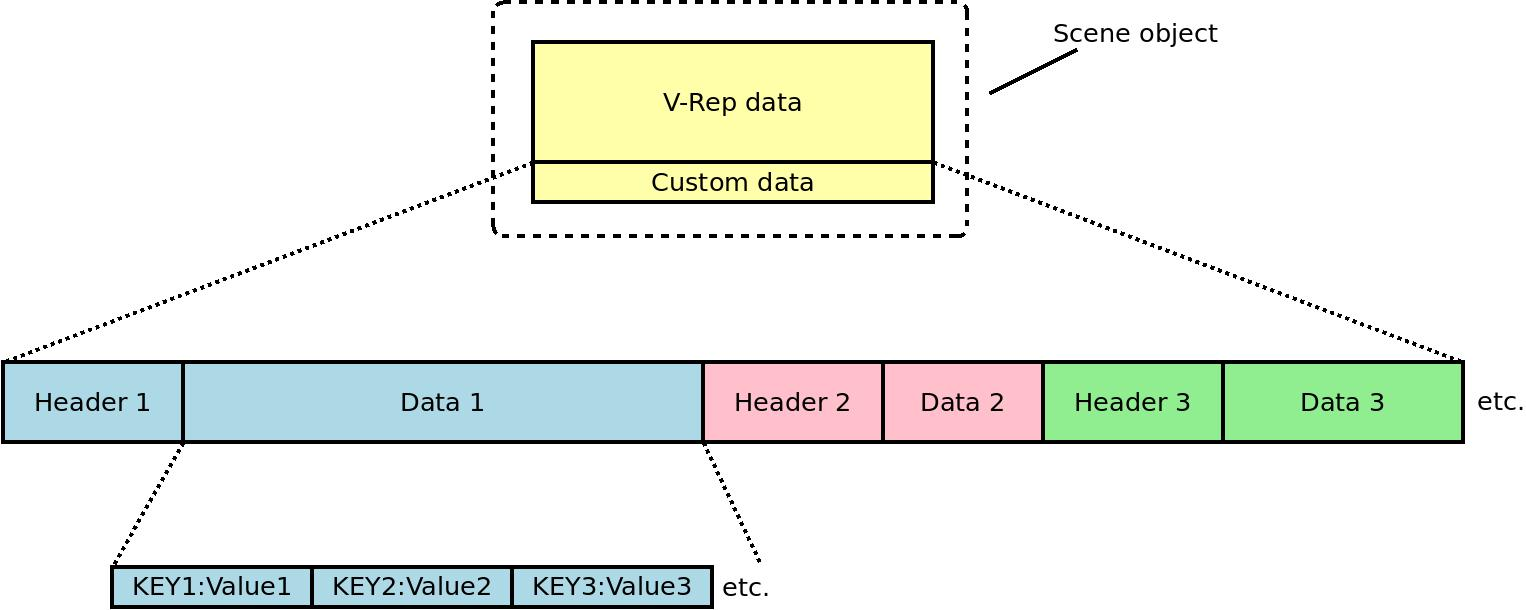
\includegraphics[width=0.8\textwidth]{images/custom_dev_data.jpg}
	\caption{Custom developer data segments on scene object}
	{\scriptsize Image source: http://www.coppeliarobotics.com/helpFiles/en/pluginTutorial.htm}
	\label{fig:cust_dev_data}
\end{figure}

We solved this identification problem by using so called \emph{custom developer data tags}. V-Rep allows to put auxiliary data segments to each single object in the scene. The data tags are configured in the scene object properties of the corresponding scene objects. This process is described in the documentation section in appendix \ref{app:sim_doc}. Each data segment starts with a header number which is used to uniquely identify the tag data from a specific developer. We used the number `2497' for the data segments used in this project. A visualization of this concept can be seen in figure \ref{fig:cust_dev_data}. The format of those data segments can freely be chosen by the developer. We decided to use string representations of key/value pairs, separated by a colon (:). The key is an integer value that specifies the type of information the tag contains. The value segment can be used to provide additional information, e.g. the name of the arm. The left arm's model base for example is tagged with the data segment 
\begin{center}
\texttt{2497,1:left\_arm}
\end{center}
The number 2497 is the header that identifies the data segment to belong to this plugin. The data segment identifies that scene object to be the model base of a Kuka arm model $(Key=1)$ with the name \path{left_arm}. Other tags are used to identify joints, force sensors and dummies that belong the the arm or gripper models. The available keys are explained in the sections that correspond to the specific simulation components. We have placed such developer data tags on all scene objects that are relevant to the plugin. \\

The plugin code was designed to react for scene content change. This happens when objects are added or removed from the current scene or when another scene gets loaded. When actualizing for scene content change, the \texttt{ComponentContainer} traverses the scene hierarchy and looks for objects, that are tagged as known components. On success, it creates the specific instance and adds it to the container. During initialization, the concrete \texttt{SimulationComponent} implementation then traverses the rest of the model subtree to extract all the remaining parts that belong to that specific model (joints, dummies, force sensors\ldots), also by looking for tagged objects. The implementations for arm and hand model provide feedback output on the console window about the status of this initialization process and provide meaningful error messages in case that not all necessary parts of a model could be successfully located.


\subsection{The LWRArmComponent}

The \path{LWRArmComponent} is a concrete subclass of \path{SimulationComponent} and states the abstraction of a simulated Kuka LWR4+ arm model. It is composed of two parts - an instance of the \path{LWRArm} class that provides access to the whole functionality of the arm model and a corresponding \path{LWRArmController} that is responsible for the ROS interface. The \path{LWRArmComponent} registers its controller at the \path{ROSServer} on simulation start. Both classes are explained in the following paragraphs.

\paragraph{LWRArm}

This class states the abstraction of the simulated hardware of the arm, providing methods to set commanded values and access all available state data. On creation, it is passed the object handle of the model base element as constructor argument. The base is identified by the \path{LWR_ARM_COMPONENT} tag. The value segment of this tag states the name of the arm which has to be unique within the scene. During initialization it traverses the model tree and extracts all required parts by searching for tagged scene objects as described in the previous section. The parts to identify are the 7 arm joints, the force sensor on the last link of the arm, IK tip and target dummies. The corresponding tags are listed in table \ref{fig:lwr_tags}. \\

\begin{table}[ht]
  \centering
  \begin{tabularx}{\textwidth}{|l|l|l|X|} \hline
	\textbf{Constant} & \textbf{Key} & \textbf{Value} & \textbf{Description} \\ \hline
	LWR\_ARM\_COMPONENT & 1 & Arm name & Identifies Kuka LWR arm model \\
	LWR\_ARM\_JOINT & 12 & Joint name & Joint in Kuka LWR arm \\
	LWR\_ARM\_CONNECTOR & 13 & - & Force sensor on arm tip \\
	LWR\_ARM\_TIP & 14 & - & IK tip dummy \\
	LWR\_ARM\_TARGET & 15 & - & IK target dummy  \\ \hline
  \end{tabularx}
  \caption{Tag data items for LWRArmComponent}
  \label{fig:lwr_tags}
\end{table}

To fulfil the requirements for the ROS control interface, the arm needs to be able to operate either in joint control mode (FK mode) or in inverse kinematics mode (IK mode). During FK mode the joints are operated in \emph{torque/force} mode and accept target positions to be set. Therefore the \path{LWRArm} class provides a method called \path{setJointTargetPositions}. This method expects a vector, containing the desired joint target positions and delegates the commanded values to the corresponding arm joints. \\

During IK mode the joints have to be operated in \emph{inverse kinematics} mode, which means that they are controlled by V-Rep's IK calculation module. Therefore we implemented the method \path{setKinematicsMode} in the \path{LWRArm} class that uses the appropriate V-Rep API function (\path{simSetJointMode}) to switch all joints to the required mode. Setting a target pose in Cartesian space is done by placing the IK target dummy at the required location and orientation. This can be done by using the method \path{setTargetPose} of the \path{LWRArm} class. When the arm is operated in IK mode, the method \path{handleIK} is invoked on each simulation step. This method uses the API function \path{simHandleIKGroup} to handle the previously configured IK groups sequentially, until one of them is able to solve the problem and set the proper joint target positions. If all of the fail, the arm will be at least in a configuration that states an approximate solution to the problem. \\

The IK group object handles are determined during initialization based on their names (API function \path{simGetIkGroupHandle}). One IK group which uses the same name as the arm model is mandatory, leading to a configuration error message if no such group can be found. Subsequent groups are optional and must have the same name with consecutive numbering. For example an \path{LWRArm} class with name \path{right_arm} searches for IK groups named \path{right_arm1}, \path{right_arm2}\ldots. We chose that naming strategy because it allows to reconfigure the IK calculation module and introduce additional IK groups without touching the plugin code. \\

The \path{LWRArm} class also provides a method that returns the current collision state of the underlying arm model. Therefore it requires the handles of the configured collision objects which are also searched during initialization based on the arm name (API function \path{simGetCollisionHandle}). The collision objects, responsible for soft collisions and hard collisions are required. An \path{LWRArm} class with name \path{right_arm} for example searches for collision objects named \path{right_arm} and \path{right_armShield}. If one or both of them cannot be detected, an error message is stated on the console and the collision detection functionality will not work as expected. The collision objects are handled by the \path{LWRArm} class on each simulation step (API function \path{simHandleCollision}). The collision object that is responsible for detecting direct collisions is handled first. If that one detects a collision, a direct hit is reported and it is not necessary to handle the second object at all, because a direct hit always implies a shield hit as well. Only if no direct hit was detected, the second collision object is handled. The outcome can be queried, using the method \path{getCollisionState} of the \path{LWRArm} class. The possible return values are listed in table \ref{tbl:col_states}. \\

\begin{table}[h]
  \centering
  \begin{tabular}{|c|l|} \hline
	\textbf{State} & \textbf{Description} \\ \hline
	0 & no collision at all \\
	1 & hard collision \\
	2 & soft collision \\ \hline
  \end{tabular}
  \caption{Possible collision states}
  \label{tbl:col_states}
\end{table}

\paragraph{LWRArmController}

The \path{LWRArmController} is a subclass of \path{ComponentController} that encapsulates the whole ROS interface for the \path{LWRArmComponnt}. On creation it is passed a reference to the underlying \path{LWRArm}. The controller listens on different ROS topics that allow to set target positions in joint space or Cartesian space, depending on the current \emph{control mode}. We implemented 4 basic control modes - \emph{joint control}, \emph{Cartesian control}, \emph{stop} and \emph{follow} mode. Joint control, follow and stop mode require the underlying \path{LWRArm} to be operated in FK mode. For Cartesian control mode, the arm needs to be switched to IK mode. The available control modes are explained as follows:

\begin{itemize}

\item \textbf{Joint control mode} \\
The \path{LWRArmController} accepts target positions in joint space via the \path{joint_control/move} topic and the underlying \path{LWRArm} is operated in FK mode. The message basically consists of a vector, containing the desired target angles for for all arm joints, measured in \emph{radiant}. Target positions received by the controller are validated to not exceed a specified \emph{velocity limit}. The aim of this velocity limit is to prevent the arm from doing rapid motions. This is achieved by enforcing the constraint
\begin{equation}
  |c_{i}-t_{i}|<\delta, \forall ~i~\in~[0,6]
\end{equation}
where $c_{i}$ are current and $t_{i}$ are received target positions for the joints 0 to 6 and $\delta$ is the current velocity limit. If the velocity limit is violated, the message is dropped and a corresponding error message is published to the \path{sensoring/error} topic and written to the console output. The default limit is set to a value of 0.1 and can be adjusted via the \path{joint_control/set_velocity_limit} topic. Valid target positions are simply passed to the \path{setJointTargetPositions} method of the underlying \path{LWRArm} instance.

\item \textbf{Cartesian control mode} \\
The controller accepts target positions in Cartesian space via the \path{cartesian_control/move} topic. Therefore, the \path{LWRArm} needs to be operated in IK mode. There is also a Cartesian velocity limit enforced for the received target pose. The constraint is defined as
\begin{equation}
  |c_{x}-t_{x}|<\sigma ~and~ |c_{y}-t_{y}|<\sigma ~and~ |c_{z}-t_{z}|<\sigma
\end{equation}
where $c$ is the current and $t$ is the received target position in Cartesian space and $\sigma$ is the current Cartesian velocity limit. The velocity limit can be adjusted, using the \path{cartesian_control/set_velocity_limit} topic. Invalid messages are dropped and result in an error message as well, published in \path{sensoring/error} topic. Valid target poses are passed to the underlying \path{LWRArm}, by using the method \path{setTargetPose}.

\item \textbf{Stop mode} \\
The arm does not accept any movement commands at all. Ongoing motions will be stopped immediately when switching the arm into this control mode. This is done by switching the underlying \path{LWRArm} to FK mode and then setting the target positions of all joints to their current position.

\item \textbf{Follow mode} \\
We designed the follow mode to mirror the behaviour to the real robot arms. Therefore this mode is only in the  simulation solution available. The controller reads the joint states of its real counterpart from the corresponding ROS topic and uses its current position as target. Therefore, the \path{LWRArm} is operated in FK mode. This results in an exact copy of the real robot's motions. We used this mode to test the accuracy of the simulation model by carefully moving the robot arm close to positions where it collides with the table and check when collisions were detected in the simulation. 

\end{itemize}

This section only covered the implemented control modes and the corresponding ROS topics but the controller also offers a number of topics that allow to retrieve state data like current joint positions, Cartesian position, the collision state and more. A complete interface description, containing all available ROS topics and the corresponding message types can be found in the documentation, located in appendix \ref{app:sim_doc}.

\subsection{The SchunkHandComponent}

The design of the \path{SchunkHandComponent} follows the same approach that we used for the \path{LWRArmComponent}. Therefore only the most important facts will be stated here. The two composing parts are the \path{SchunkHand} and the \path{SchunkHandController}.

\begin{table}[h]
  \centering
  \begin{tabularx}{\textwidth}{|l|l|l|X|} \hline
	\textbf{Constant} & \textbf{Key} & \textbf{Value} & \textbf{Description} \\ \hline
	SCHUNK\_HAND\_COMPONENT & 2 & Hand name & Identifies Schunk hand model \\
	SCHUNK\_HAND\_JOINT & 22 & Joint name & Joint in Schunk hand model \\ \hline
  \end{tabularx}
  \caption{Tag data items for SchunkHandComponent}
  \label{fig:schunk_tags}
\end{table}

\paragraph{SchunkHand}

The \path{SchunkHand} class states the abstraction of a simulated Schunk hand. The parts that have to be discovered during initialization are the 7 gripper joints and their corresponding names. Available tags are listed in table \ref{fig:schunk_tags}. The \path{SchunkHand} class provides methods to set joint positions (\path{setJointTargetPositions}) and to retrieve current joint states (\path{getJointStates}). Additionally it allows to modify the motor strength (\path{setJointMotorStrength}) for each single joint, based on a percentage of maximum force. This reflects the possibility of adjusting the motor currents in the real hand, which also leads to the effect that the motor strengths of the finger joints are increased or decreased.

\begin{figure}[h]
	\centering
  	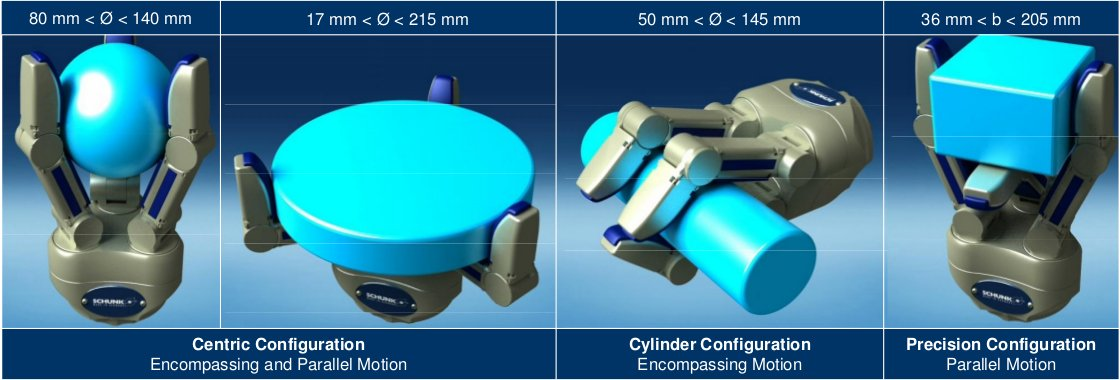
\includegraphics[width=1.0\textwidth]{images/grasp_types.jpg}
	\caption{Grasp types}
	{\scriptsize Image source: \cite{schunk2010}}
	\label{fig:grasp_types}
\end{figure}

\paragraph{SchunkHandController}

The \path{SchunkHandController} provides an implementation of the ROS interface for the Schunk gripper model. We designed this class to reflect the interface provided by the controller for the real hand. The basic topics are quite similar to those of the \path{LWRArmController}, as there are \path{joint_control/move} for setting joint target positions or \path{joint_control/get_state} for retrieving joint states. The controller allows to set the hand posture by setting target positions for all hand joints or based on different \emph{grasps} (figure \ref{fig:grasp_types}). \\

A grasp is defined by the parameters \emph{grasp type} and \emph{close ratio}. Allowed grasp types are \emph{cylindrical}, \emph{spherical}, \emph{centrical} and \emph{parallel}. The desired close ratio is defined as a value between 0 and 1. The controller calculates the corresponding joint positions, based on those parameters and sends the desired target positions to the underlying \path{SchunkHand}. Each grasp can be expressed, using three functions -- one for the position of the pivoting joints and the other two for the positions of the distal and proximal finger joints. The utilized functions were taken from the original controller code for the real hand. The definitions are listed in table \ref{fig:grasp_defs}. The first column holds the name of the grasp type. The second column shows how the positions of the pivoting joints are calculated. It can be seen that they are not influenced by the close ratio $x$ in all 4 grasp types. The third and fourth columns show the equations that are used to calculate the target values of the proximal and distal finger joints based on close ratio $x$. \\

The grasp strength can be adjusted, using the \path{settings/set_motor_current} topic. The message basically consists of a vector, holding a value for each joint that defines a percentage of the maximum motor strength. The real gripper also provides a topic that allows to read the current motor temperatures. For the sake of consistency, the \path{SchunkHandController} also provides this topic, but as V-Rep is not able to simulate motor heatings, only constant fake values are published. A complete interface description can be found in appendix \ref{app:sim_doc}.

\begin{table}[h]
  \centering
  \begin{tabular}{|l|c|c|c|} \hline
	\textbf{Name} & \textbf{pivoting} & \textbf{proximal} & \textbf{distal} \\ \hline
	CYLINDRICAL & $0$ & $(-30+30x)\frac{\pi}{180}$ & $(30 + 35x)\frac{\pi}{180}$ \\
	PARALLEL & $0$ & $(-75+82x)\frac{\pi}{180}$ & $(75-82x)\frac{\pi}{180}$ \\
	CENTRICAL & $\frac{\pi}{3}$ & $(-75+82x)\frac{\pi}{180}$ & $(75-82x)\frac{\pi}{180}$ \\
	SPHERICAL & $\frac{\pi}{3}$ & $(-40+25x)\frac{\pi}{180}$ & $(40+15x)\frac{\pi}{180}$ \\ \hline
  \end{tabular}
  \caption{Joint position functions based on close ratio $x$}
  \label{fig:grasp_defs}
\end{table}

\subsection{Publishing Kinect camera data}

The Kinect camera model does not contain any flexible parts that have to be controlled by the plugin. But it was necessary to make the images, captured by the simulated vision sensor available via ROS topics. This was achieved by using the corresponding functionality of the V-Rep default ROS interface that allows publishing vision sensor data, using the correct message types. Therefore we created a LUA script that is associated with the base element of the camera model within the simulation scene. This script simply extracts the object ID of the vision sensor and enables publishers for the captured RGB and depth images. The corresponding topics are \path{kinect1/sensoring/rgb_image} and \path{kinect1/sensoring/depth_image}. The script code can be seen in code listing \ref{lst:kinect}. Topic names can be changed within that script and the publishers can be dissabled by simply commenting the corresponding lines of code. The script also assigns the sensor data to an additional view within the simulation scene. This is helpful because it visualizes, the camera images during simulation.

\lstset{style=customc}
\begin{minipage}{\linewidth}
\lstinputlisting[caption={LUA script, attached to Kinect model}, label=lst:kinect]{code/kinect_script.lua}
\end{minipage} \\
% Motion planning first part
%!TEX root = thesis.tex

\chapter{Motion planning}
\label{chap:moveit}
This chapter explains the motion planning related part of the thesis. The introduction gives an overview about motion planning problems in general. Further on, the sampling based motion planning approach is described. Subsequent sections explain the integration of the motion planning framework \emph{MoveIt} into the existing robot setup.

\section{Introduction}

\citep[p. 1--11]{choset2005} describes motion planning as to be the task of finding a collision free path from one robot \emph{configuration} to another one. The classic path planning problem is the so called \emph{piano mover's problem}, originally mentioned by \cite{schwartz1983}. It is assumed to have a piano, which states a three dimensional rigid body and a set of known obstacles. The problem is to find a continuous motion that moves the piano from its current position to a given target position without touching any of the obstacles. Thereby the piano can freely be moved and rotated in Cartesian space. 

A generalized version of the \emph{piano mover's problem} is to find paths for a robot, composed from a set of rigid bodies, linked by joints while enforcing \emph{constraints} during that motions. A \emph{constraint} could be to avoid obstacles or to keep the robot's end effector in an upright position. Therefore it is important to have a representation of a robot's state that allows to determine the location of all robot parts. This representation is called the \emph{configuration} of a robot and the \emph{configuration space} is the set of all possible configurations, the robot is able to acquire. The dimension of the configuration space is the amount of \emph{degrees of freedom} (DOF), which is the number or independent variables that are necessary to describe a configuration. An imaginary free flying piano has six degrees of freedom as its configuration consists of the position and orientation $(x,y,z,roll,pitch,yaw)$ in Cartesian space. A robot arm with 7 joints has 7 degrees of freedom and its configuration are the joint positions. The motion planning problem is to find a path in the configuration space that connects start and goal configuration without violating constraints. This is a very complex problem and there exist various different approaches to find solutions. Examples are among others the \emph{bug algorithms}\citep[chapter 2]{choset2005}, \emph{potential functions}\citep[chapter 4]{choset2005} or \emph{sampling-based methods}\citep[chapter 7]{choset2005}. As the solution within this project only uses sampling based algorithms, a short overview about this class of methods will be given in the following section.

\section{Sampling-based motion planning}

Based on \citep[chapter 2]{omplPrimer}, sampling-based motion planning can be seen as a concept, capable of handling planning problems efficiently, especially for systems with many degrees of freedom. The general idea is to generate a set of random sample points that are uniformly distributed in the configuration space of the robot and then connect start and goal state by connecting the samples via collision free paths, with respect to possible motion constraints. Those methods are usually faster than traditional approaches because it is not necessary to reason about the whole configuration space but only about a finite number of sample configurations. The majority of sampling-based approaches are known to be \emph{probabilistic complete}, which means that the probability of finding an existing solution tends to 1 as the number of sample points increases to infinity. But they are not able to decide if a valid solution exists at all. The following definitions are used throughout this section to describe the concepts of sampling-based motion planning.

\begin{itemize}

\item \textbf{State space} \\
The \emph{state space} $\mathcal{S}$ is equal to the configuration space and consists of all possible robot configurations (states).

\item \textbf{Free state space} \\
The \emph{free state space} $\mathcal{S}_{free}$ is a subset of $\mathcal{S}$, containing only collision free states.  

\item \textbf{Path} \\
A \emph{path} is a sequence of states. If each state within the path is contained in $\mathcal{S}_{free}$, it is called a \emph{collision free} path.  

\end{itemize}

The sampling-based motion planners can be categorized into two major types - \emph{probabilistic roadmaps} (PRM) and \emph{tree-based planners}. Common to both methods is that they create uniformly distributed samples within the free state space. As the shape of $\mathcal{S}_{free}$ is not explicitly known, the created sample states are checked for collisions before using them. The following paragraphs give a short overview about both approaches.

\paragraph{Probabilistic roadmaps}

That approach uses the sampled states to create a ``roadmap'' of the free state space. Therefore each sample point is connected to an amount of $k$ nearby sample points via collision free paths. This is done by a local planner that simply interpolates between two points in the desired resolution while watching out for collisions. If no collision is detected, a new edge is introduced into the graph that is formed by the roadmap. After completing the graph, a planning query can be reduced to finding the shortest path within that graph that connects the start state and the goal state (figure \ref{fig:sampling_based}a).

\paragraph{Tree-based planners}

A lot of different sampling-based planning algorithm are using the tree based approach, as there are for example (RRT, EST, SBL or KPIECE). The difference to PRM is that this method uses a tree data structure of the free state space, which means that the resulting graph contains no cycles. The root of the tree is the start state and the tree is then expanded towards the goal state by creating collision free connections between sample points. If the goal is reached, the solution is found (figure \ref{fig:sampling_based}b). The different approaches differ in the strategy that is used to expand the tree towards the goal state.\\

\begin{figure}[ht]
	\centering
  	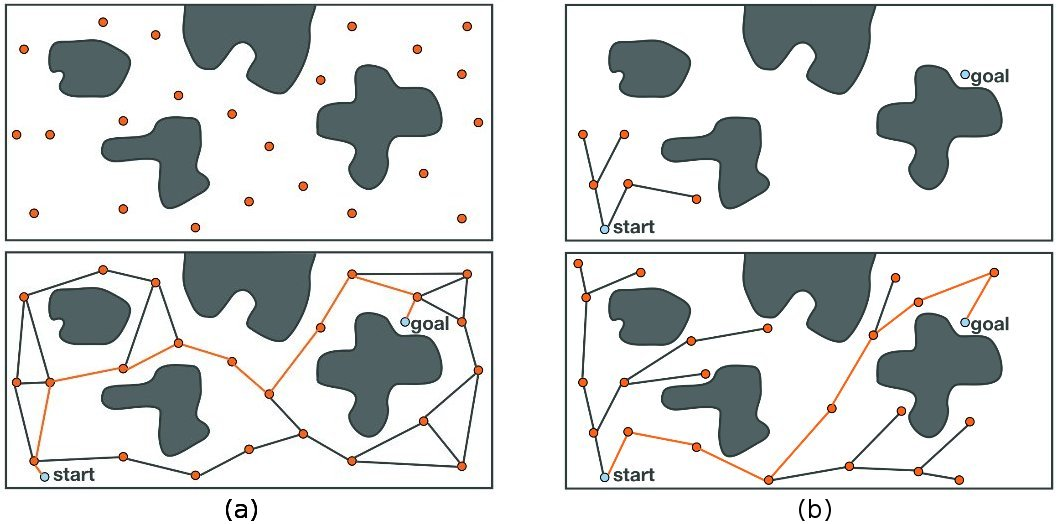
\includegraphics[width=1.0\textwidth]{images/sampling_based.jpg}
	\caption[Sampling based algorithms]{Probabilistic roadmap (left) and tree based approach (right)}
	{\scriptsize Image source: \citep{omplPrimer}}
	\label{fig:sampling_based}
\end{figure}

Generally can be said that the tree based approaches are more adequate for \emph{single query planning} because the tree usually does not has to cover the whole free state space. A roadmap could be reused for subsequent queries. As the most methods also require the search of a nearest neighbour, the utilized distance metric is also a crucial part within sampling-based motion planning as it is not always easy to identify the optimal method for finding nearby states in systems with large degrees of freedom.  

\section{The MoveIt motion planning framework}

\begin{figure}[ht]
	\centering
	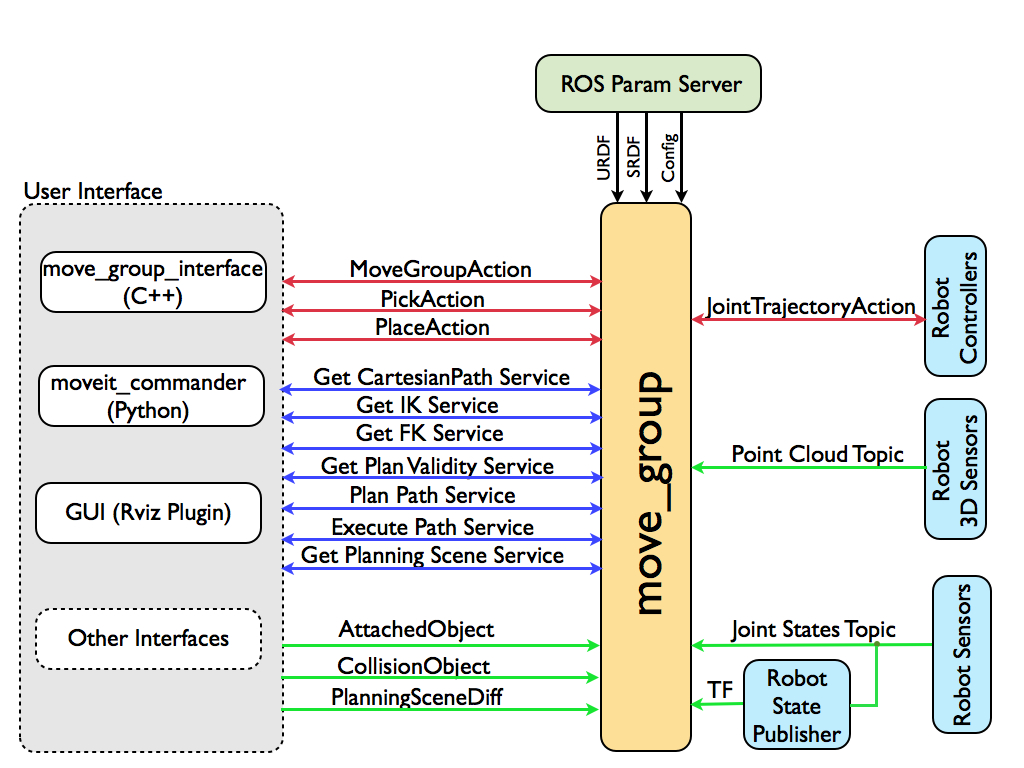
\includegraphics[width=0.75\textwidth]{images/moveit_architecture.jpg}
	\caption[Moveit architecture]{MoveIt architecture}
	{\scriptsize Image source: \url{http://moveit.ros.org/documentation/concepts}}
	\label{fig:moveit_arch}
\end{figure}

This section gives an overview about MoveIt's system architecture and introduces basic concepts. MoveIt\citep{MoveIt} is an open source framework for motion planning that is fully integrated into ROS. MoveIt was originally developed by Willowgarage\footnote{http://www.willowgarage.com} but since April 2012 it is maintained by the Open Source Robotics Foundation (OSRF). Figure \ref{fig:moveit_arch} gives an overview about the system architecture. \\

Central part of the framework is the \path{move_group} node. Configuration of that node happens via the parameter server. Therefore it is necessary to create a MoveIt configuration package. This is a ROS package that contains a description of the robot setup along with a number of necessary configuration files. The creation of that package and the necessary configuration steps are described in section \ref{sec:moveit_assistant}. The \path{move_group} node maintains a \emph{planning scene} which is an internal representation of the world. This planning scene bases on a kinematic description of the robot in the URDF format, which is a special markup language, designed to describe robots. The necessary steps to create that URDF description for our robot setup are explained in section \ref{sec:urdf}. \\

On top of this static description the \path{move_group} node needs to keep track of the current state of the robot. Therefore it expects the actual joint states to be published to a topic named \path{joint_states}. If there are additional objects within the robot's workspace that are not part of the robot description, they also have to be added to the planning scene. This can be done either by explicitly adding them via the corresponding topics (\path{CollisionObject} or \path{PlanningSceneDiff}) or by integrating information from 3D sensors like Kinect cameras. This information will then be taken into account during motion planning and collisions are avoided. But some collisions are intended. For example if an object has to be picked up, the gripper has to get in contact to this object. That means, collision checking for specific objects has to be (temporary) disabled to allow those controlled collisions. Therefore the \path{move_group} node maintains a so called \path{AllowedCollisionMatrix} to which objects can be added or removed. This also happens via the \path{PlanningSceneDiff} topic. \\

The \path{move_group} node provides a ROS interface, consisting of various ROS topics and services that allow to access its functionality. The services \path{GetIKService} and \path{GetFKService} can be used to solve inverse and forward\footnote{The problem of computing the end effector position in Cartesian space for a given robot configuration} kinematics problems. The \path{PlanPathService} handles motion planning requests and the \path{ExecutePathService} can be used to execute the planned trajectories on the connected hardware. Additionally there are the \path{PickAction} and \path{PlaceAction} servers available. Those action servers are intended to plan and execute all stages of pick and place operations. They were utilized in the benchmark pick and place task that was implemented in the scope of this project. Their usage is therefore described in chapter \ref{chap:pick_place}. \\

The functionality of the \path{move_group} node can be accessed in different ways. One way is to directly use the previously described services of the ROS interface. Another way is to use the \path{move_group_interface} which is a C++ wrapper around that ROS interface or the corresponding Python wrapper (\path{moveit_commander}). MoveIt also provides a planning plugin for the RViz visualization tool which can be used to do planning requests based on a graphical user interface. \\

The planning outcome of MoveIt is a time parametrized trajectory consisting of a set of waypoints. A waypoint is a joint configuration, described by the tuple $(p,v,a,t)$ where $p \in \mathbb{R}^n$ are the positions, $v \in \mathbb{R}^n$ the velocities and $a \in \mathbb{R}^n$ the accelerations at time $t$ and $n$ is the number of involved joints. Those waypoints mark the important points along the path, the manipulator has to move. Connecting  MoveIt to the hardware requires therefore controllers that are able to translate such time parametrized trajectories into a sequence of suitable motor commands. Just sending the joint positions within the waypoints to the robot would not suffice as a trajectory is also constrained in terms of \emph{velocities} and \emph{accelerations} over \emph{time}. Therefore the controller needs to be able to interpolate between the subsequent waypoints and calculate intermediate joint positions based on the loop rate of the control cycle. Section \ref{sec:hardware_adapter} explains in detail how this problem was solved and how the connection to the (simulated or real) hardware was established.\\

Various important parts of MoveIt are implemented as plugins which means they are replaceable by other components that provide the same interface. The inverse kinematics plugin we utilized uses the Kinematics and Dynamics Library\footnote{http://www.orocos.org/kdl} (KDL) for solving IK problems. The planning plugin provides access to the sampling based planners of the  Open Motion Planning Library\footnote{http://ompl.kavrakilab.org} (OMPL), which is a framework that contains implementations of many different motion planning algorithms. Therefore it is possible to choose, which one of those algorithms to use during planning requests. \\

\section{Creating the URDF model of the robot setup}
\label{sec:urdf}

The \emph{Unified Robot Description Format} (URDF) is a markup language, designed to describe robots. The description happens in text files, in a special XML format. The most important elements in the XML specification\footnote{http://wiki.ros.org/urdf/XML} are:

\begin{itemize}

\item \textbf{link} \\
Describes the all necessary properties of a specific robot link. Each link must have a unique name. The visual, inertial and collision details are configured in the corresponding subtags of the link element. The visual part as well as the collision model can either be composed from primitive shapes
or from mesh files. If mesh files are used it is important that they are not to complex. Especially for the collision model it is recommended to use a simplified model to avoid a performance loss because during planning requests there happens a lot of collision checking.

\item \textbf{joint} \\
Describes the properties of a joint. A joint is a flexible connection between two links, having exactly one parent and one child link. Each joint states a new reference frame for its child link and it is positioned relative to its parent frame. The joint actuates its child link relative to its parent link along the joint axis. There are different types of joints available but for the current project only \emph{fixed} and \emph{revolute} joints are of interest. A fixed joint states a rigid connection between parent and child link. A revolute joint is a rotational joint with one degree of freedom. Details like angular joint limits, axis orientation and the dynamic properties of the joint motors can be configured in the corresponding subtags of the joint element.

\end{itemize}
\begin{figure}[ht]
	\centering
  	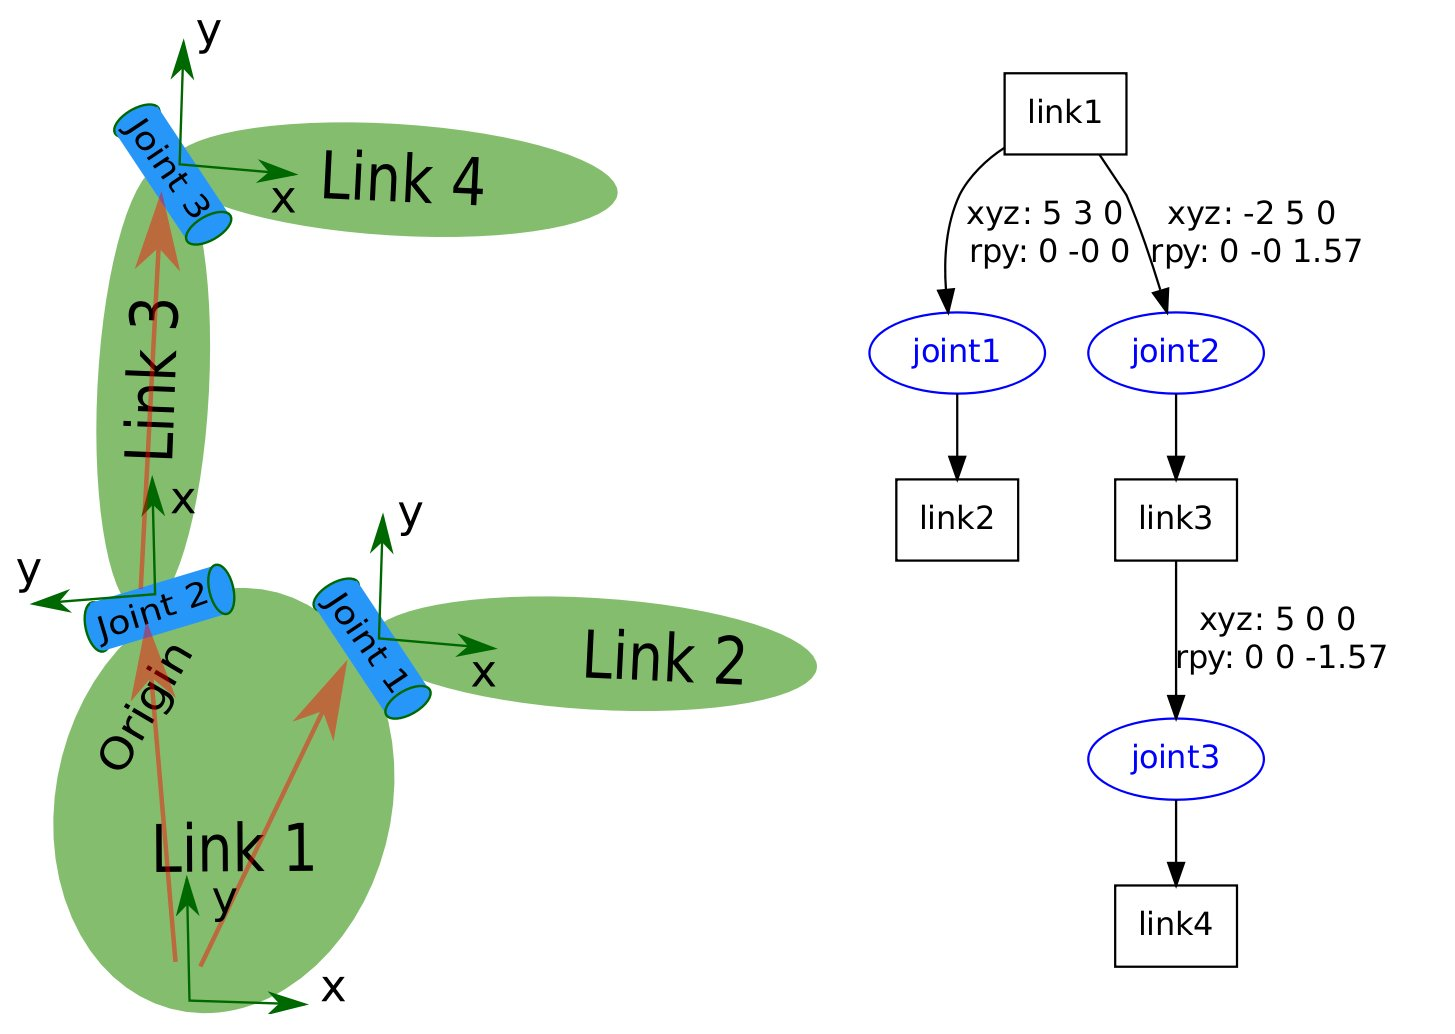
\includegraphics[width=0.75\textwidth]{images/urdf_chain.jpg}
	\caption[URDF graph]{URDF graph}
	{\scriptsize Image source: http://wiki.ros.org/urdf/Tutorials/Create your own urdf file}
	\label{fig:urdf_graph}
\end{figure}
Those elements are used to form the URDF graph that exactly describes the kinematic chain of the robot components and their placement relative to each other. A simple example for such a graph is visualized in figure \ref{fig:urdf_graph}. This description can get very large as a lot of different components are involved. So it is possible to organize it into a set of text files, each one describing one part of the whole. For example one file could describes a robot arm. Other files can then use that description and insert multiple instances of that arm into the setup. The \texttt{xacro} ROS package provides the necessary functionality to combine all those text files into one XML string. \emph{XACRO} stands for \emph{XML Macro} and is designed to parse xacro files and combine them into one single XML document, containing the resulting URDF description.\\

The URDF description of the IIS robot setup is spread across multiple packages, located in the \path{iis_hardware} directory of the \path{iis_robot_sw} repository. Arm and gripper descriptions are located in seperate packages (\path{lwr_description} and \path{schunk_description}), the \path{iis_robot} package brings all the components together. The description of the Schunk SDH gripper was taken from the \path{schunk_description} ROS package. The model of the KUKA LWR arm was adapted from the Github repository\footnote{https://github.com/RCPRG-ros-pkg/lwr\_robot/tree/hydro-devel/lwr\_defs} of the \emph{Robot Control and Pattern Recognition Group}\footnote{University of Warsaw (http://robotyka.ia.pw.edu.pl/twiki/bin/view/Main)}. The other parts of the model, namely the robot torso and the table had to be created. The descriptions are located in a seperate files within the \texttt{uibk\_robot} package (\texttt{torso.xacro} and \texttt{table.xacro}). \\

\begin{figure}[h]
	\centering
  	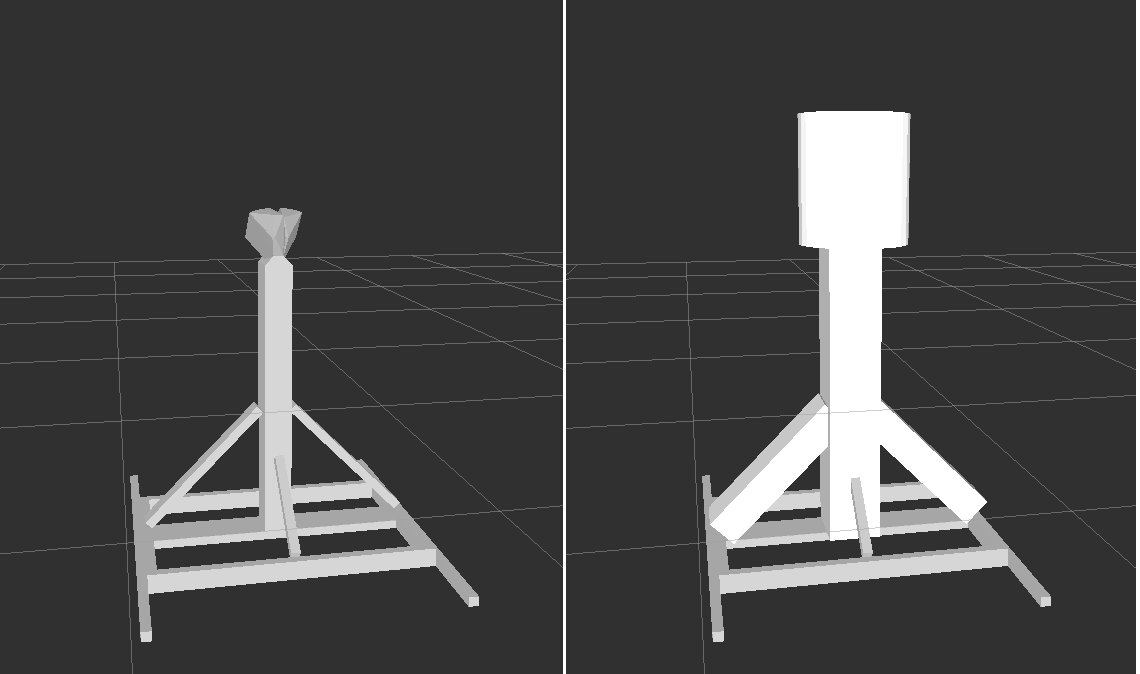
\includegraphics[width=1.0\textwidth]{images/torso.jpg}
	\caption{Visual and collidable model of torso}
	\label{fig:torso_col}
\end{figure}

The mesh files, used in the description of the robot torso have been exported from the V-Rep simulation scene. For the visual part we took the mesh as it is. For the collision geometry we created an increased version of the original mesh to provide a safety padding of 2.5 cm around the torso links. Moreover a cylinder with a diameter of 40 cm was added in the head area to ensure that the planner avoids accidental hits in the region where the Kinect camera is mounted. Figure \ref{fig:torso_col} shows the visual (left image) and the collidable (right image) part of the torso model. \\

The table was modelled from primitive shapes. We designed the XML structure of the table description in a way that allows to easily adjust the size of the table, as can bee seen in listing \ref{lst:table}. The collision geometry of the table is also slightly larger than the visual part to provide safety margins. \\

\lstset{language=XML,style=customxml}
\begin{minipage}{\linewidth}
\begin{lstlisting}[caption={XML snippet, inserting the table model into the URDF}, label=lst:table]
<!-- draw the table relative to the origin -->
<xacro:model_table name="table" 
	     parent="world"
	     length="2.22"
	     width="0.8">
	<!-- Place the table relative to the world reference frame -->
	<origin xyz="-0.029 -0.3 0" />
    
</xacro:model_table>
\end{lstlisting}
\end{minipage}

After attaching the two grippers to the arms it showed that the offset between gripper wrist and last arm link was not correct. To correct that issue the file \texttt{sdh\_with\_connector.xacro} was created which simply places an additional ring between the last arm link and the gripper to achieve the correct offset. The content of that file is listed in \ref{lst:urdf_sdh} \\

The file \path{iis_robot_table.xacro} draws all the pieces together. It describes the whole setup, consisting of the torso, two arms, two grippers and the table. The root element of the model hierarchy is a link called \texttt{world\_link}. Torso, table and both arms are positioned relative to that root link. Therefore we used the same transformations as for the simulation model. Changing the origin of the world reference frame could easily be achieved by shifting the root link to a new position. Figure \ref{fig:robot_table} shows a visualization of the resulting robot description. The complete listing of the \path{iis_robot_table.xacro} file can be found in listing \ref{lst:urdf_robot_table}.

\begin{figure}
	\centering
  	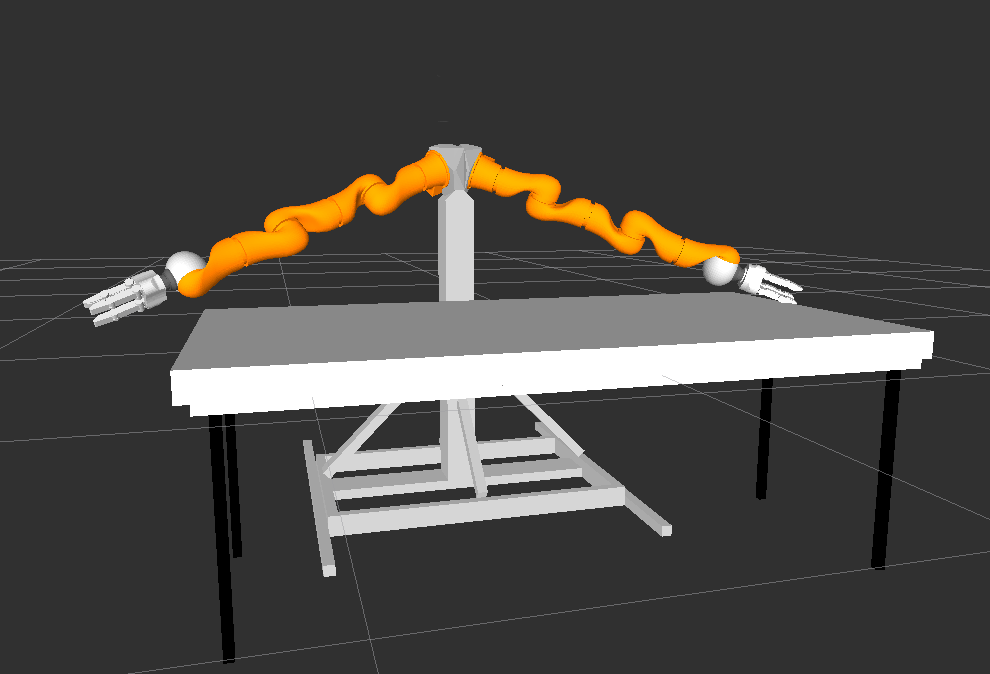
\includegraphics[width=0.75\textwidth]{images/iis_robot_table.png}
	\caption{URDF description in RViz}
	\label{fig:robot_table}
\end{figure}

\section{Creating the MoveIt configuration package}
\label{sec:moveit_assistant}

After designing the URDF description of our robot setup it was necessary to create a MoveIt configuration package. This was done, using the \emph{MoveIt Setup Assistant} which is part of the MoveIt distribution. This software tool provides a graphical user interface that allows to configure and generate a ROS package that contains all necessary MoveIt configuration files based on an existing URDF model. This section explains the steps that had to be performed and the resulting configuration package. \\ 

The Setup Assistant was launched using the following command line statement:
\begin{quote}
\begin{verbatim}
roslaunch moveit_setup_assistant setup_assistant.launch
\end{verbatim}
\end{quote}
This command brings up the Setup Assistant which asks for the file path to the previously created URDF description. After pointing the Setup Assistant to the correct file location, we had to perform the following configuration steps:

\begin{itemize}

\item \textbf{Computing the self collision matrix}

The \emph{self collision matrix} consists of pairs of robot links that can safely be excluded from collision checking. Adjacent links of the robot arm for example are in permanent collision. Collisions between other links can never happen because they are simply too far apart. The Setup Assistant can be triggered to compute this self collision matrix automatically by testing a large number of different robot configurations while tracking for link pairs that are hardly always in collision and pairs that are never in collision. The number of sample configurations to check can be adjusted. We selected the maximum possible density of 100.000 sample configurations to find as many colliding link pairs as possible. This is important because excluding a large number of link pairs raises performance during motion planning because collision checking is an expensive process. The resulting self collision matrix can be adjusted manually if necessary. The image in figure \ref{fig:self_col} shows a screenshot of this configuration step.

\begin{figure}[p]
	\centering
  	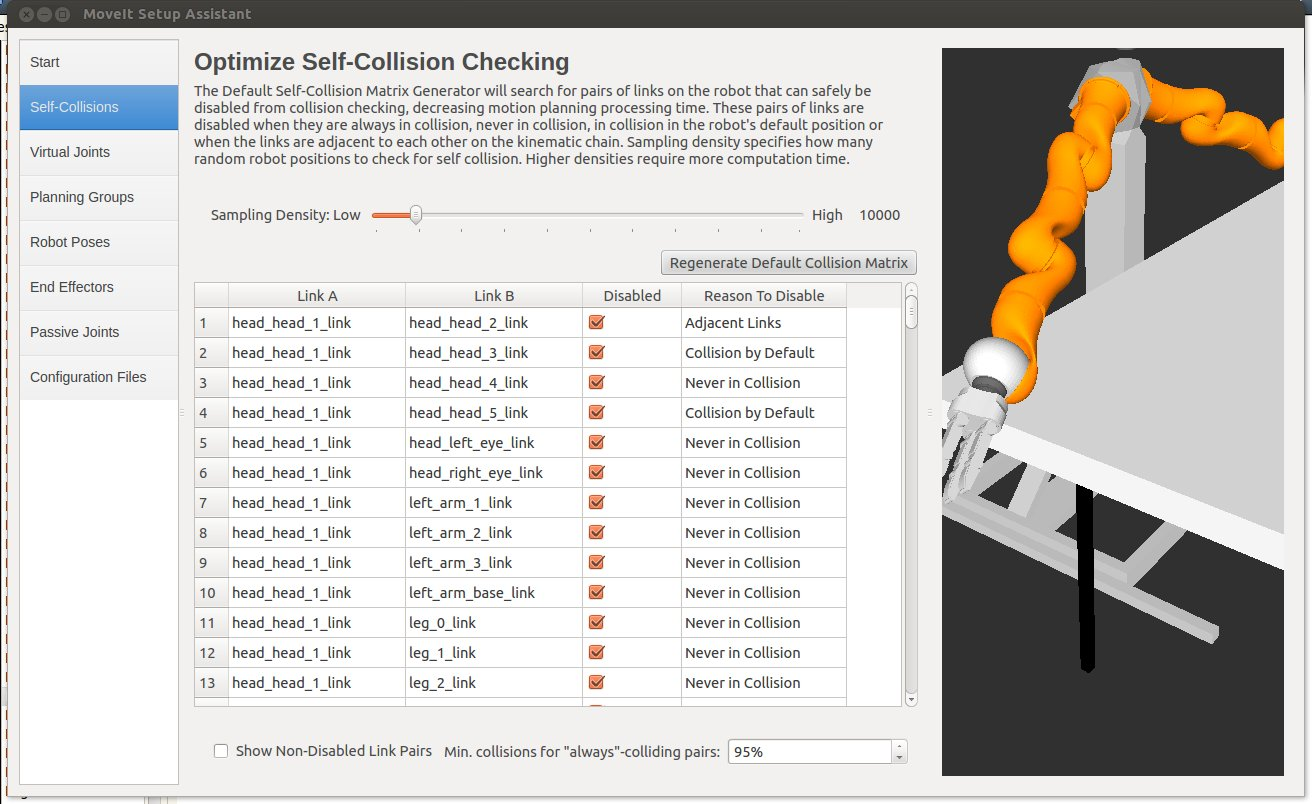
\includegraphics[width=0.75\textwidth]{images/self_collision.jpg}
	\caption{Computing the self collision matrix}
	\label{fig:self_col}
\end{figure}

\item \textbf{Defining the planning groups}

MoveIt requires to define so called \emph{planning groups} for the robot setup. A planning group is a group of links and joints within the model that can be seen as a logical component, e.g. a gripper or a robot arm. Each planning group consists of a unique name and a list of robot links and joints that are part of that group. Additionally can be specified, which IK solver should be used for the planning group.Each planning request in MoveIt is done against one of those defined planning groups. We defined planning groups for the both arms (\path{left_arm} and \path{right_arm}) and grippers (\path{left_sdh} and \path{right_sdh}). We decided to use the default KDL solver for the arms. An additional planning group, called \path{both_arms} was created that allows planning requests for both robot arms simultaneously. They were defined on the \emph{Planning Groups} page of the Setup Assistant (figure \ref{fig:planning_groups}).

\begin{figure}[p]
	\centering
  	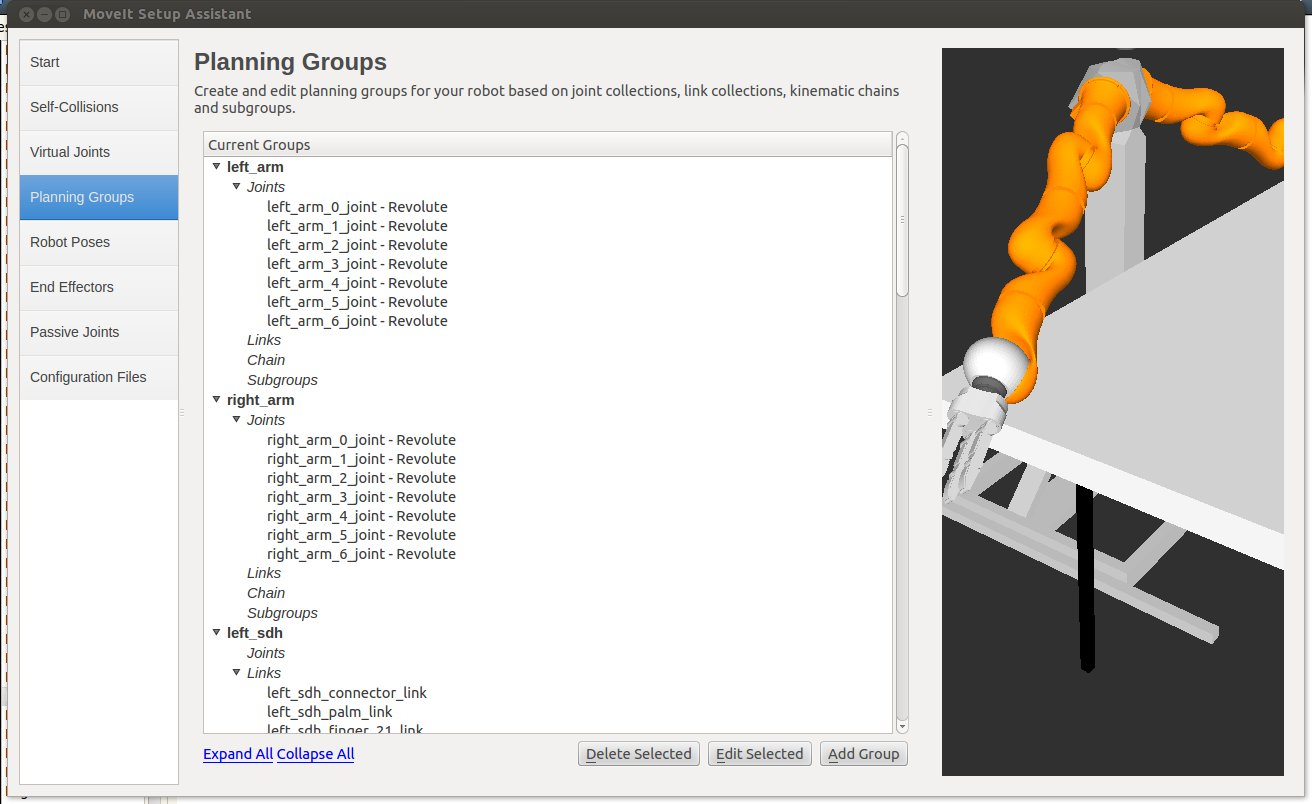
\includegraphics[width=0.75\textwidth]{images/planning_groups.jpg}
	\caption{Defining planning groups}
	\label{fig:planning_groups}
\end{figure}

\item \textbf{Defining the end effectors}

Each planning request in MoveIt requires to specify the end effector of the selected planning group. Those end effectors also had to be defined during the setup process. An end effector definition in MoveIt consists of a unique name, the underlying planning group (e.g. \path{left_sdh} or \path{right_sdh}), the parent planning group (e.g. \path{left_arm} or \path{right_arm}) and the name of the last link in the kinematic chain of the parent group. We defined end effectors as listed in table \ref{tbl:eef_defs}, using the \emph{End Effectors} page of the Setup Assistant.

\begin{table}[h]
  \centering
  \begin{tabular}[h]{|l|l|l|l|} \hline
	\textbf{Name} & \textbf{EEF group} & \textbf{Parent group} & \textbf{Parent link} \\ \hline
	\path{left_eef} & \path{left_sdh} & \path{left_arm} & \path{left_arm_7_link} \\
	\path{right_eef} & \path{right_sdh} & \path{right_arm} & \path{right_arm_7_link} \\ \hline
  \end{tabular}
  \caption{End effector definitions}
  \label{tbl:eef_defs}
\end{table}

\item \textbf{Completing the Setup Assistant}

The last step in the setup process was to generate a MoveIt configuration package based on the previously explained configuration steps. Therefore the Setup Assistant required to specify the desired package name which we set to \path{uibk_robot_moveit_config}. After triggering the package generation on the \emph{Configuration Files} page of the Setup Assistant, the resulting ROS package was created at the specified save location. 
 
\end{itemize}

The package that was generated during this setup process contains all the configuration and launch files that are necessary to make planning requests for our robot setup though it is not yet connected to the hardware. The configuration can be tested by running it in demo mode. This mode allows to plan and execute trajectories without being connected to the robot hardware. The demo mode is launched with the following command line statement:
\begin{quote}
\begin{verbatim}
roslaunch uibk_robot_moveit_config demo.launch
\end{verbatim}
\end{quote}
This command runs a \path{move_group} node using the previously created configuration and starts an instance of RViz with the motion planning plugin. There it is possible to switch between planning groups, set start and target configurations, do planning requests and visualize the resulting trajectories based on a graphical user interface. \\

The launch files within the configuration package are responsible for uploading the configuration parameters to the parameter server and start the \path{move_group} node. Those parameters are defined in several configuration files, located in the \path{config} folder of the configuration package. The following paragraphs just give an overview about content of the most important files. Detailed information can be found in the MoveIt documentation\footnote{http://moveit.ros.org/documentation/concepts/}.

\paragraph{\texttt{controllers.yaml}}
The content of this file specifies the available controllers for the (simulated or real) hardware. The file is initially empty and has to be populated manually. This was done after implementing the required controller interface, which is described in section \ref{sec:hardware_adapter}.

\paragraph{\texttt{fake\_controllers.yaml}}
This file is populated by the Setup Assistant and contains the definitions for the \emph{fake} controllers. The fake controllers simulate a connection to the hardware by providing the required ROS interface. They are used in demo mode to visualize the commanded robot motions in RViz. Each fake controller is defined by its name and a list, containing the names of the controlled robot joints.

\paragraph{\texttt{iis\_robot.srdf}}
This file contains all the semantic information about the robot that was configured during the setup process. The content is specified using the SRDF\footnote{http://wiki.ros.org/srdf} format. It holds the definitions of the configured planning groups, end effectors and the generated self collision matrix entries.

\paragraph{\texttt{joint\_limits.yaml}}
This file holds the velocity and acceleration limits of all joints contained in the robot description. The Setup Assistant creates the initial values based on the URDF model but this configuration file allows to specify other limits if necessary. MoveIt uses the limits that are configured within this file, not those configured in the URDF description. We used that option to drastically reduce the maximum allowed velocity of all arm joints to achieve slower robot motions.

\paragraph{\texttt{kinematics.yaml}}
This file contains the definition of the IK solvers that should be utilized for the robot arms. Currently we use the KDL kinematics plugin that is part of the MoveIt distribution. Additional parameters specify the default timeout value that is used for each IK calculation attempt and the maximum amount of iterations.

\paragraph{\texttt{ompl\_planning.yaml}}
This file holds OMPL specific configuration parameters. It defines the allowed planning algorithms for each planning group. We left the content of that file at its default values. \\

The configuration of this package can be adjusted either by editing the configuration files manually or by launching the Setup Assistant again. This can be done, using the \path{setup_assistant.launch} file from this package.

\section{Connecting MoveIt to the existing robot control interface}
\label{sec:hardware_adapter}

After creating the configuration package it was necessary to find a way to connect MoveIt to the (simulated or real) hardware to allow the execution of the planned trajectories. This section explains the necessary steps in detail. \\

The connection to the hardware happens via the \path{FollowJointTrajectory} action interface. This is a special kind of ROS interface that builds upon the \emph{ROS action protocol}\footnote{http://wiki.ros.org/actionlib/DetailedDescription}. Each robot component that is intended to be controlled by MoveIt has to provide this interface. The interface comprises of the following topics:
\begin{itemize}

\item \path{follow_joint_trajectory/goal}

This topic is used to send a \path{FollowJointTrajectoryActionGoal} message to the controller. This message describes a time parametrized trajectory that has to be executed along with allowed tolerance values for final joint positions and execution time. Those tolerances specify how precise the controller has to stick to the position, velocity, acceleration and time constraints defined for the trajectory in order to consider the execution to be successful.

\item \path{follow_joint_trajectory/feedback}

The controller uses this topic to continuously provide feedback about the current execution status. The feedback message contains information about the trajectory point the controller is currently processing.

\item \path{follow_joint_trajectory/result}

After finishing the trajectory execution the controller publishes the result to this topic. If the final joint positions lie within the specified tolerance values and the time constraints were met, the trajectory execution is considered to be successful. The message contains a status code and a status message.

\end{itemize}
The existing control interface of the robot components only allows to send joint target positions to the \path{joint_control/move} topic but without any time parametrization. So it was necessary to implement an additional ROS node that is capable of executing the generated trajectories, using the existing infrastructure. Therefore we utilized the functionality of the \path{ros_control} stack\footnote{http://wiki.ros.org/ros\_control}. Those packages allow to integrate and control robot hardware in a generalized way, facilitating the usage of existing controllers on different robots. The following section gives an overview about the \path{ros_control} stack.

\subsection{ROS control stack overview}

\begin{figure}[h]
	\centering
  	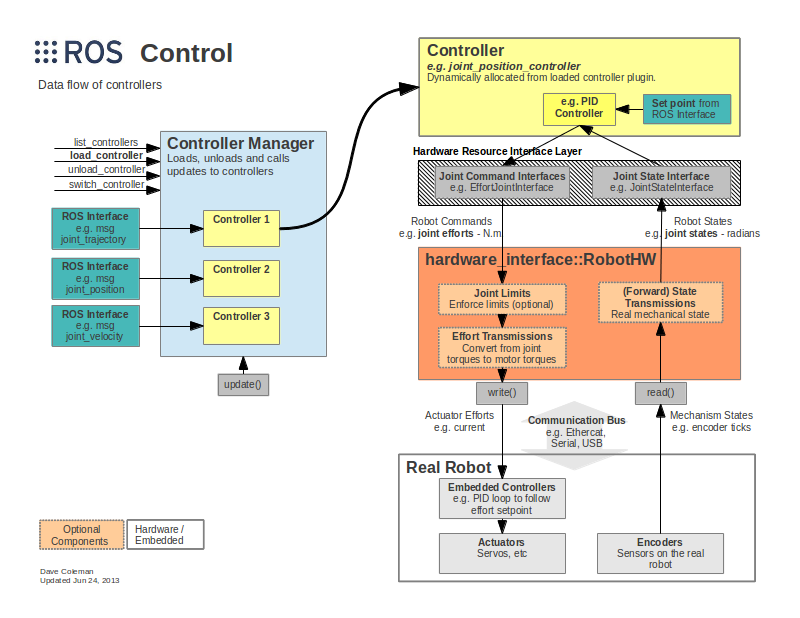
\includegraphics[width=1.0\textwidth]{images/ros_control.png}
	\caption{ROS control architecture}
	{\scriptsize Image source: http://wiki.ros.org/ros\_control}
	\label{fig:ros_control}
\end{figure}

A controller provides a ROS interface and translates the incoming control commands into suitable hardware commands. The ROS interface is controller specific and depends on how the robot is used. MoveIt for example requires controllers that provide the \path{FollowJointTrajectory} action interface, as explained above. The structure of the hardware commands depend on the available connection to the robot hardware. Some robots require commands that specify the target effort for the joint motors. Others, like our robot components allow to set joint target positions. The controllers are operated in a control loop which should run in real time. On each iteration of this control cycle the current state of the hardware is read. Then the controller calculates the control commands, based on the current state and the time since the last iteration. After that, the commanded values are sent back to the hardware and the next iteration starts. \\

Figure \ref{fig:ros_control} shows an overview about the \path{ros_control} architecture. The \path{ros_control} stack contains implementations for different kinds of generic hardware controllers. Within this project we utilized several \path{JointTrajectoryControllers}. This controller provides the \path{FollowJointTrajectory} action interface and calculates an interpolation between the trajectory waypoints that satisfies the velocity, acceleration and time constraints of the planned trajectory. The result are intermediate joint positions for each iteration of the control cycle that can be sent as target positions to the robot. The controller reads current hardware state like joint positions and velocities via the \path{JointStateInterface}. For writing the commanded values, the controller requires a \path{PositionJointInterface}. This interface simply allows to set a target position for a joint with a given name. Those interfaces are provided by the abstract \path{RobotHW} class which represents the connection to the hardware. Inheriting classes that represent a concrete robot have to register all the robot joints by their names (as configured in the URDF description), maintain their states and send commanded values back to the concrete hardware. \\

The controllers need to be registered on a \path{ControllerManager} instance. This class holds a reference to a \path{RobotHW} instance and provides an interface composed from ROS services that allows to load and start controllers for the connected hardware. The \path{LoadController} service forces a \path{ControllerManager} to load a controller with given name. It is necessary that a configuration for that controller is available on the parameter server that specifies the concrete controller type and controller specific details. After loading the controller it also needs to be started. This is done, using the corresponding \path{StartController} service. During the control cycle, the \path{ControllerManager} is responsible for updating all active controllers. \\

\subsection{Designing the hardware adapter node}

\begin{figure}[h]
	\centering
  	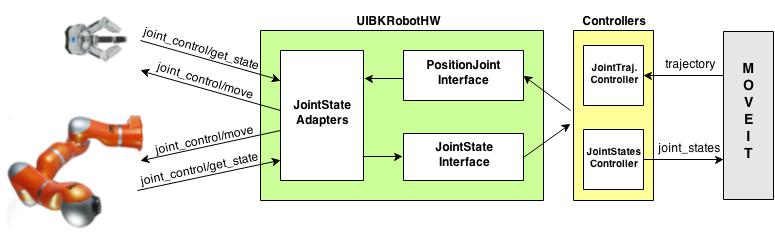
\includegraphics[width=1.0\textwidth]{images/hardware_adapter.jpg}
	\caption{Hardware adapter architecture}
	\label{fig:hardware_adapter}
\end{figure}

The \emph{hardware adapter} is an independent ROS node that we implemented to act as connection between MoveIt and the simulated or real hardware. The code and necessary configuration and launch files are located in the \path{uibk_moveit_adapter} package. The solution provides the necessary infrastructure for using generic controllers from the \path{ros_control} packages. Figure \ref{fig:hardware_adapter} gives an overview about the hardware adapter architecture. The \path{UibkRobotHW} is a subclass of \path{RobotHW} and represents the connection to the robot. It maintains the complete state of all joints in the connected robot components. Joints are represented by the \path{Joint} datatype, consisting of a unique joint name, state parameters and a commanded target position. For controllers, the \path{UibkRobotHW} class provides a \path{JointStatesInterface} and a \path{PositionJointInterface}. Active controllers use those interfaces to access the current state and for commanding target positions. \\ 

The \path{UibkRobotHW} utilizes a set of \path{JointStateAdapters}. A \path{JointStateAdapter} represents the connection to one specific robot component, e.g. a robot arm or a gripper. During the control cycle the \path{JointStateAdapters} read current joint states from the appropriate topics and send commanded values back to the hardware. Our solution allows to configure the utilized topic names via the parameter server.\\

On hardware adapter startup, an instance of the \path{UibkRobotHW} class is created and initialized by using the corresponding class method. It then searches the parameter server for the a parameter named \path{hardware_adapter/adapter_list}. This parameter specifies the names of the \path{JointStateAdapters} that need to be created. The \path{UibkRobotHW} class then creates a \path{JointStateAdapter} instance for each name it finds in the configured adapter list, based on the provided configuration settings. Listing \ref{lst:adapter_config} shows the current content of the corresponding configuration file (\path{adapter_config.yaml}). As the names of the topics that are used by the \path{JointStateAdapters} can be configured it becomes clear that the hardware adapter is able to interact with the simulator and the real robot as well, as both of them provide exactly the same ROS interface just within different namespaces. Available configuration parameters are:

\begin{itemize}

\item \textbf{\path{adapter_list}} \\
Contains a list of all \path{JointStatesAdapters} that have to be created. For each adapter name mentioned in this list a detailed configuration is required. The subsequent parameters have to be configured for each single adapter.

\item \textbf{\path{joint_state_topic}} \\
The name of the topic where a specific adapter listens for joint states. The expected message type  \path{sensor_msgs/JointStates}. This parameter is mandatory.

\item \textbf{\path{readonly}} \\
This parameter is optional. If true then the adapter will only listen for joint states but not publish commanded values.

\item \textbf{\path{joint_command_topic}} \\
The name of the topic the adapter should use to publish the commanded values to. The expected message type is \path{std_msgs/Float64MultiArray}. This parameter is mandatory if the adapter is not configured to be read only.

\item \textbf{\path{joints}} \\
A list of joint names that should be controlled by the adapter. The order in this list also determines the order of the values in the published message.

\item \textbf{\path{joint_name_prefix}} \\
This parameter can be used to be able to uniquely identify joints. For example both arms are using the same joint names (\path{arm_0_joint}, \path{arm_1_joint},\ldots). But in a URDF model, joint names have to be globally unique. Therefore the prefix can be used to prepend the original name to achieve uniqueness. A prefix value of \path{right_} for example will lead to the joint names \path{right_arm_0_joint}, \path{right_arm_1_joint},\ldots).

\end{itemize}

After instantiation, each \path{JointStateAdapter} waits a certain amount of time for a message containing the initial joint states on its configured joint states topic. If it does not receive such a message before timeout, it will automatically shut down for safety reasons and report an error. This is very important as the \path{JointStateAdapter} imediately begins to send joint positions after initialization. The position to be sent is initially the currently known position, as long as no other values have been commanded by the controllers. Therefore the initial position always has to be known, otherwise dangerous and rapid robot motions could occur on startup.

\begin{minipage}{\linewidth}
\lstinputlisting[caption={JointStateAdapter configuration}, label=lst:adapter_config]{code/adapter_config.yaml}
\end{minipage} \\

After the previously described initialization process a \path{ControllerManager} instance is created and the control loop is started. As the control loop must not be interrupted by ROS callback functions, it is launched in a separate thread. On each iteration the exact time since the last step is calculated. The \path{ControllerManager} is then forced to update all active controllers based on the time since last iteration. After handling the controllers, \path{JointStatesAdapters} are forced to send the commanded values to the hardware. This is done using the \path{publish} function of the \path{UibkRobotHW} class. Listing \ref{lst:control_loop} shows the code of the control loop thread.

\begin{minipage}{\linewidth}
\lstinputlisting[caption={Control loop thread}, label=lst:control_loop, style=customc]{code/control_loop.cpp}
\end{minipage} \\

It is important to note, that a running hardware adapter instance only provides the necessary infrastructure for \emph{using} controllers of the \path{ros_control} packages, not the controllers themselves. The required controllers still have to be loaded and started, using the corresponding ROS services of the \path{ControllerManager}. This has to be done after starting an instance of the hardware adapter node.

\subsection{Launching the hardware adapter}
\label{sec:launch_moveit}

This section describes how hardware adapter instances are launched for the simulator and the real robot, along with the arm and gripper controllers. \\

The file \path{hardware_adapter.launch}, located in the \path{uibk_moveit_adapter} package was created to handle the necessary configuration parameter upload and launch the hardware adapter node for the simulator and the real robot as well. As can be seen in listing \ref{lst:adapter_config} are the configured topic names for the \path{JointStateAdapters} defined, using \emph{relative} topic names (i.e. without trailing slash). The required instance is than accessed by simply shifting the node into \path{simulation} or \path{real} namespace. This is realized, specifying the \path{config_name} parameter of the launch file. The following command line statement launches a hardware adapter instance for the \path{simulation} namespace:
\begin{verbatim}
roslaunch uibk_moveit_adapter hardware_adapter.launch config_name:=simulation
\end{verbatim}

\lstinputlisting[caption={Launching the hardware adapter (\texttt{hardware\_adapter.launch})}, label=lst:adapter_launch]{code/hardware_adapter.launch}

Listing \ref{lst:adapter_launch} shows the content of this launch file. The \path{ns} argument of the \path{<group>} tag specifies the namespace for all nodes that are launched within that group. That means all relative topic names are prepended with the namespace, defined in the \path{config_name} attribute. A relative topic name of \path{left_arm/joint_control/move} for example results in the absolute topic name \path{/simulation/left_arm/joint_control/move}.\\

The controller configurations are located in separate files, namely \path{arm_controllers.yaml} and \path{gripper_controllers.yaml}. Listing \ref{lst:arm_controller} shows the controller configuration for the left and the right arm. The \path{type} parameter specifies the controller type. The \path{joints} parameter contains the names of the robot joints, the controller is responsible for. The section \path{constraints} describes controller specific tolerance values. The \path{goal_time} value defines the amount of time the controller is allowed to exceed the trajectory execution time to still consider the execution to be successful.

\lstinputlisting[caption={Configuration of arm controllers (\texttt{arm\_controllers.yaml})}, label=lst:arm_controller]{code/arm_controllers.yaml}

The launch file \path{controllers.launch} is responsible for uploading those configuration files to the parameter server and run the controllers. Listing \ref{lst:controllers} shows the content of this file. After uploading the content of the configuration files, all the controllers are loaded and started.
Utilized controllers are the previously described \path{JointTrajectoryController} and the \path{JointStateController}. The \path{JointStateController} publishes the collected states of all robot joints at once to the \path{joint_states} topic, which is used by the \path{move_group} node to monitor the current state of the robot. \\

\lstinputlisting[caption={Launching controllers (\texttt{controllers.launch})}, label=lst:controllers, style=customxml]{code/controllers.launch}

After a successful hardware adapter startup all the required controllers are available. The node provides feedback information about the state and errors during the startup process on the console output. It is crucial that the joint state topics of simulator or real robot are available before launching the hardware adapter node, otherwise it will not be able to work because of missing initial joint states. After successful startup, the additional controller topics can be found in the corresponding namespace.

\section{Adjusting the MoveIt configuration}

The prerequisites were now made for connecting MoveIt to the (simulated or real) robot. The last remaining step was to adjust the MoveIt configuration for establishing a connection to the \path{FollowJointTrajectory} controllers. Therefore we modified the configuration file \path{controllers.yaml} in the \path{uibk_robot_moveit_config} package. It contains a list, describing the controllers that are made available by the hardware adapter. Each controller description contains the name of the controller, its namespace, the controller type and a list, containing the names of the controlled joints.\\

For starting MoveIt we created the launch file \path{moveit_planning_execution.launch}. The aim of this file is to launch a fully configured \path{move_group} node either for simulated or real robot, together with the corresponding hardware adapter. The namespace can be selected using a boolean parameter named \path{simulation}. The following statement launches a MoveIt configuration, connecting the \path{move_group} instance to the real robot.
{\small 
\begin{verbatim}
roslaunch uibk_robot_moveit_config moveit_planning_execution.launch simulation:=false
\end{verbatim}}
The launch file also starts the RViz visualization tool configured with the motion planning plugin. This is used for visualizing the planned trajectories and can also be used to test the connection to the robot by making planning requests and execute the resulting trajectories.

\section{Testing the IK solver}

Solving the inverse kinematics problem is an important issue when working with the robot arms. Many planning algorithms depend on an IK solution for a given Cartesian space goal before they are able to solve planning problems. So we decided to test the quality of the KDL inverse kinematics solver that is used by MoveIt. As a side effect we were able to use the test results to visualize the area in the robot workspace that can be reached by the robot the arms. \\

\begin{table}[h]
  \centering
  \begin{tabular}[h]{|l|c|c|c|} \hline
	\textbf{Arm} & \textbf{Redundant IK} & \textbf{KDL solver} & \textbf{\%} \\ \hline
	Left arm & $10.392$ & $15.474$ & $+48.9$ \\
	Right arm & $10.025$ & $15.444$ & $+54.0$ \\ \hline
  \end{tabular}
  \caption{IK test results}
  \label{tbl:ik_results}
\end{table}

First we computed a test set, composed from 3.500 sample locations within the robot workspace. The sample points are uniformly distributed throughout the area that should be reachable by at least one of the robot arms. The offset between the samples is 10 cm in $x$, $y$ and $z$ direction. For each sample point we computed 17 different orientations. That resulted in a set, containing 59.500 sample poses. During testing we assumed those test poses to be end effector target positions. The test utilized MoveIt's IK functionality (KDL) to compute a valid joint configuration for each single sample pose and counted the positive results. This was done for each arm separately. The outcome was a set of sample poses, the solver was able to find valid solutions for. The same test was repeated, using the pre-existing IK solver that was already available for the IIS Lab robot setup. This solution is based on the method described by \citep{moore2010}. The test results are listed in in table \ref{tbl:ik_results} which shows the comparison between both tested IK solvers. The numbers in the columns 2 and 3 indicate the amount of positive IK calculation attempts for the sample poses contained in the test set. It can be seen that the success rate of the KDL solver is around $50 \%$ higher then the one of the pre-existing solution. \\

The IK calculation results of the KDL solver were then used to visualize the area that is reachable by the robot arms. This visualization can be seen in figure \ref{fig:ik_visualization}. Each colored dot indicates a location that can be reached by one or both robot arms. The dot color range is between green and red. Green dots are locations where the solver was able to find solutions for all 17 orientations. Red dots are locations with a low number of positive results, that means they are only reachable at certain end effector orientations. The images (a) and (b) show the combined results for both robot arms. Images (c) and (d) show the reachable area for the left and (e) and (f) for the right robot arm.

\begin{figure}[p]
	\centering
  	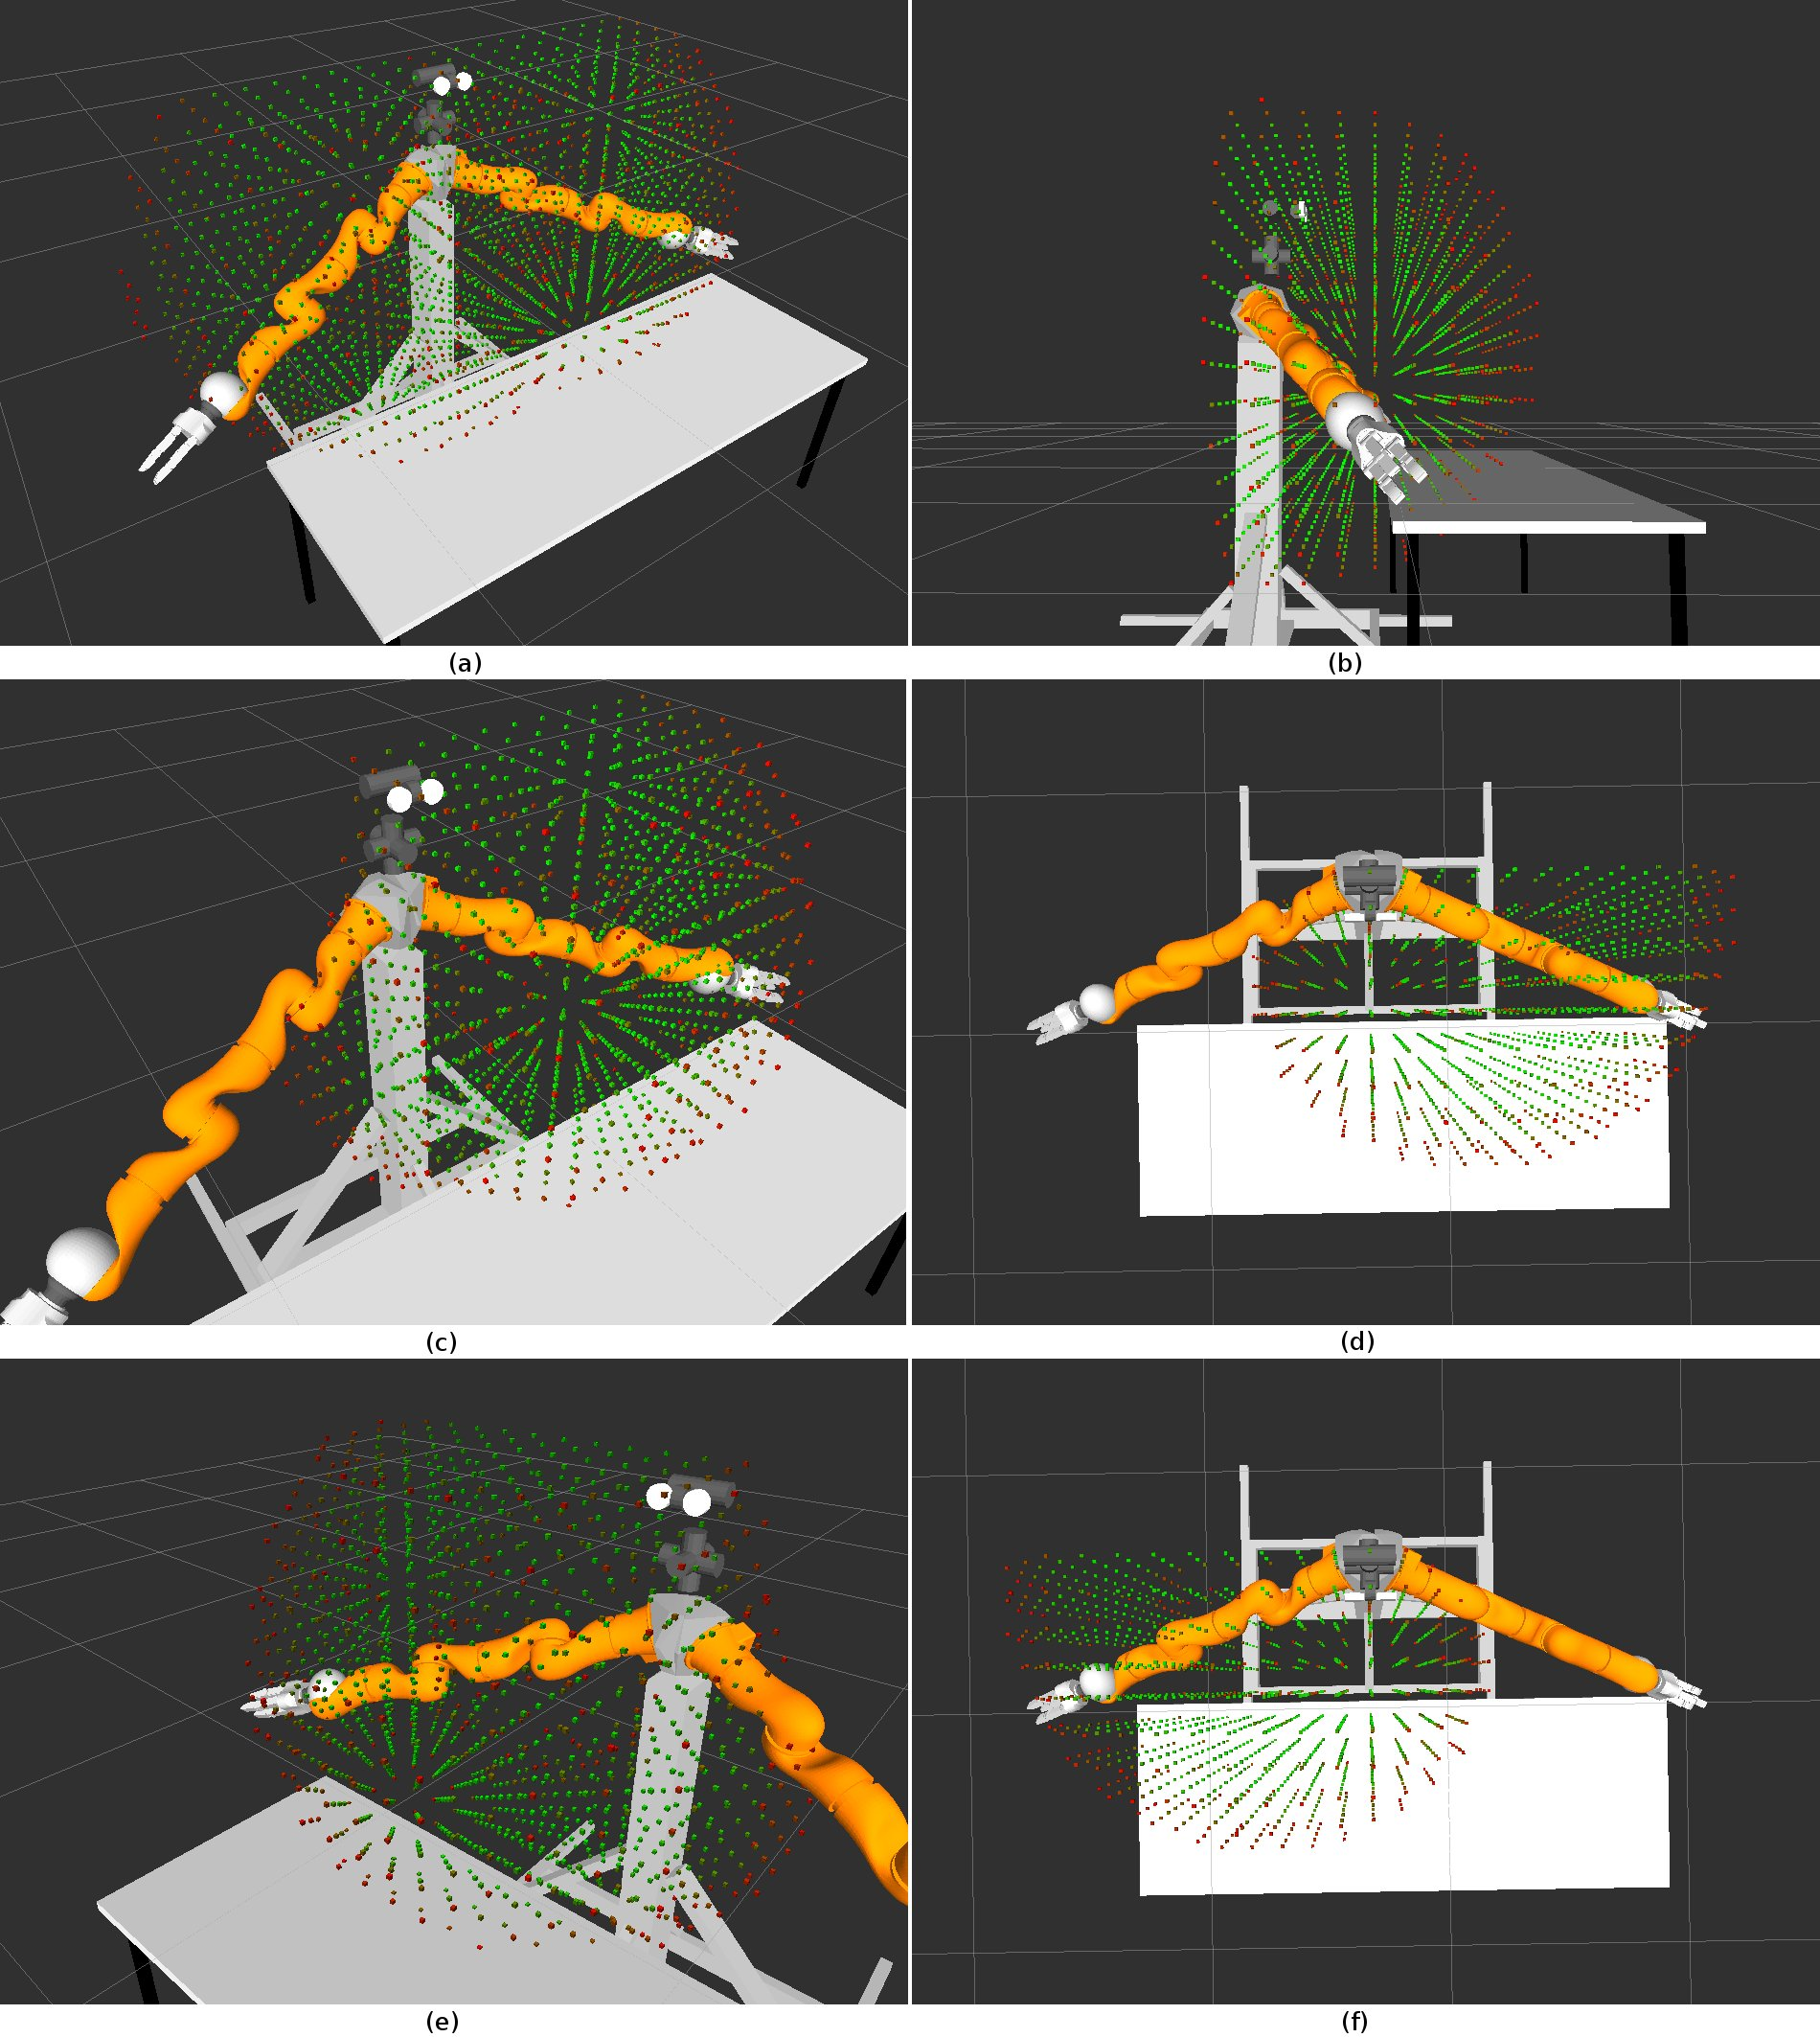
\includegraphics[width=1.0\textwidth]{images/results.jpg}
	\caption{IK test result visualization}
	\label{fig:ik_visualization}
\end{figure}


% Motion planning practical part
%!TEX root = thesis.tex

\chapter{Pick and place}
\label{chap:pick_place}

The implementation of a benchmark pick and place task which is executable on a simulator as well as on the real robot states one of the objectives of this project. The task consists of various stages which have to be planned using the planning framework introduced in the previous chapter. The overview at the beginning of this chapter provides information about general grasping tasks, explains the process step by step and describes the successive stages that have to be executed. The second part focuses on how pick and place tasks are planned and executed using the motion planning framework that was described in the previous chapter. The third section explains the implementation of the benchmark pick and place task in detail and describes the involved message types and action servers. The last section discusses some observations that have been made during the implementation process.

\section{Overview}

A pick and place task is the process of grasping an object, lifting it and dropping it at a target position. Humans can do that without even thinking about it. But directing a robot to perform a pick and place task reveals how difficult and complex it is and how much planning has to be involved to achieve the desired result. A planner would possibly require exact knowledge about the robot and it's environment, including the objects to grasp and the obstacles around. Collisions that could harm the robot have to be avoided but other collisions are necessary when the robot has to get in contact with the world. The gripper definitely collides with the object to pick, but only during grasping and holding. Therefore there has to be a mechanism to explicitly tell the planner that specific collisions are allowed during particular stages of the operation. Moreover, after grasping an object it has to be considered as an additional part of the robot. That means for the planning domain, that the grasped object should be included to the definition of the robot during subsequent planning requests because it possibly increases the size of the end effector that carries the object. \\

Stationary objects usually stand or lie on a surface, called the \emph{support surface}. During the interaction with an object, possible collisions with the support surface have to be taken into account. It is also possible that the whole process underlies additional constraints, so called \emph{path constraints}. This type of constraint has to be enforced along the whole path which the grasped object takes during the operation. For example, when carrying a glass filled with liquid it has to remain in an upright position, otherwise the liquid is lost. That means, the glass has to be held in a specific orientation during the whole task. This can be described as an so-called \emph{orientation constraint} which is a special type of a path constraint. The planning solution has to provide mechanisms to define and enforce such types of \emph{path constraints}. \\

\begin{figure}[ht]
	\centering
  	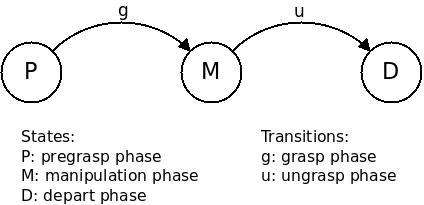
\includegraphics[width=0.5\textwidth]{images/state_trans.jpg}
	\caption{State transition diagramm for a pick and place task}
	{\scriptsize Image inspired by \citep{kang1994}}
	\label{fig:state_trans}
\end{figure}

\citep{kang1994} propose a method for \emph{temporal segmentation} of arbitrary grasping tasks. They divide each task into sequences of \emph{subtasks} that \emph{can be represented as series of states and transitions}. According to their notion, a pick and place operation is divided into 5 phases.

\begin{itemize}

\item \textbf{Pregrasp phase} \\

This phase starts at an arbitrary robot configuration. The hand is moved towards the grasp location and the fingers have to be adjusted to preshape the gripper in a way that allows to enclose the object to grasp (or at least that part that is used to clutch it). The required gripper configuration depends on the size and shape of the object to grasp and the structure of the gripper.

\item \textbf{Grasp phase} \\

This is the stage where the robot gets in contact with the object. The gripper closes around the object and applies as much force as necessary to be able to take and hold it. The grasp phase states the transition between the \emph{pregrasp} and the \emph{manipulation} phase.

\item \textbf{Manipulation phase} \\

The grasped object is enclosed by the gripper and considered to be part of the robot configuration. 
During \emph{manipulation} phase, the object is translated towards the place location. Possible path constraints have to be enforced whilst that stage.

\item \textbf{Ungrasp phase} \\

The manipulator reached at the goal location and the gripper opens and releases the object. This is the transition between \emph{manipulation} and \emph{depart} phase.

\item \textbf{Depart phase} \\

The object was placed at the target location and relased by the gripper. Now the manipulator retreats from the object. After that the entire task is completed.

\end{itemize}

The corresponding state transition diagram can be seen in Figure\ref{fig:state_trans}. The task is only considered to be complete if each single stage was successfully executed. Necessary planning parameters like the grasp location and gripper configurations are usually provided by a grasp planner. This is an additional node within the planning pipeline that can be used to identify objects in the environment of the robot, usually based on 3D sensor data and calculate the corresponding grasp parameters. Explaining the functionality of grasp planners is beyond the scope of this project though the section about implementing the reference task discusses the used parameters in greater detail and shows what data would usually be delivered by the grasp planner. \\

\section{Pick and place tasks in MoveIt}

\begin{figure}[ht]
	\centering
  	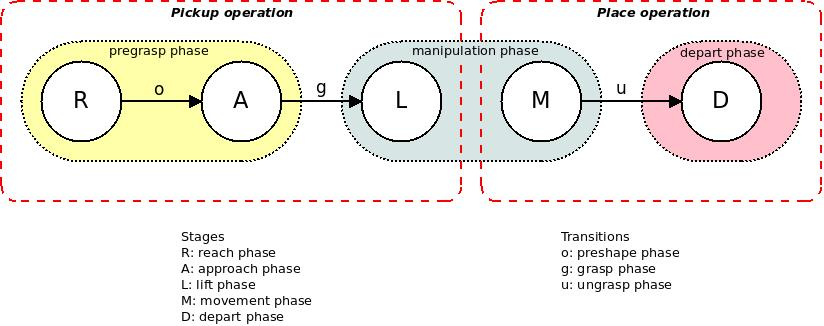
\includegraphics[width=1.0\textwidth]{images/pick_place_states.jpg}
	\caption{Extended state transition diagram}
	\label{fig:pick_place_states}
\end{figure}

The robot motions during the phases described in the previous section need to be planned. Each single stage requires to plan trajectories that are free of accidental collisions, respect the limits of the robot and enforce possible additional constraints. The task can only be considered executable if a valid motion plan for each single stage exists. Planning pick and place tasks in MoveIt requires to split them into two distinct operations, namely the \emph{pickup} operation and the \emph{place} operation. The explanation of those operations requires to further subdivide the phases described in the previous section. Figure \ref{fig:pick_place_states} shows the resulting state transition diagram.\\

The pickup operation starts at an arbitrary robot configuration. In the \emph{reach} stage, the manipulator has to be brought into a position close to the object to grasp, but in a distance which allows the gripper to open safely without touching the object. The \emph{preshape} stage sets the gripper into the \emph{pregrasp posture} which means the fingers are brought into a shape that allows to completely enclose the object (or at least that part that is used to clutch it). During the \emph{approach} phase the gripper moves towards the final grasp pose along the defined approach direction. The \emph{grasp} phase moves the gripper fingers into the \emph{grasp posture} - a configuration that encloses the object and applies as much force as necessary to be able to take and hold it. The resulting collisions between the gripper links and the object have to be ignored by the planner. From that point on the grasped object is \emph{attached} to the gripper, which means it is considered to be an additional part of the end effector during subsequent planning steps. The pickup operation completes lifting the object along the retreat direction (\emph{lift} phase). Figure \ref{fig:pickup} shows the stages of the pickup phase.

\begin{figure}[h]
	\centering
  	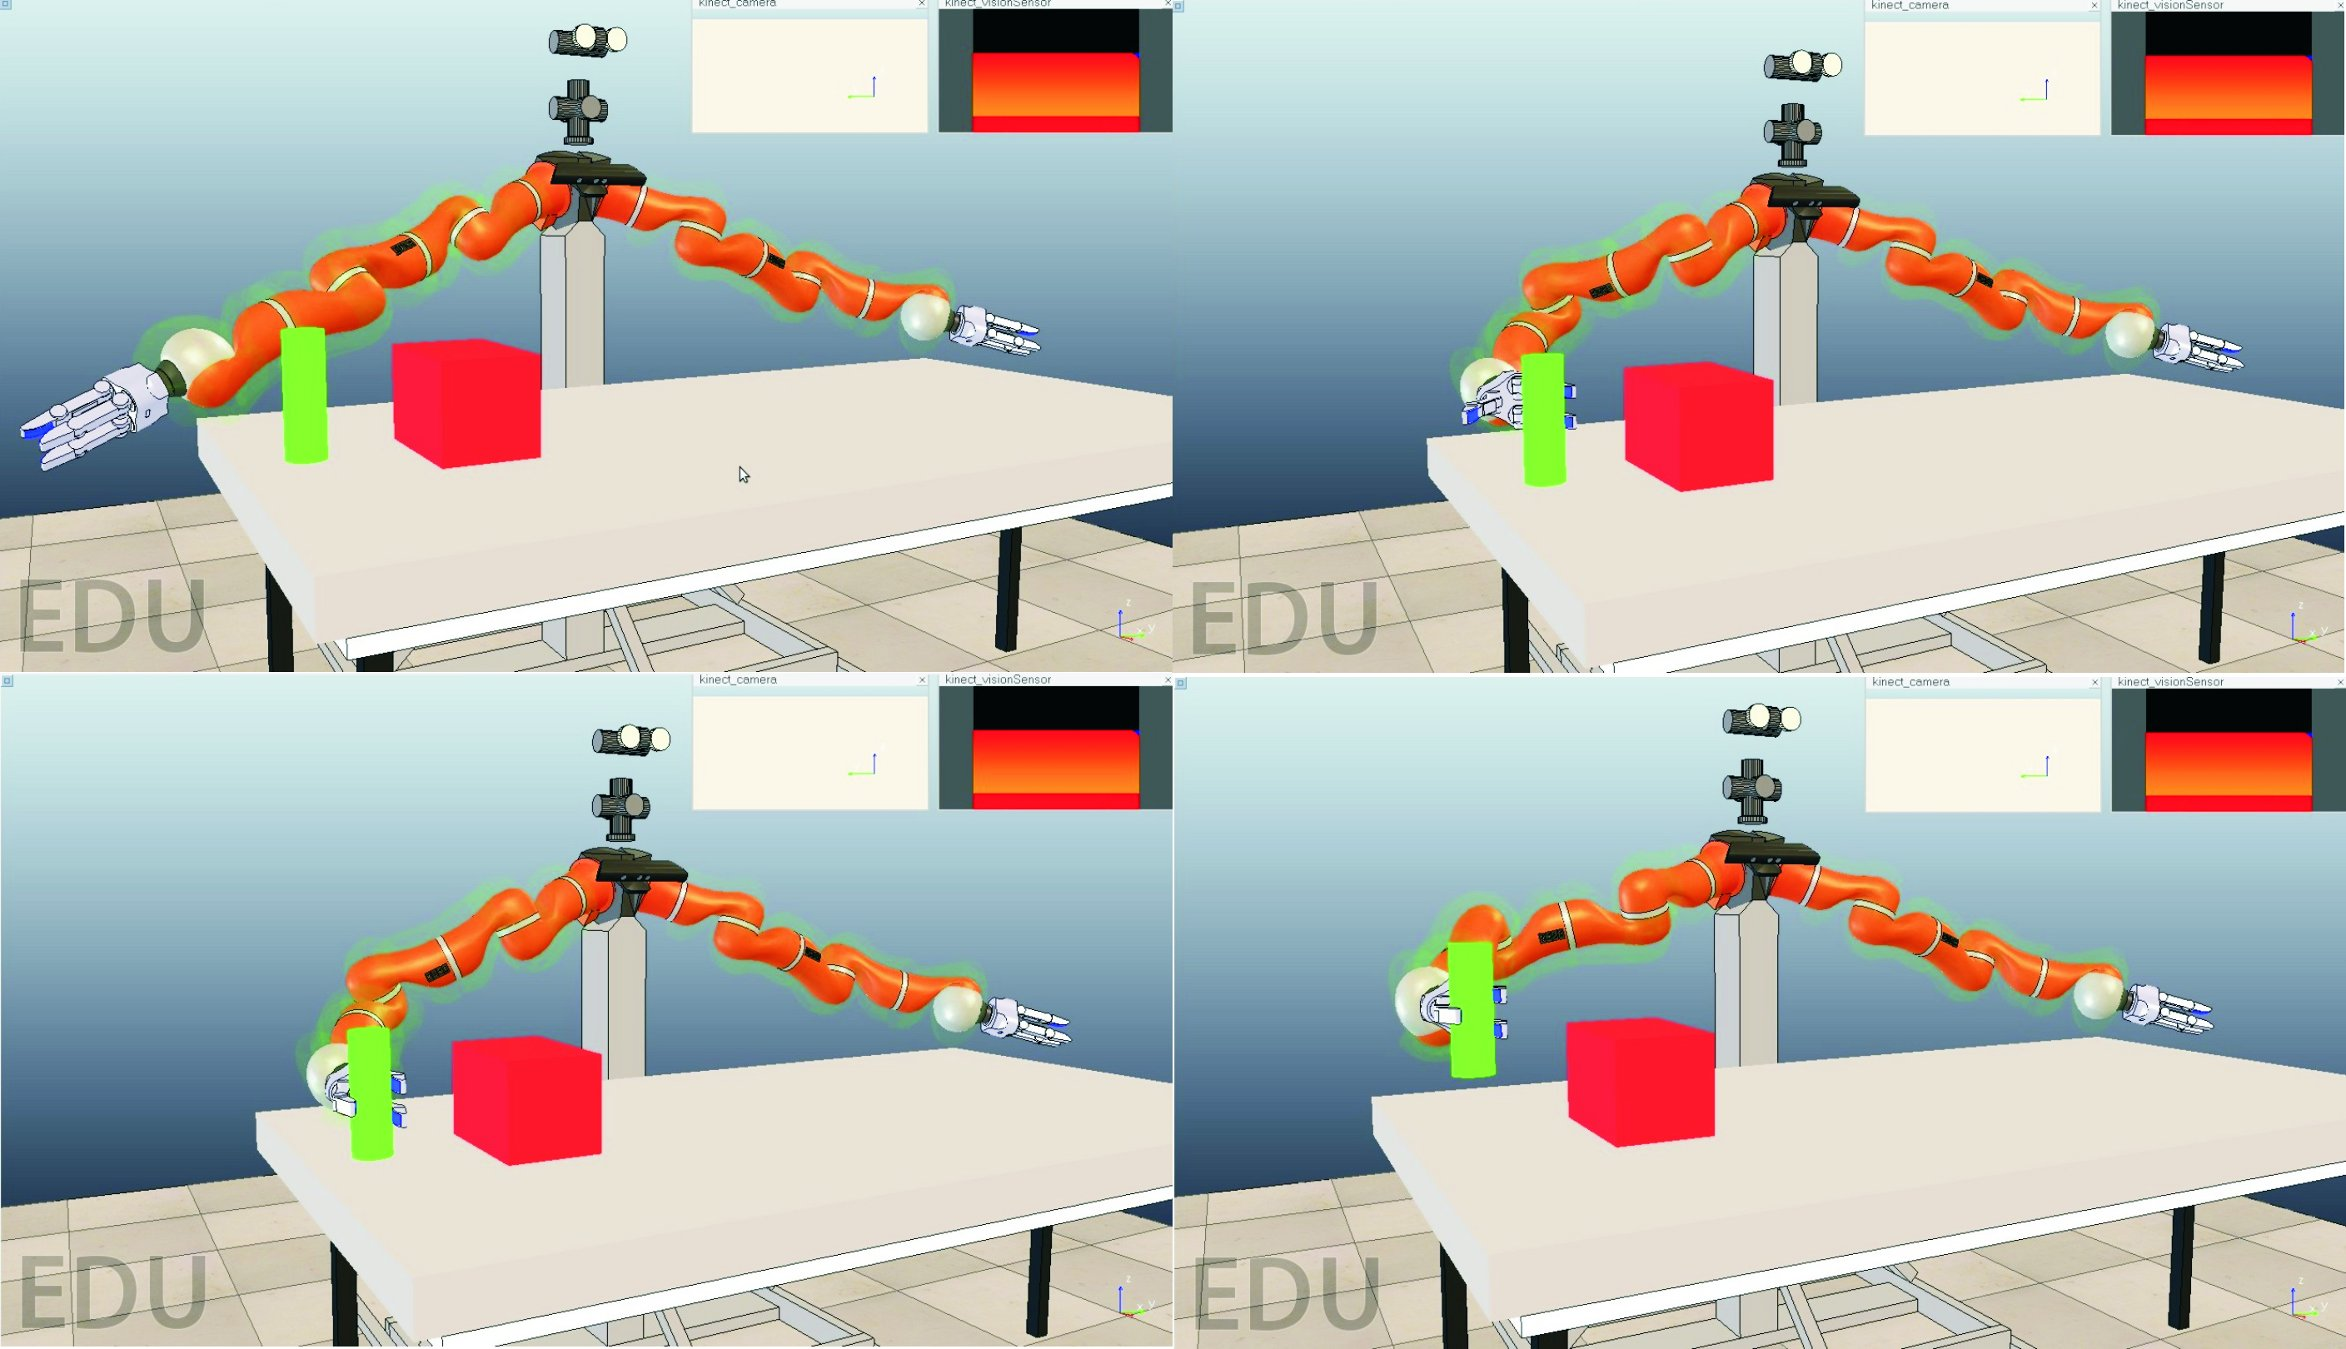
\includegraphics[width=0.75\textwidth]{images/pickup.jpg}
	\caption{Stages of the pickup phase in the simulator}
	\label{fig:pickup}
\end{figure}

The place operation starts after a successful pickup. The grasped object is enclosed by the gripper and it is considered to be part of the robot. During the \emph{movement} phase, the object is translated towards the final \emph{place location}. The planner has to take into account that the object could possibly get into contact with the support surface again when it's final position is reached. At that stage, the gripper opens (\emph{ungrasp} phase) and releases the object. Now the object has to be treated as an obstacle again and the planner is forced to avoid collisions with it. The place operation completes after the manipulator has moved away from the object (\emph{depart} phase) along the specified retreat direction. The stages of the placement phase can be seen in Figure \ref{fig:placement}.

\begin{figure}[h]
	\centering
  	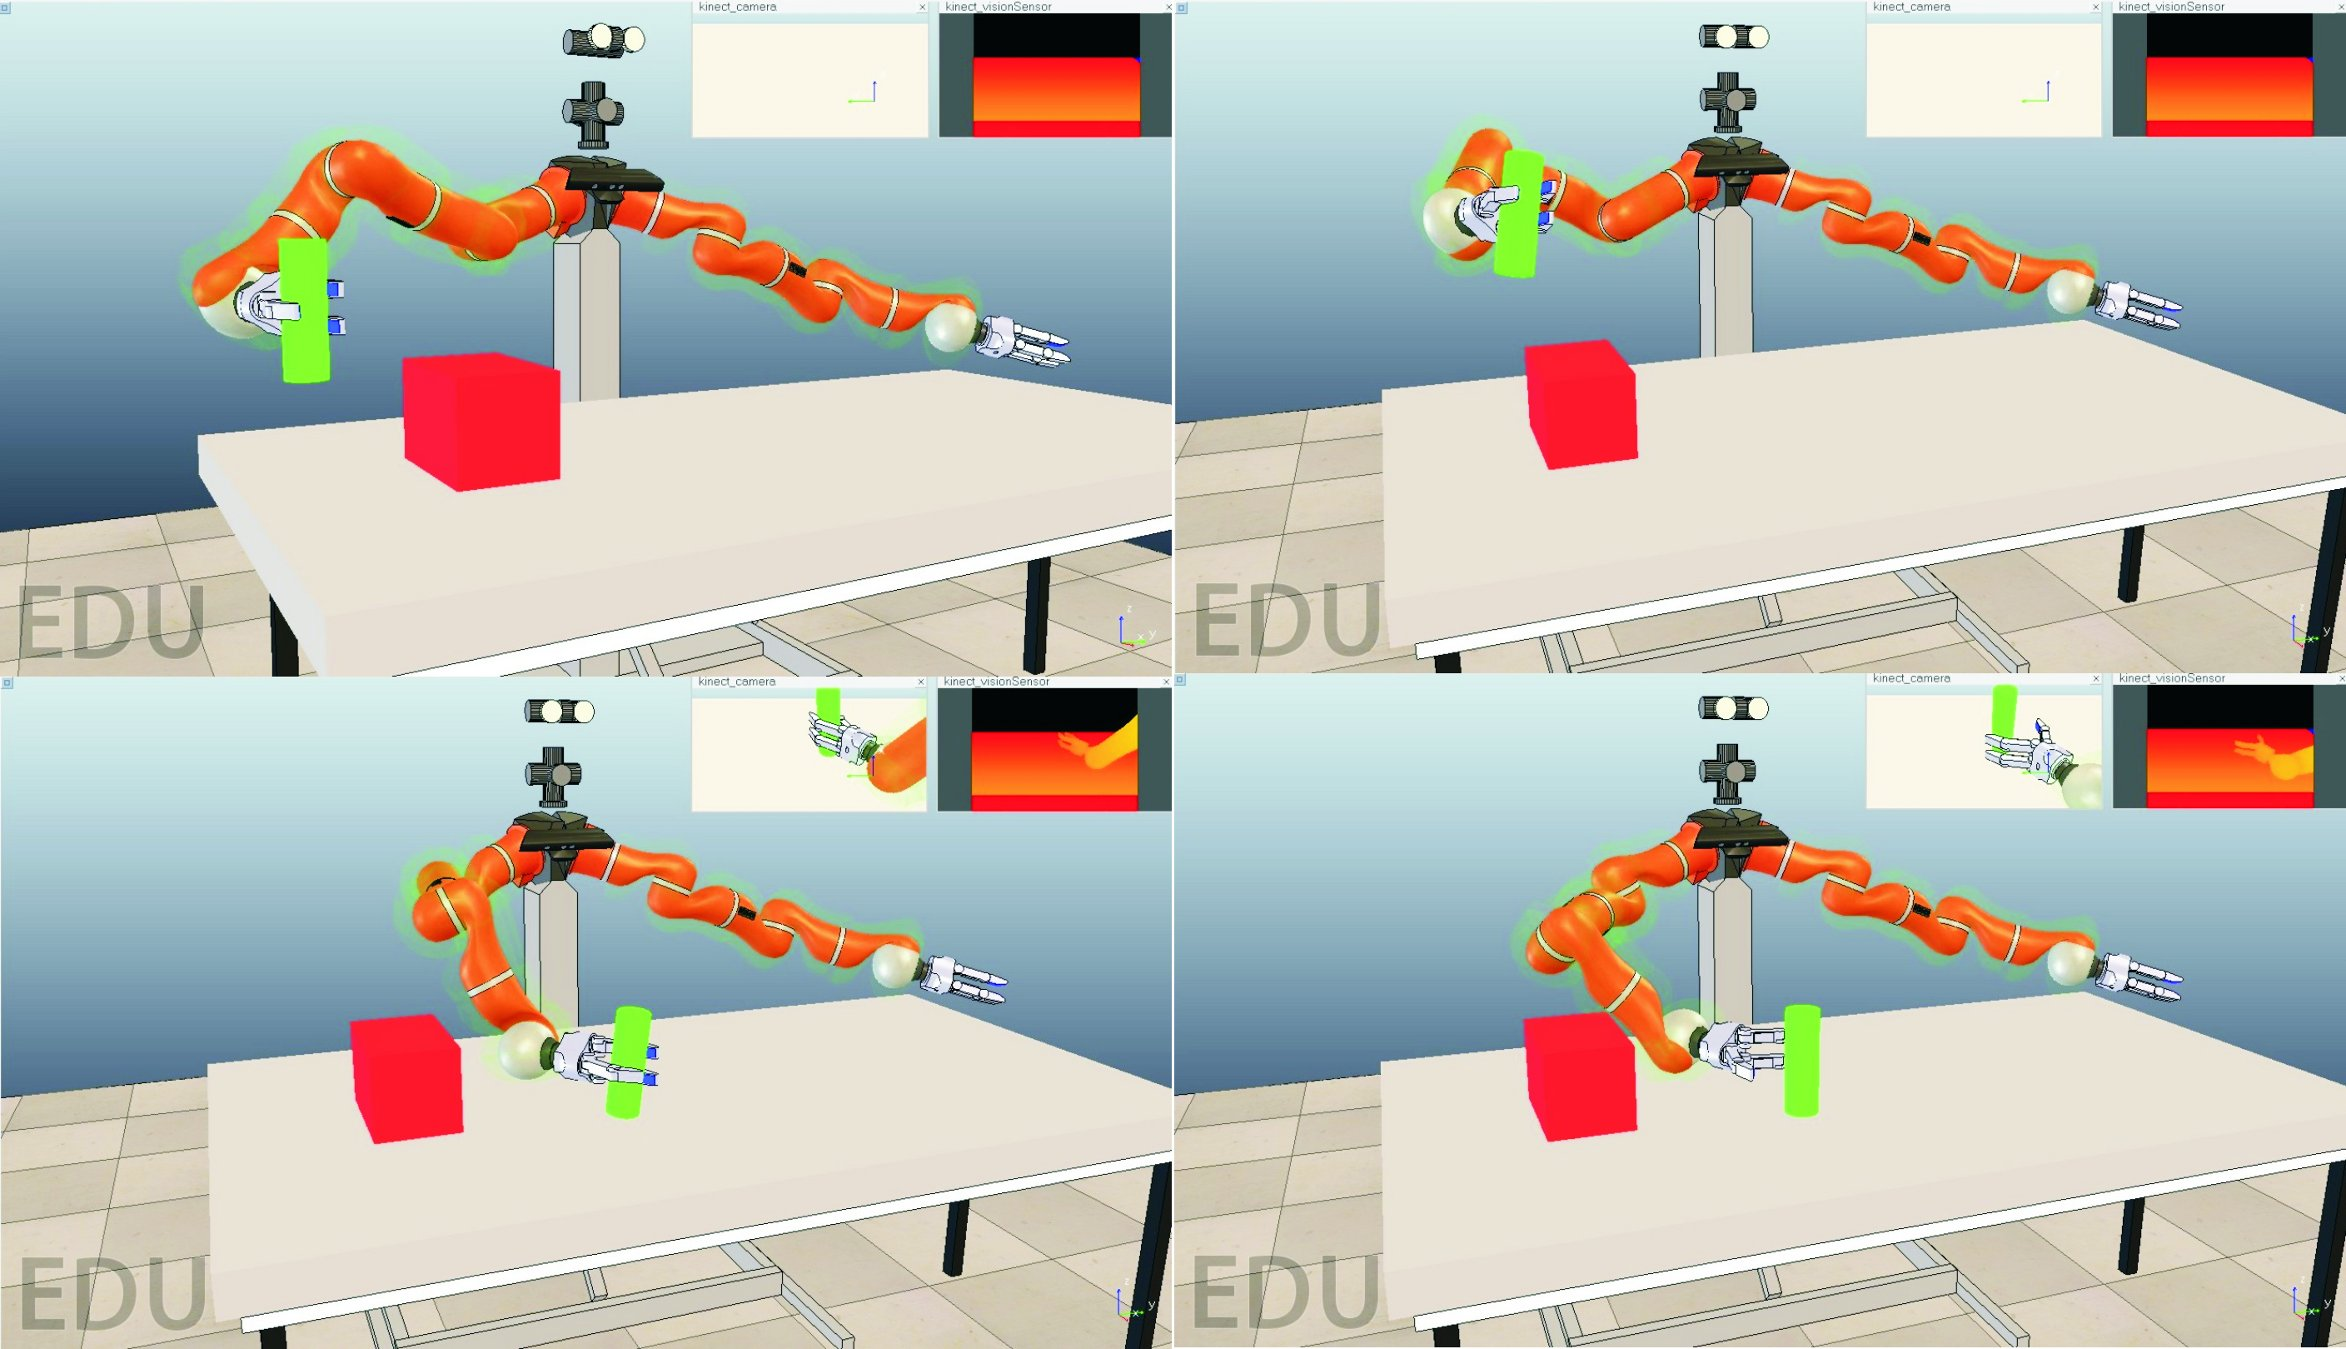
\includegraphics[width=0.75\textwidth]{images/placement.jpg}
	\caption{Stages of the placement phase in the simulator}
	\label{fig:placement}
\end{figure}

%The explanation of those operations requires to further subdivide the phases, described in the previous section. This results in the state transition diagram that can be seen in Figure \ref{fig:pick_place_states}. The pregrasp phase is split into \emph{reach}, hand \emph{preshape} and \emph{approach} phase. During the reach phase, the manipulator is moved into a position close to the object to grasp, but in a distance that allows the gripper to open safely without touching the object. This position is called the \emph{pre-grasp pose}. The approach phase brings the opened gripper towards the final \emph{grasp pose}. 
%The preshape phase is the transition between the reach and the approach phase. During that stage the gripper needs to  bring it's fingers into a configuration that allows to enclose the object. This configuration is called the \emph{pre-grasp posture}. The manipulation phase is divided into two phases, namely the lift phase and the movement phase. There is no transition between those two stages because the pickup operation completes after the lift phase and the place operation starts at the movement phase. Planning of those operations happens by using the corresponding action servers that are advertised by the \path{move_group} node.\\

%The structure of the request messages and the involved parameters are described in the next section. The result of a successful request is a motion plan that contains trajectories for all stages of the planned operation.

The planning of the described operations make use of action servers which are advertised by the \path{move_group} node, namely the \emph{pickup action server} and the \emph{place action server}. The pickup and placement requests are composed from a large number of parameters that are explained in detail in the next section. Objects contained in the task environment have to be added to the MoveIt planning scene. This can be done manually by publishing them to corresponding topics or by a MoveIt configuration to monitor the environment through sensor data, e.g. from a Kinect camera. For the sake of simplicity, all involved objects were manually added in the benchmark task. Pickup- and place action servers provide the ability to choose whether to execute motion plans immediately or to just perform the planning part and return the resulting trajectories for later execution. Immediate execution is often preferable because MoveIt executes the trajectories and handles additional requirements like attaching and detaching the grasped object in time. It has the drawback, however, that occasionally overly long and unnatural trajectories are executed immediately because they might be formally valid solutions for the given planning problem, though they are unsuitable for a human observer. Therefore a safety mechanism which can interrupt an execution in face of problems needs to be added. The second, planning-only method allows to visualize the resulting trajectories and then decide whether to execute them or not. But then each single trajectory stage has to be executed manually which also includes attaching or detaching objects to the manipulator. The advantage of this method is the clean separation between planning and execution, allowing maximum control over the execution flow. Therefore this method was favoured during benchmark task implementation.

\section{Implementation of the benchmark task}

This section describes the implementation of the benchmark pick and place task in detail. The source code can be found in the \path{uibk_moveit_tests} package. The workspace is the table in front of the robot covered with a 9 cm thick foam mat. This mat will be declared as the support surface later on. The object to grasp is a cylinder with 4 cm radius and a height of 25 cm. The cylinder is located on a fixed, known position. A cube with an edge length of 20 cm acts as additional obstacle within the workspace. The goal of the task is to pick the cylinder up, using the right arm of the robot and place it at the goal location without colliding with the obstacle or other parts within the robot's environment. The implementation makes use of the previously described pick and place functionality. The necessary steps are explained in the following subsections.

\subsection{Creating the environment}
\begin{figure}[h]
	\centering
  	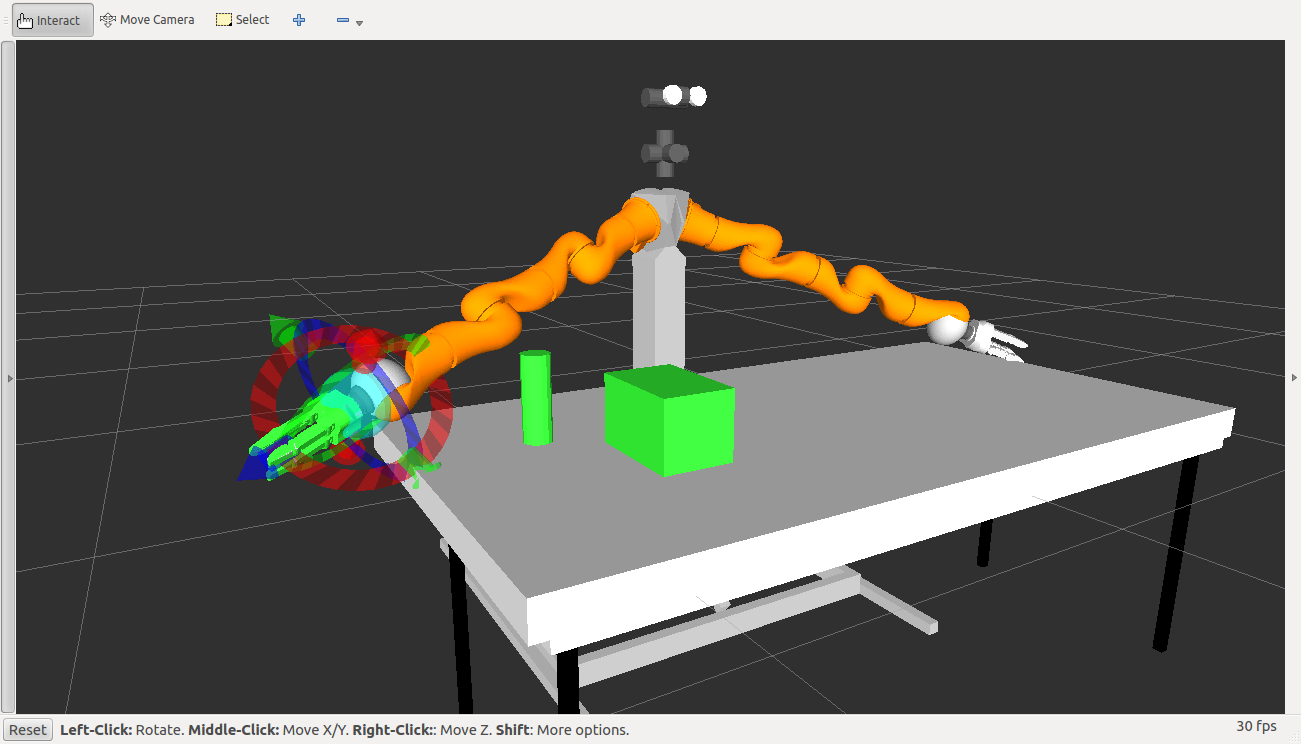
\includegraphics[width=0.75\textwidth]{images/task_env.png}
	\caption{Planning scene after inserting the collision objects}
	\label{fig:task_env}
\end{figure}
As MoveIt is currently not configured to use sensor data, it has to be informed about the task environment. The table and the surface mat (\path{table_surface_link}) are already part of the URDF description but the cylinder and the obstacle have to be added to the planning scene. This is done utilizing the \emph{PlanningSceneInterface} class that provides functionality to manipulate the current planning scene. The \emph{CollisionObject} type is used to describe those objects. Both of them are primitive shapes. Necessary parameters are the shape type, dimensions and pose. Additionally each \emph{CollisionObject} needs a unique ID which is used to identify the shape within the planning scene. Listing \ref{lst:obstacle} shows the necessary code for creating the obstacle, Figure \ref{fig:task_env} shows a visualization of the task environment after adding the \emph{CollisionObjects}.

\lstset{style=customc}
\begin{minipage}{\linewidth}
\begin{lstlisting}[caption={Creating the obstacle}, label=lst:obstacle]
std::vector<moveit_msgs::CollisionObject> collision_objects;
// create an obstacle
shape_msgs::SolidPrimitive box;
box.type = box.BOX;
box.dimensions.resize(3);
box.dimensions[0] = 0.2;
box.dimensions[1] = 0.2;
box.dimensions[2] = 0.2;

/* A pose for the box (specified relative to frame_id) */
geometry_msgs::Pose box_pose;
box_pose.orientation.w = 1.0;
box_pose.position.x = 0.15;
box_pose.position.y = 0.10;
box_pose.position.z = 0.1 + SUPPORT_SURFACE_HEIGHT;

obstacle.primitives.push_back(box);
obstacle.primitive_poses.push_back(box_pose);
obstacle.operation = obstacle.ADD;

collision_objects.push_back(obstacle);
// Now, let's add the collision object into the world
planning_scene_interface_->addCollisionObjects(collision_objects);
\end{lstlisting}
\end{minipage}

\subsection{Generating possible grasps}

\begin{figure}[h]
	\centering
  	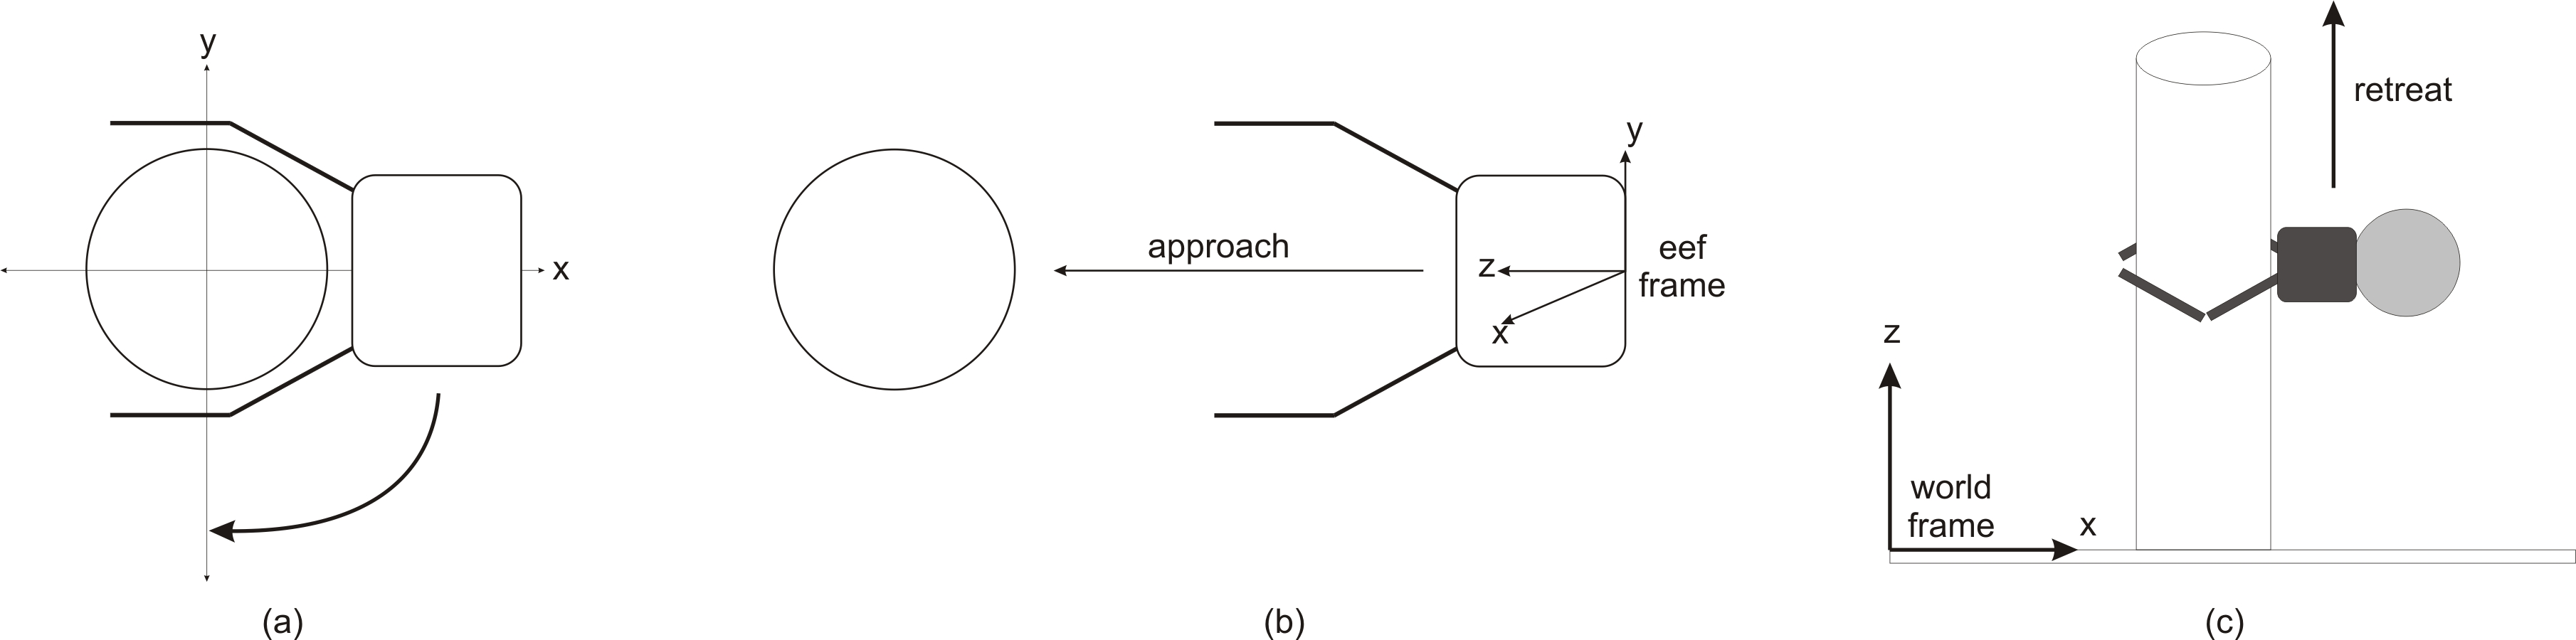
\includegraphics[width=1.0\textwidth]{images/grasp_a-c.jpg}
	\caption{Grasp poses, gripper approach and retreat}
	\label{fig:grasp_stages}
\end{figure}

Picking up an object can always be done in several ways. Depending on the shape of the object there always multiple alternatives how gripper can safely approach and grasp. Providing a number of different grasps raises the probability that the pickup request will be successful. Before calling the pickup action server it is necessary to generate a set of possible grasps for the object to pick. This information is usually provided by a grasp planner. The sample task encapsulates the grasp planner functionality within the \path{generateGrasps()} method. This method takes the current pose of the cylinder as input and calculates 10 possible grasp poses along an imaginary circle segment around the cylinder location (Figure \ref{fig:grasp_stages}a). Grasps are defined in terms of the \emph{Grasp} data structure. The following paragraphs describe the involved parameters and how they were determined in the benchmark task implementation.

\paragraph{Grasp ID} A string that uniquely identifies the grasp. As usually many different grasps are provided for each pickup request, this ID can be used to identify the grasp which is finally picked to solve the planning problem. The grasp IDs are formed according to the pattern \texttt{[Grasp]x}, where $x \in [0,10]$ 

\paragraph{Pre-grasp/grasp posture} Describes the shape of the hand before/after grasping the object.
Pre-grasp and grasp postures are joint trajectories for the gripper, containing just one trajectory point stating the target configuration for the gripper in the opened respectively the closed state.

\paragraph{Pre-grasp approach and post-grasp retreat} The pre-grasp approach and the post-grasp retreat are defined as \emph{GripperTranslation}, as can be seen in Listing \ref{lst:translation}. This is a special message type that describes the direct gripper movement from one position towards a target. The direction is defined as a three dimensional vector. The length of the translation can be set in a flexible way by specifying a desired distance and a minimum distance. That means that the location where the gripper needs to open is not explicitly set and can be any point along the approach vector between minimum distance and desired distance. Experiments showed that the success rate is higher if the grasp parameters allow some flexibility to the planner at certain points. The approach vector depends on the grasp pose and points along the z-axis of the end effector frame towards the object (Figure \ref{fig:grasp_stages}b). The gripper retreat vector points up, along the z-axis of the world (Figure \ref{fig:grasp_stages}c).

\lstset{style=customc}
\begin{minipage}{\linewidth}
\begin{lstlisting}[caption={Definition of gripper translations}, label=lst:translation]
// gripper approach
GripperTranslation gripper_approach;
gripper_approach.desired_distance = 0.2; // cm
gripper_approach.min_distance = 0.1; // cm
gripper_approach.direction.header.frame_id = EE_PARENT_LINK;
gripper_approach.direction.vector.x = 0;
gripper_approach.direction.vector.y = 0;
gripper_approach.direction.vector.z = 1;
new_grasp.pre_grasp_approach = gripper_approach;

// gripper retreat
GripperTranslation gripper_retreat;
gripper_retreat.desired_distance = 0.2; // cm
gripper_retreat.min_distance = 0.1; // cm
gripper_retreat.direction.header.frame_id = BASE_LINK;
gripper_retreat.direction.vector.x = 0;
gripper_retreat.direction.vector.y = 0;
gripper_retreat.direction.vector.z = 1;
new_grasp.post_grasp_retreat = gripper_retreat;
\end{lstlisting}
\end{minipage}

\paragraph{Grasp pose} The grasp pose specifies the position and orientation of the end effector during the grasp stage as can be seen in Figure \ref{fig:grasp_pose}. The function in \ref{eq:grasp_pose} is used to calculate the grasp pose based on angle $\theta$. 
\begin{equation} \label{eq:grasp_pose}
f(\theta) = 
\begin{pmatrix}
x_{\theta} \\
y_{\theta} \\
z_{\theta} \\ 
roll_{\theta} \\
pitch_{\theta} \\
yaw_{\theta}
\end{pmatrix} =
\begin{pmatrix}
-r\sin(\theta) \\
r\cos(\theta) \\
0 \\ 
\frac{\pi}{2} \\
\theta \\
-\frac{\pi}{2}
\end{pmatrix}
\end{equation}
Parameter $r=19cm$ specifies the distance between the eef link and the object center. Grasp poses are calculated for 10 different angles $\theta$ from the interval $[\pi, \frac{\pi}{2}]$. All poses are computed relative to the cylinder reference frame and then converted to the reference frame of the world.

\begin{figure}[ht]
	\centering
  	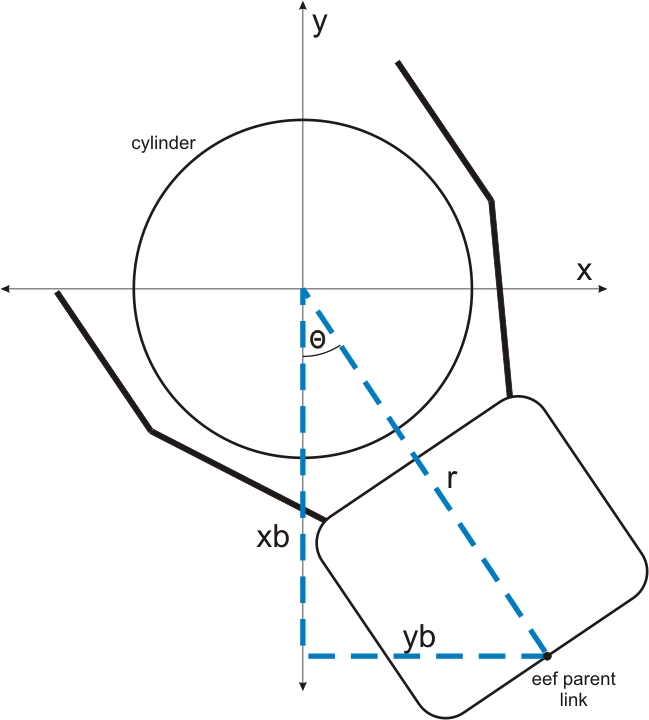
\includegraphics[width=0.4\textwidth]{images/grasps.jpg}
	\caption{Grasp pose determination}
	\label{fig:grasp_pose}
\end{figure}

\paragraph{Grasp quality} This parameter allows to tell the planner, how `good' a specific grasp is, i.e. how likely it is that the grasp can be successfully executed. MoveIt can then favour grasps with higher quality if several valid solutions are found by the planner. As none of the generated grasps should be favoured among the others, all grasps use the quality parameter value $1.0$, which indicates that they are equal in quality.

\paragraph{Allowed touch objects} A list, containing the identifiers of the objects, that are allowed to be touched when using that specific grasp. In the benchmark task, this is only the grasped object.

\subsection{Planning and executing the pickup}

After generating the set of grasps, the pickup operation can be planned. The \emph{PickupAction} server handles planning and optionally the execution of all stages of a pickup operation at once. The request is done, using a \emph{PickupAction} client to send \emph{PickupGoal} messages to the server. The required parameters of the request message are described in the subsequent paragraphs.

\paragraph{\texttt{target\_name}} The name of the object to pick which is the ID that was used when adding the object to the planning scene.
\paragraph{\texttt{group\_name}} The name that identifies the planning group that should be used to perform the pickup, i.e. \path{right_arm}.
\paragraph{\texttt{end\_effector\_name}} The name of an end effector in the specified planning group. This is necessary because it is possible to define planning groups that contain multiple end effectors.
\paragraph{\texttt{possible\_grasps}} The set, containing the previously computed grasps. At least one grasp has to be provided, but the success rate rises when providing multiple grasps.
\paragraph{\texttt{support\_surface\_name}} The name of the link that acts a support surface within the planning scene. This is the link that states the surface mat covering the table (\path{table_surface_link}). 
\paragraph{\texttt{allow\_gripper\_support\_collision}} That parameter specifies, whether collisions between the gripper links and the support surface are allowed, or not.
\paragraph{\texttt{path\_constraints}} It is possible to apply a set of path constraints to the planning request. This could be for example an orientation constraint for the end effector. Path constraints are enforced on each single point of the resulting trajectory which drastically raises the complexity of the planning problem. The sample task does not apply any task constraints.
\paragraph{\texttt{allowed\_planning\_time}} The maximum amount of time, the planner is allowed to find a solution. The sample tasks uses a value of 5 seconds.
\paragraph{\texttt{plan\_only}} Specifies, if resulting trajectories should be immediately executed, or not. This is set to \path{true} to allow a visual validation of the resulting motion plan. \\

On success, the pickup action server returns a motion plan, containing trajectories for all stages of the pickup operation. MoveIt automatically publishes planned trajectories to the \path{move_group/display_planned_path} topic. RViz can be configured to display the trajectories published to that topic. If a visual validation results in a satisfying solution it can be executed on the \path{execute_kinematic_path} service, which is advertised by the \path{move_group} node. The service sends given trajectories to the responsible controller and provides feedback information about the execution status in the service response message. The pickup phase completes after successful execution of all trajectory stages.

%A reusable helper class was created that can be used to simplify all kinds of planning requests. The utility class is called \emph{PlanningHelper} and can be found within the \path{uibk_planning_node} package. A call to the pickup action server is done by using the \path{plan_pick()} method of the helper class. This method takes the a set of possible grasps and the ID of the object to pick as parameters. The outcome is a pointer to an instance of \emph{PlanningResult}, a structure that contains all the necessary information about a planning attempt. Success or failure is indicated by the \path{status} parameter. On success, the parameter \path{trajectory_stages} holds a vector, containing the resulting trajectory stages. The actual planning request is done, using a \emph{PickupAction} client to send \emph{PickupGoal} messages to the pickup server. The message is composed from  the ID of the object to pick, the previously computed grasps, the name of the chosen planning group and the name of the link within the robot model that acts as the support surface. Optional parameters are among others the ID of the planner to use and the maximum allowed planning time. The parameter `plan\_only' within the planning options is set to true to avoid the immediate execution of the planned trajectories. This allows a visual verification of the planning outcome before execution. The resulting robot path is shown in RViz. If the solution is satisfying it can be executed, passing the PlanningResult to the corresponding method of the PlanningHelper class. This method uses the `/execute\_kinematic\_path' service provided by the `move\_group' node. The service sends a given trajectory to the responsible controller and provides feedback information about the execution status. The `PlanningHelper' also takes care to attach the picked object to the gripper after the grasp stage. The pickup phase completes after successful execution of all trajectory stages.


\subsection{Planning and executing the placement}

The placement phase is planned and executed in a similar manner. The cylinder has to be placed on a specific location within the workspace in an upright position - the rotation around the z-axis doesn't matter. Therefore a set of possible place poses is generated in 20 different orientations around the z-axis (Figure \ref{fig:place_stages}a), allowing the planner to choose which one to use. The final approach towards the goal location is specified as \emph{GripperTranslation}. The direction vector points down along the z-axis of the world (Figure \ref{fig:place_stages}b). Desired and minimum distances are set to 20 cm and 10 cm respectively. The same pre-grasp posture configuration is used for the post-place posture. The last required parameter for a place location is the \emph{GripperTranslation} which describes the retreat after releasing the object at the target location. The direction depends on the chosen orientation and points towards the negative z-axis of the gripper reference frame (Figure \ref{fig:place_stages}c). 

\begin{figure}[ht]
	\centering
  	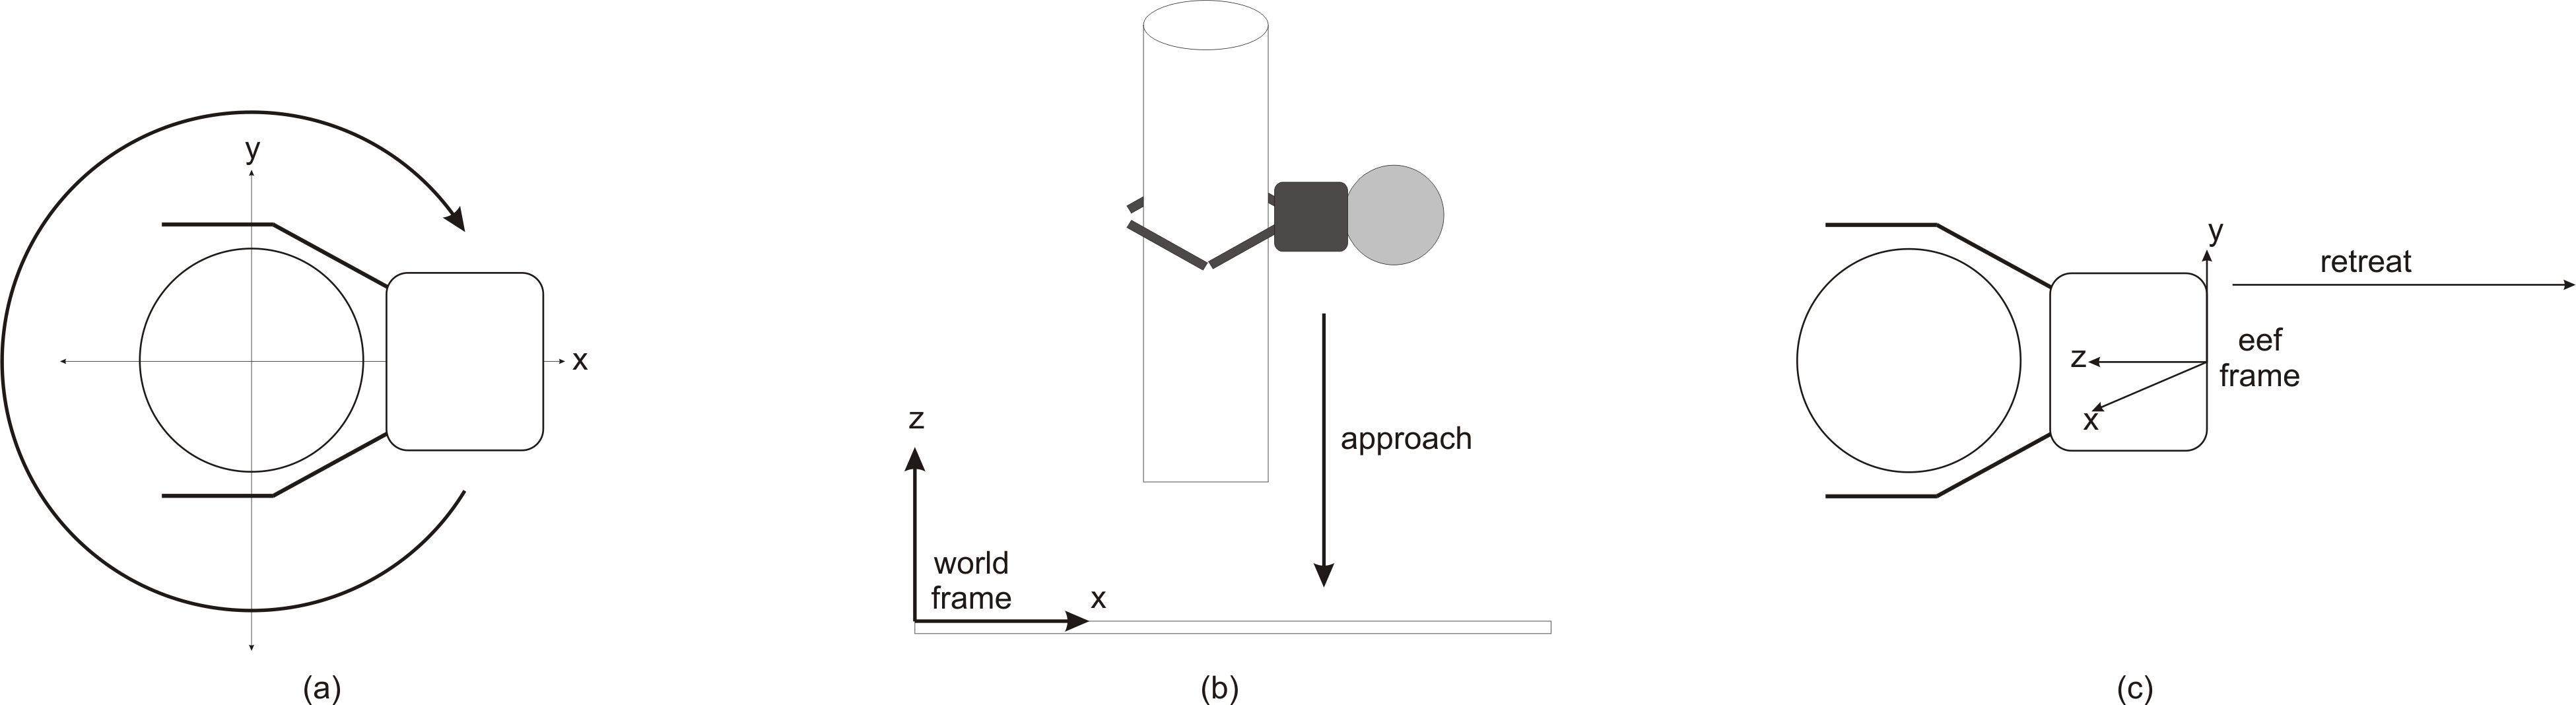
\includegraphics[width=1.0\textwidth]{images/place_a-c.jpg}
	\caption{Place locations, pre-place approach and post-place retreat}
	\label{fig:place_stages}
\end{figure}

The \emph{PlaceAction} server is responsible for planning the whole placement phase. The request utilizes a \emph{PlaceAction} client and \emph{PlaceGoal} messages. The server call is done in the same way as in the pickup phase. The most important parameters are the ID of the object to place, the name of the planning group, the set of possible place locations and the maximum allowed planning time.  On success, again the resulting trajectories are visualized in RViz and can be executed after positive validation. After execution, the task is considered to be completed and the picked object is detached from the gripper and again part of the collision world.


\section{Running the benchmark task}

The benchmark task is designed to run on the simulator and with the real robot as well. It only depends on a running \path{move_group} instance. Therefore it is necessary to start the simulator or real robot and launch the corresponding MoveIt instance as described in Section \ref{sec:launch_moveit}. The benchmark task can then be executed in the desired namespace. This is done by setting the \path{ROS_NAMESPACE} environment variable to either \path{simulation} or \path{real} within the terminal that is used to run the task. The following example runs the benchmark task on the simulator.

\begin{quote}
\begin{verbatim}
export ROS_NAMESPACE=simulation
rosrun uibk_moveit_tests sample_pick_place 
\end{verbatim}
\end{quote}

After creating the environment and adding the objects to the planning scene the pickup phase gets planned. The outcome can be seen in RViz and the program will ask if the resulting trajectory is ok and should be executed. A negative answer will force the program to replan the pickup and ask again, otherwise the trajectory gets executed. After successful execution, the place phase gets planned. The resulting plan is visualized as well and its execution also needs confirmation. The program exits after successful completing the placement phase. Listing \ref{lst:pick_place} shows the main routine of the benchmark task. It was observed that planning sometimes fails due to unknown MoveIt internal issues and subsequent calls with the same parameters are successful. Therefore, the pickup and the place operation are handled within a loop. 

\lstset{style=customc}
\begin{minipage}{\linewidth}
\begin{lstlisting}[caption={Benchmark task main routine}, label=lst:pick_place]
bool start() {
	// create obstacle and object to move...
	createEnvironment();

	bool picked = false;
	while (!picked && ros::ok()) {
		if (!pick(start_pose_, OBJ_ID)) {
			ROS_ERROR_STREAM_NAMED("pick_place", "Pick failed. Retrying.");
			// ensure that object is detached from gripper
			cleanupACO(OBJ_ID);
		} else {
			ROS_INFO_STREAM_NAMED("pick_place",	"Done with pick!");
            picked = true;
		}
	}

	ROS_INFO_STREAM_NAMED("simple_pick_place", "Waiting to put...");
	ros::Duration(5.5).sleep();

	bool placed = false;
	while (!placed && ros::ok()) {
		if (!place(goal_pose_, OBJ_ID)) {
			ROS_ERROR_STREAM_NAMED("pick_place", "Place failed.");
		} else {
			ROS_INFO_STREAM_NAMED("pick_place", "Done with place");
			placed = true;
		}
	}
	return true;
}
\end{lstlisting}
\end{minipage}

\section{Discussion}

This section gives an overview of the most important observations that have been made during the implementation of the sample task:

\begin{itemize}

\item

It is very important to provide some degree of freedom to the planner at various points. This is achieved by providing various grasps and place locations during planning requests. The definitions of gripper translations like pre-grasp approach, post-grasp retreat, pre-place approach and post-place retreat also allow to add additional flexibility by setting the desired and minimum distance values accordingly. Very strictly defined planning requests are very likely to fail whereas requests with a higher degree of flexibility drastically raise the overall success rate.

\item

Working with path constraints drastically drops the success rate because of the high complexity of the planning problem. Enforcing path constraints results in a drastically increased planning time and a large number of necessary IK requests. Therefore no path constraints were used within the sample task. It is possible, that a faster IK solution than the one that is currently utilized could help to solve the problem but that was not tested in this project.

\item

It was observed that sometimes planning requests seem to fail due to some MoveIt-internal issues and not because planning was not possible at all. Therefore it is necessary to repeat failed requests because it is very likely that planning succeeds on subsequent attempts. In the sample task implementation, the planning requests are done within a loop. If a request fails, it gets repeated a couple of times. A successful request breaks the loop and continues the execution flow. This strategy is obviously only feasible in the reference task because its configuration was designed to be plannable and executable.

\item

Resulting trajectories should always be visualized and validated before confirming the execution. This can be done, using RViz and/or the simulator. The calculated motion plans might be valid in terms of the defined goal constraints but sometimes they are overly long and unnatural and therefore unsuitable. Moreover, the planner can only take into account what it knows about the robot's environment. Especially in the robot lab the environment changes frequently when new equipment is mounted in the area around the robot. Therefore the visual validation is particularly important to avoid damages on the robot and its environment.

\end{itemize}



% Conclusion, possible further work, open questions
%!TEX root = thesis.tex

\chapter{Conclusions}
Current status, open questions, possible further work

\bibliography{refs}% Remember to compile the bibliography using bibtex.

\appendix% Start your appendices with this command.
% Implementation details, documentations...
%!TEX root = thesis.tex

\chapter{Simulator Plugin documentation}

%!TEX root = thesis.tex

\chapter{URDF descriptions}
\label{app:urdf}

\lstset{style=customxml}

\section{Complete model with table}
\lstinputlisting[caption={iis\_robot\_table.xacro}, label=lst:urdf_robot_table]{code/iis_robot_table.xacro}

\section{Adjusted gripper model}
\lstinputlisting[caption={sdh\_with\_connector.xacro}, label=lst:urdf_sdh]{code/sdh_with_connector.xacro}

\section{Torso model}
\lstinputlisting[caption={torso.xacro}, label=lst:urdf_torso]{code/torso.xacro}

\section{Table model}
\lstinputlisting[caption={table.xacro}, label=lst:urdf_table]{code/table.xacro}

\end{document}
